\chapter{Overview of One Dimensional Results}

	In this chapter we will give an overview of results pertaining to the one-dimensional family $f_{c, \beta} (x) = x^2 + c + \frac{\beta}{x^2}$ where $x, c, \beta \in \R$. Furthermore, we will fix the parameter $\beta$ at $.001$ and consider the structure of the resulting system $f_{c} (x) = x^2 + c + \frac{.001}{x^2}$ as the parameter $c$ is varied. Comparisons will be drawn against the standard quadratic map $Q_c (x) = x^2+c$ and the results which are proven in the next chapter will be introduced and discussed.


	\section{Preliminary Numerical Experiments}\label{res:prelim}

		When first considering some dynamical system, the critical points tend to be a focus of preliminary attention because they play an important role in the overall dynamics of the system. To see why, we introduce the Schwarzian Derivative and a theorem which tells us how the critical orbit can help determine the behavior of all other orbits.

		\begin{mydef}{Schwarzian Derivative\cite{Dev1} }
		The Schwarzian Derivative of a function $F$ is given by:
		\[
			SF (x) = \frac{F''' (x)}{F' (x)} - \frac{3}{2} \left (\frac{F'' (x)}{F' (x)}\right)^2
		\]
		\end{mydef}
		\begin{myth}\label{sch}
			Suppose $SF (x) < 0 \ \forall x$ where $SF$ is the Schwarzian Derivative of some function $F$. Then, if $x_0$ is an attracting periodic point for $F$, either the immediate basin of attraction of $x_0$ extends to $+\infty$ or $-\infty$, or else there is a critical point of $F$ whose orbit is attracted to the orbit of $x_0$\cite{Dev1}.
		\end{myth}

		
		For our family, as a rational map of $\R$, infinity is attracting so no attracting periodic orbit can have a basin of attraction which extends to $\pm\infty$. Thus if an attracting periodic orbit exists in a system such as ours, which also has a negative Schwarzian Derivative, then the orbit of the some critical point will be attracted towards that periodic orbit. The main restriction of this theorem is that $F$ must have a negative Schwarzian Derivative, a requirement that our function satisfies as we see below.

		\begin{myprop}
			The function $\ds f_{c, \beta} (x) = x^2 + c + \frac{\beta}{x^2}$ has a negative Schwarzian Derivative for $\beta \geq 0$.
		\end{myprop}

		\begin{myproof}
			Computing the Schwarzian Derivative of our function $f_{c, \beta}$ we see that 
			\[
				Sf_{c, \beta} (x) = \frac{\frac{\partial^3}{\partial x} \left (x^2 + c + \frac{\beta}{x^2}\right)}{\frac{\partial}{\partial x} \left (x^2 + c + \frac{\beta}{x^2}\right)} - \frac{3}{2} \left (\frac{\frac{\partial^2}{\partial x} \left (x^2 + c + \frac{\beta}{x^2}\right)}{\frac{\partial}{\partial x} \left (x^2 + c + \frac{\beta}{x^2}\right)}\right)^2 = -\left (\frac{24 \beta x^2}{\left (\beta-x^4\right)^2}+\frac{3}{2 x^2}\right)
			\]
			Thus, if $\beta$ is positive or zero, each term inside the parentheses is positive because every $x$ is raised to an even power. Therefore we have the negation of a strictly positive term so we can conclude that $\forall x$, $Sf_{c, \beta} (x) < 0$.
		\end{myproof}

		Therefore our function has a negative Schwarzian Derivative for $\beta \geq 0$ so an analysis of the critical orbit(s) should provide a classification of all attracting periodic points in the system. The critical points of our system are given by solving for the roots of our derivative:
		\[
			\frac{\partial f_{c, \beta}(x)}{\partial x} = 0  \Ra 2x - \frac{2\beta}{x^3} = 0 \Ra 2x = \frac{2\beta}{x^3} \Ra x = \pm\beta^{\frac{1}{4}}
		\]

		Thus we have two critical points in the real setting. However, when we plug these points into $f_{c, \beta}$ we see that:
		\[
			f_{c, \beta} (\beta^{\frac{1}{4}}) = \left (\beta^{\frac{1}{4}}\right)^2 + c + \frac{\beta}{\left (\beta^{\frac{1}{4}}\right)^2} = 2 \beta^{\frac{1}{2}} + c = \left (-\beta^{\frac{1}{4}}\right)^2 + c + \frac{\beta}{\left (-\beta^{\frac{1}{4}}\right)^2} = f_{c, \beta} (-\beta^{\frac{1}{4}})
		\]
		Therefore, while we have two critical points, we really only have one critical value which implies that the orbits of $\pm \beta^{\frac{1}{4}}$ are identical after the first iterate.

		\begin{figure}[h]
			\centering
			\begin{subfigure}[b]{0.5\textwidth}
					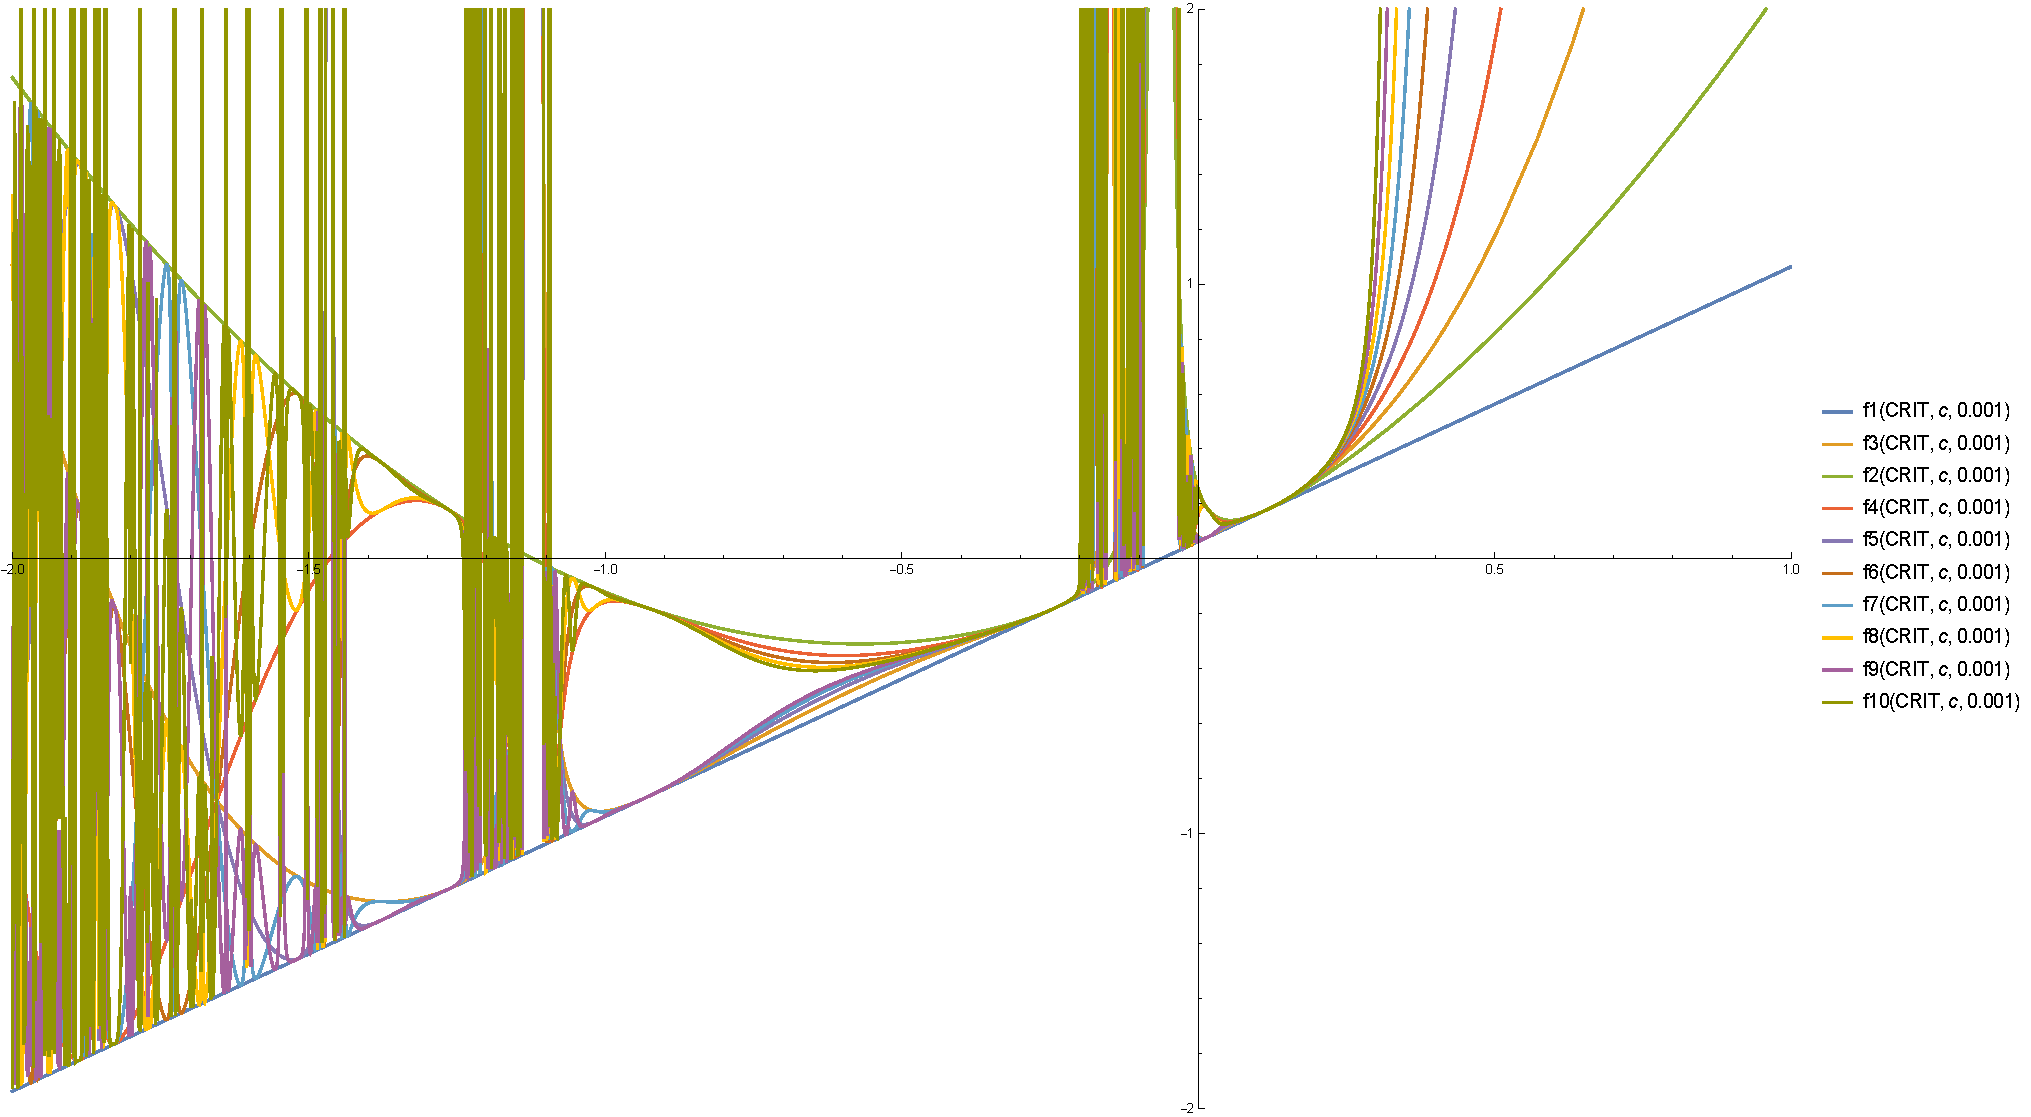
\includegraphics[width=\textwidth]{./img/pert}
					\caption{Orbit diagram of $x^2 + c + \frac{.001}{x^2}$}
					\label{pert}
			\end{subfigure}%
			\begin{subfigure}[b]{0.5\textwidth}
					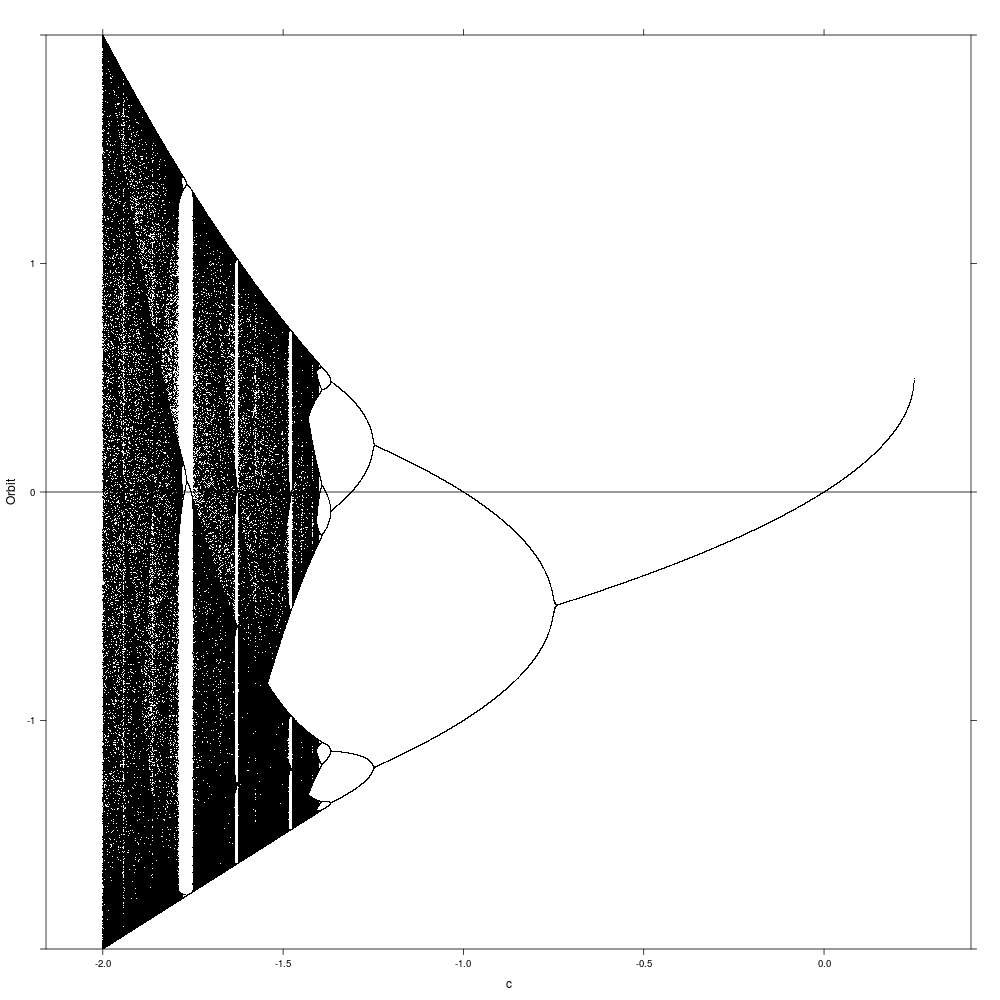
\includegraphics[width=\textwidth]{./img/orig}
					\caption{Orbit diagram of $x^2 + c$}
					\label{stand}%
			\end{subfigure}
			\caption{Orbit diagrams of the perturbed system and the original system}\label{fig:orbits}
		\end{figure}

		Now that we have established that the behavior of the critical orbit helps determine the behavior of the system, we can perform a few numerical experiments to discover where the dynamics of the perturbed system varies from the dynamics of the original quadratic map $Q_c (x) = x^2 + c$. As previously discussed, a standard analysis of the behavior of the critical orbit is to create an orbit diagram as shown in Figure \ref{pert} and Figure \ref{stand}. Immediately we can see some major differences between the behavior of the two families. One of the most notable differences is on the parameter interval $c\in (-.25, .05)$ (magnifications of which are shown in Figures \ref{pertz2} and \ref{pertz1}).

		The following section will discuss the behavior of the system for $c$ intervals which are either straightforward or analogous to the behavior of the original quadratic map. Subsequent sections will then describe some of the behavior where the perturbed  map acts quite differently than the standard map, providing some instances of interesting critical orbit behavior. Since $\beta = .001$ is fixed from this point forward, we will refer to $f_{c, \beta = .001}$ as $f_{c}$.

		\begin{figure}[h]
			\centering
			\begin{subfigure}[b]{0.5\textwidth}
					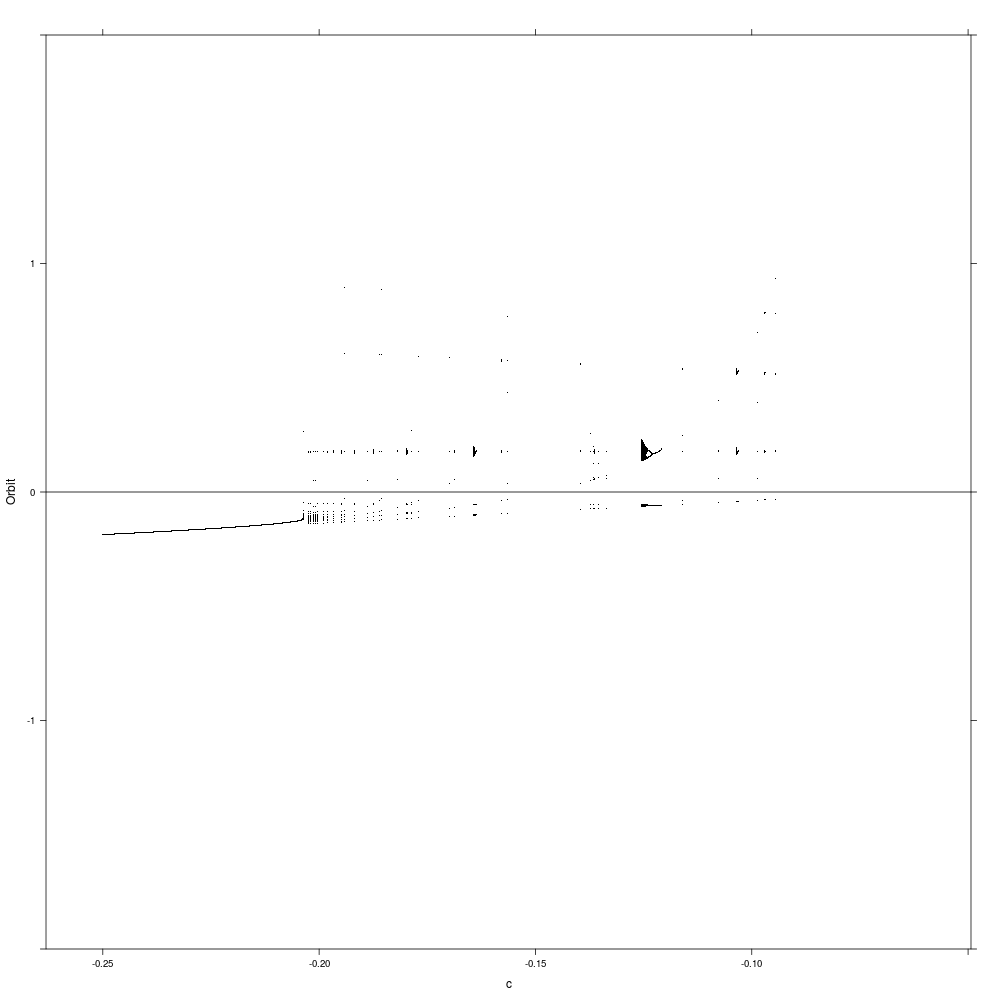
\includegraphics[width=\textwidth]{./img/pertzoom2}
					\caption{$c\in (-.25, -.062456)$}
					\label{pertz2}
			\end{subfigure}%
			\begin{subfigure}[b]{0.5\textwidth}
					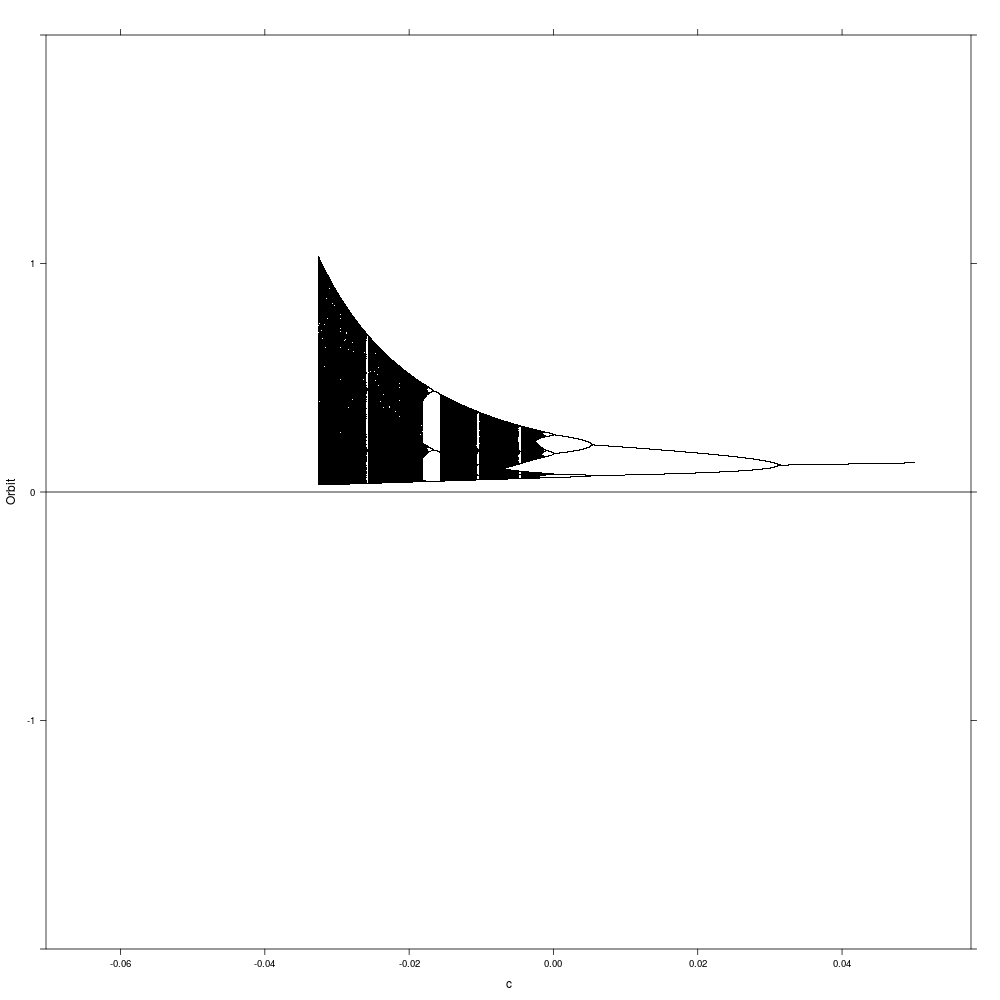
\includegraphics[width=\textwidth]{./img/pertzoom1}
					\caption{$c\in (-.062456, .05)$}
					\label{pertz1}%
			\end{subfigure}
			\caption{Zooms of the perturbed system's orbit diagram}\label{fig:orbits2}
		\end{figure}

	\section{Intervals of Understood Behavior} \label{res:understood}

	A cursory review of the orbit diagrams in Figure \ref{fig:orbits} reveals that the overall behavior of the systems seems to be quite similar, with many regions being nearly identical while some are entirely different. This section will focus on the former type of parameter intervals, briefly covering regions were the dynamics are fairly straightforward/similar to well known behaviors. In addition to the numerical bounds for each interval, we will include the special parameter names with orbit codings which will be introduced in the next section.

	Note that Figure \ref{fig:giters} provides graphical iteration of the positive critical point for most of the parameter values described below. These images may prove useful when trying to visualize how the system is changing at each parameter value.

	\underline{$c > .24604 \approx s_1^r$}

	For $c > .24604$, $f_c (x)$ behaves in a very similar manner to $Q_c (x)$ for $c > .25$ in that the plot is entirely above the reference line, as shown in Figure \ref{esc}. In both cases, all orbits escape because the function has no fixed points or periodic behavior so there is nothing to prevent all orbits from escaping to $\infty$ (hence the white space in our orbit diagrams). This interval of universal escape ends when the $f_c (x)$ undergoes a saddle node bifurcation at $c \approx .24604 \approx s_1^r$. This change is analogous to the saddle node of $Q_c (x)$ which occurs at $c = .25$. 

	\begin{figure}
		\centering
		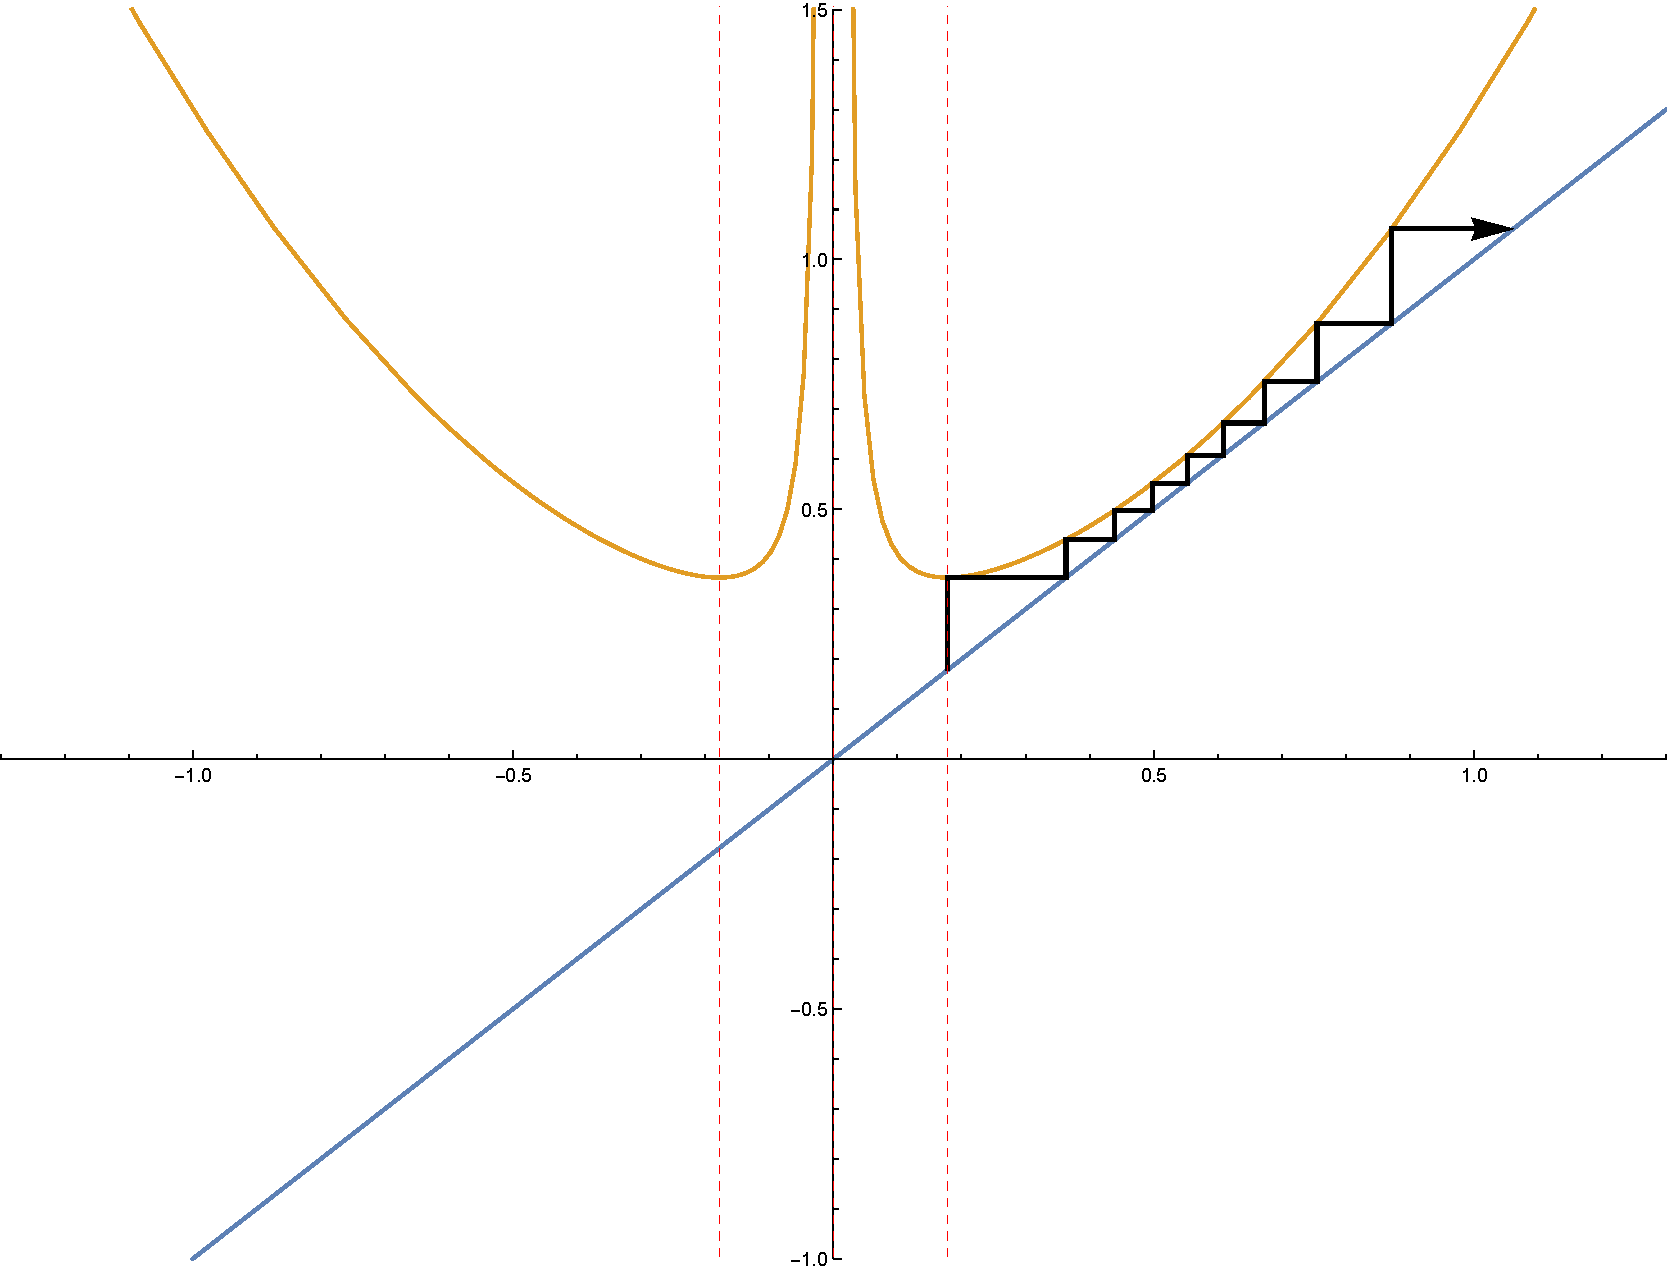
\includegraphics[width=.75\textwidth]{./img/plot03}
		\caption{Graphical iteration of the positive critical point under $x^2 + .3 + \frac{.001}{x^2}$, showing escape}
		\label{esc}
	\end{figure}

	

	\underline{$c \in (-.03255, .24604) \approx (h_2^{CLP_c}, s_1^r)$}

	Following the saddle node bifurcation and until $c \approx -.035$, the perturbed system seems to be going through the standard period doubling route to chaos that is similar to the behavior exhibited by $Q_c (x)$ for $c \in (-2,.25)$. Figure \ref{fig:perdub} shows a zoom of the perturbed map over $c\in (-.35, .05)$ along side the orbit diagram for $Q_c (x)$. While the exact shapes of the two images are slightly different, it is readily apparent that the two systems are exhibiting nearly identical behavior, that is to say that they appear to be topologically equivalent. For example, we can trace out the sequence of period doublings from 1 to 2 to 4 and so on, as well as match other windows (especially the period three which is very clear on both diagrams). The reason for this similarity is that on this parameter interval, the bimodal map $f_c (x)$ is actually acting as a unimodal map because the entire curve is above 0, meaning that all orbits are acting on only the right portion of the curve after at most one iterate. Additionally, this unimodal map has a very similar shape to that of the quadratic map, causing a similar sequence of bifurcations to occur. Thus this interval has been reduced to already known results and we expect that the methods from the study of the $Q_c (x)$ map would be able to describe the behavior observed over this parameter interval.

	\begin{figure}[h]
		\centering
		\begin{subfigure}[b]{0.48\textwidth}
				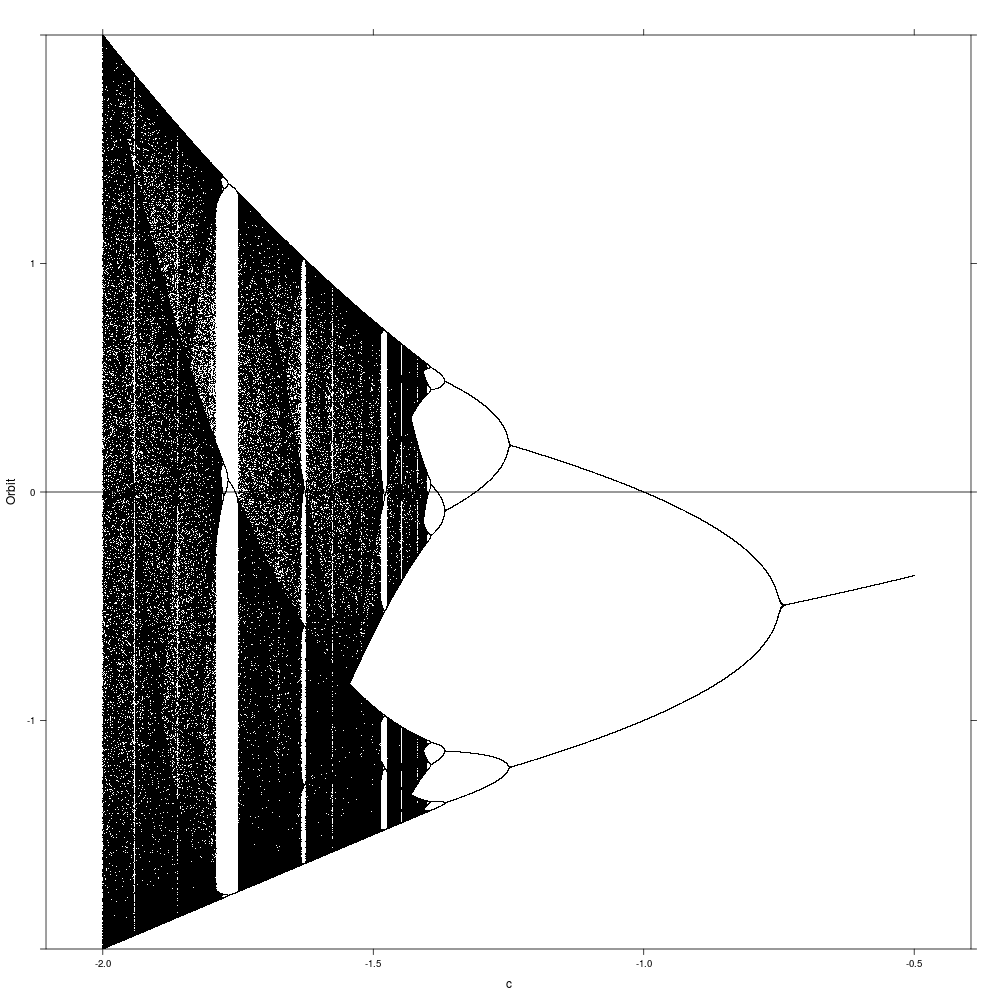
\includegraphics[width=\textwidth]{./img/stdperdub}
				\caption{Orbit Diagram for $Q_c (x)$ where $c\in (-2, -.5)$}
		\end{subfigure}
		\begin{subfigure}[b]{0.48\textwidth}
				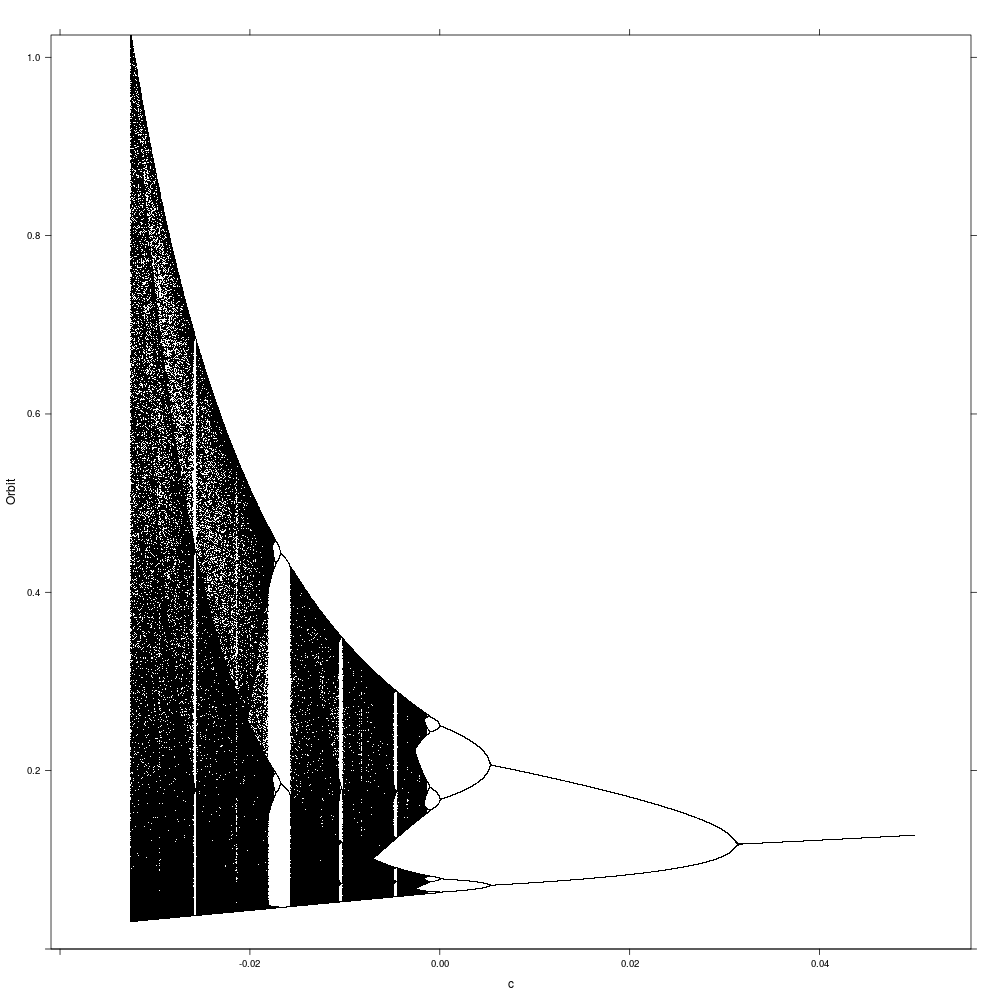
\includegraphics[width=\textwidth]{./img/pertperdub}
				\caption{Orbit Diagram for $f_c (x)$ where $c\in (-.035, .05)$}
		\end{subfigure}%
		\caption{Orbit diagrams of the original system and the perturbed system}\label{fig:perdub}
	\end{figure}

	\underline{$c\in (-.0632456, -.03255) \approx (z_1^{C0}, h_2^{CLP_c})$}

	For $c < -.03255$, the critical value first escapes by mapping just to the right of the right hand fixed point and then continuing to infinity. Thus the dynamics on this interval would be very similar to the dynamics of $Q_c (x)$ for $c < -2$ where the critical orbit escapes leaving a Cantor set of points which stay bounded. Again similar techniques from the quadratic map study would likely be able to prove that the dynamics on this remaining Cantor set would exhibit chaotic behavior when considered under a conjugacy with the Shift Map on two symbols. As $c$ continues to drop, this first iterate of the critical value is mapped higher and higher up the singularity around 0 until $c \approx -.0632456 \approx z_1^{C0}$ where $f_c (C) = 0$ as we see below:
	\[
		f_c (C) = 0 \Ra \left (\beta^{\frac{1}{4}}\right)^2 + c + \frac{\beta}{\left (\beta^{\frac{1}{4}}\right)^2} = 0 \Ra c = -2 \beta^{\frac{1}{2}} \Ra c = -2 (.001)^{\frac{1}{2}} \Ra c \approx -.0632456 \approx z_1^{C0}
	\]
	Thus at the parameter value $z_1^{C0}$ the $n^{th}$ iterate of the critical point maps directly to $\infty$ for $n > 1$.

	\underline{$c\in (-.092495, -.0632456) \approx (h_2^{CLP_c}, z_1^{C0})$}

	As $c$ decreases from $z_1^{C0}$, the second iterate of the critical point moves down the left side of the singularity until the parameter value $c \approx -.092495$ which is the point where the first iterate is small enough such that the second iterate is exactly the right hand fixed point $P_c$. Once the second iterate lands below $P_c$, the behavior is no longer similar to the behavior of $Q_c (x)$ for $c < -2$. Again refer to Figure \ref{fig:giters} for graphical iteration depicting most of the changes discussed here

	\underline{$c\in (-.241073, -.092495) \approx (p_1^{-C}, h_2^{CrP_c})$}

	This interval is the subject of the following sections where it will be described in detail.

	\underline{$c \in (-2.1, -.241073) \approx (h_2^{ClP_c},p_1^{-C})$}

	In this interval, $f_c$ again acts in a similar manner to the $Q_c (x)$ map because whenever the critical orbit stays far enough away from the singularity, the global geometry of the curve has more influence than the singularity. However we do note several significant deviations from the $Q_c (x)$ dynamics, most notably where the map ``should'' undergo a period doubling bifurcation. Instead, the $f_c (x)$ orbit diagram seems to be filling an interval of orbit values, indicating more complicated behavior. Additionally, the orbit diagram isn't nearly as well filled in at other points (even though the same number of iterates were plotted in either case). This is likely due to the many complicated ways by which points may escape through the ``trap door'' near $x=0$. Further study would be required to fully understand the behavior on this interval and appreciate its similarity/dissimilarity to $Q_c (x)$.

	\underline{$c < -2.1 \approx h_2^{ClP_c}$}

	On this interval, the critical orbit again escapes because its second iterate lands to the right of the right hand fixed point $P_c$. Again the dynamics on this interval would be similar to that of the $Q_c (x)$ map for $c < -2$ where there would be a Cantor set of points remaining. Here though, instead of two preimages of every escaping interval as we have with $Q_c (x)$, $f_c (x)$ would have four preimages of the escaping interval due to its bimodal shape. Thus instead of the middle thirds Cantor set for $Q_c (x)$, we would likely have a middle ``four ninths'' Cantor set of points which do not escape. The dynamics of the points in this set should be conjugate to the shift map on four symbols.

	\section{Orbit Codings}

	Before introducing our results, we will discuss one final analytical technique which is critical to understanding the results presented in the following sections. It is common in the study of one-dimensional dynamical systems to partition the the domain/codomain into a series of intervals. Once such a partition has been established, we can then encode orbits with a sequence of symbols determined by which partition each iterate maps to. The reason why this is useful is because we can look at the coding of a some orbit, say the critical orbit, and keep track of changes in that coding as the parameter set changes. Typically when such a coding change occurs, the system has undergone some kind of shift as we moved from one parameter value to another. Therefore, orbit codings provide a simple numerical mechanism for detecting behavioral transitions. For parameter values within our interval of interest, we will impose the following partitioning for our system:

	\begin{figure}
		\centering
		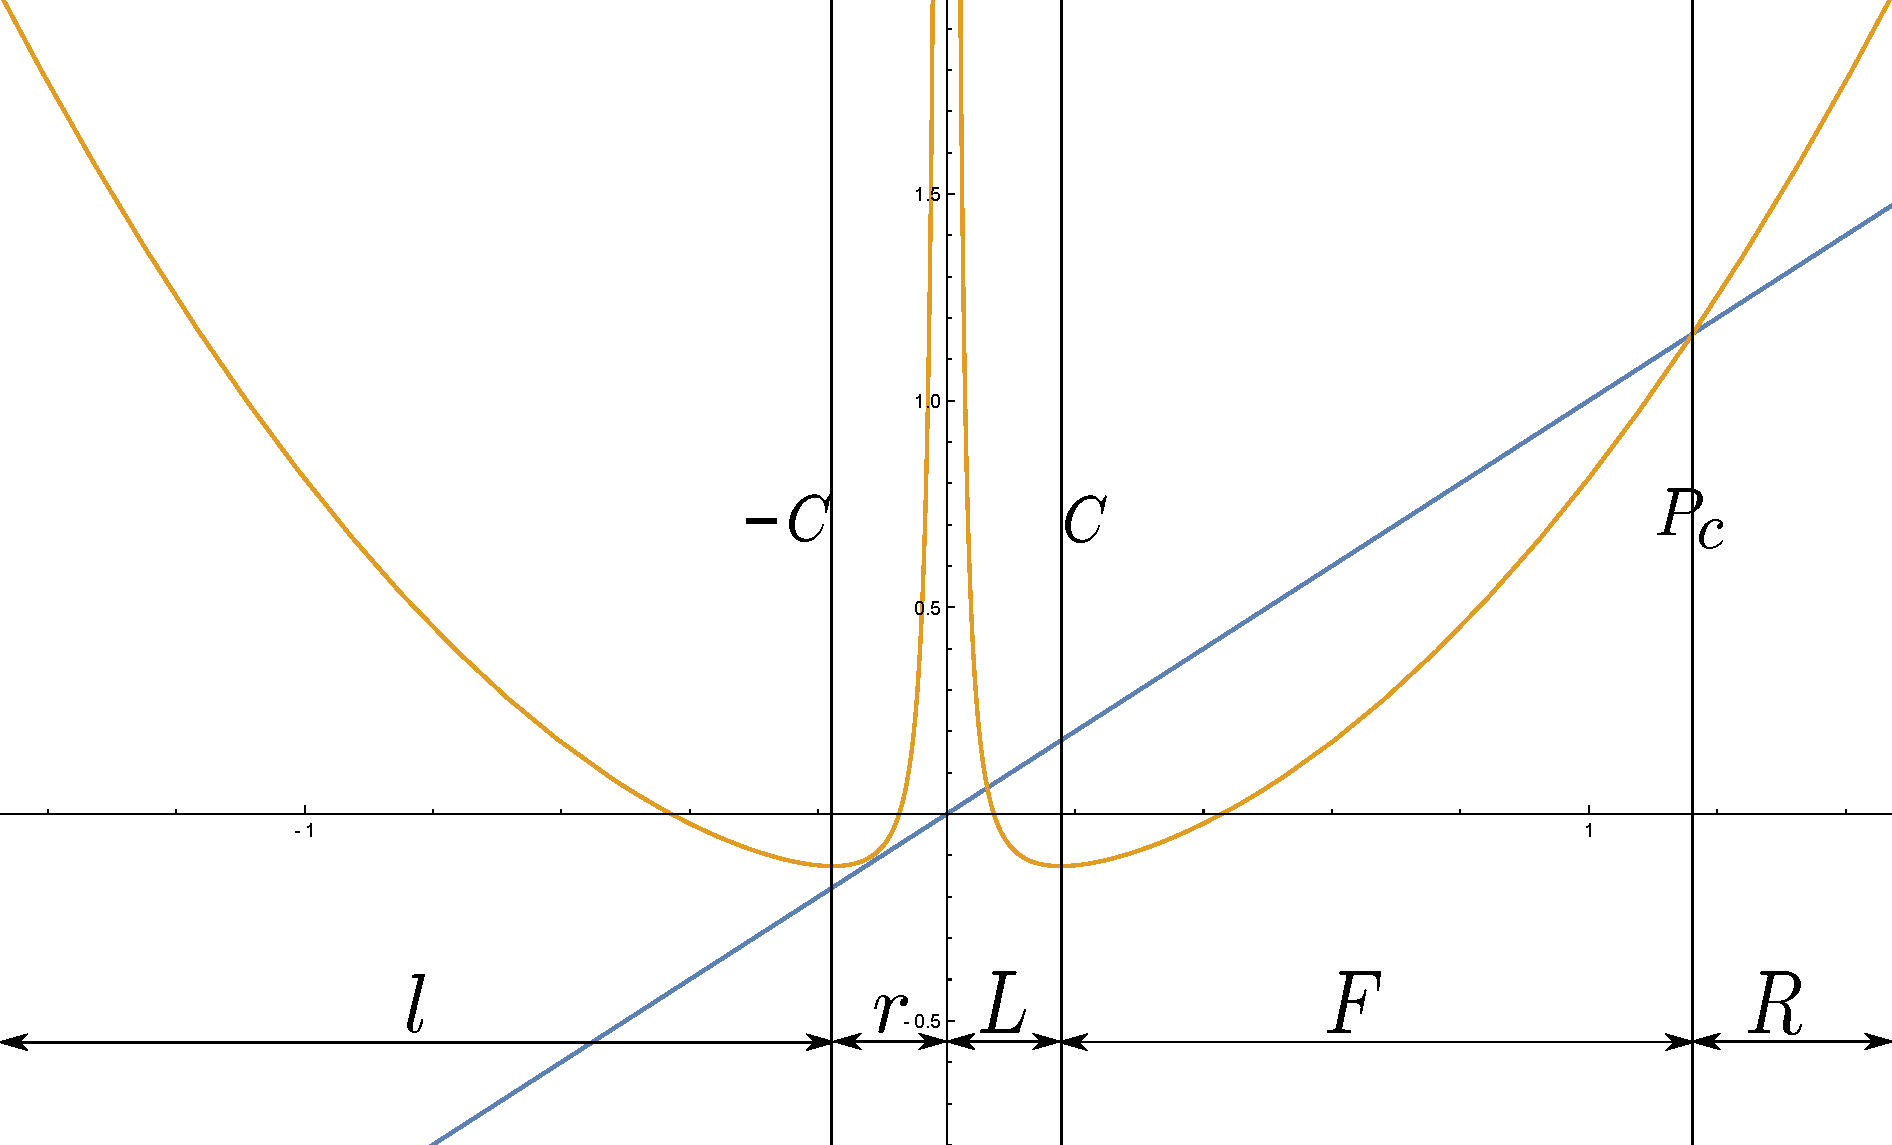
\includegraphics[width=.75\textwidth]{./img/codings.pdf}
		\caption{A partitioning of the domain of the map $f_c (c) = x^2 + c + \frac{.001}{x^2}$}
		\label{coding}
	\end{figure}

	\begin{itemize}
		\item Let $C$ be the positive critical point such that $C = + \beta^{\frac{1}{4}} = .001^{.25} \approx 0.177827$. $-C$ will simply denote the negative critical point.
		\item Let $P_c$ be the right most fixed point (when it exists) which is given by solving for the maximum $c$ value which satisfies $f_c (x) = x$. The curve in $c$ space produced by the solution of this system is shown in Figure \ref{pcplot}.
		\item $R$: Corresponds to $\{x | x\in (P_c, \infty)\}$. Over this interval, $f_c (x)$ is always increasing with respect to $x$ for all $c$. Additionally, once any iterate lands in this interval escape is inevitable.

		\item $F$: Corresponds to $\{x | x\in (C, P_c)\}$. Over this interval, $f_c (x)$ is increasing with respect to $x$ for all $c$.

		\item $L$: Corresponds to $\{x | x\in (0, C)\}$. Over this interval, $f_c (x)$ is decreasing with respect to $x$ for all $c$.

		\item $r$: Corresponds to $\{x | x\in (-C, 0)\}$. Over this interval, $f_c (x)$ is increasing with respect to $x$ for all $c$.

		\item $l$: Corresponds to $\{x | x\in (-\infty, -C)\}$. Over this interval, $f_c (x)$ is decreasing with respect to $x$ for all $c$.

		\item In addition to the above intervals, we will also define codes corresponding to boundary points: 0, $C$, $-C$, $P_c$, and $\infty$ where $C$ and $-C$ are the critical points of our system and $P_c$ is the rightmost fixed point.
	\end{itemize}

	\begin{figure}
		\centering
		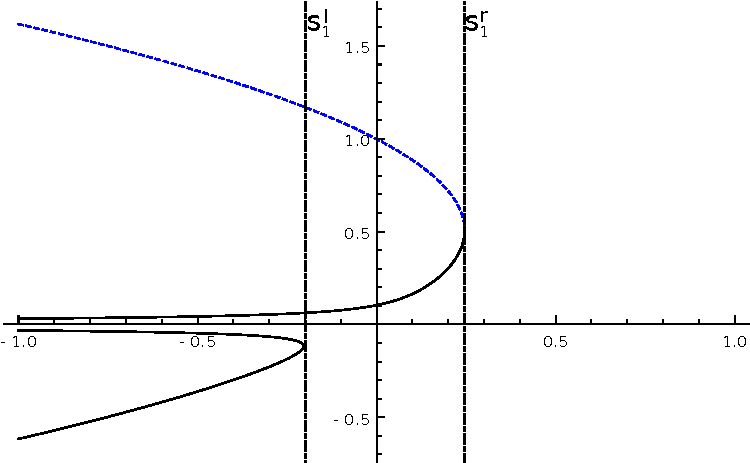
\includegraphics[width=.75\textwidth]{./img/pc}
		\caption{Plot of all the fixed points with respect to $c$, $P_c$ is the max such value for any $c$ (shown in a dashed line)}
		\label{pcplot}
	\end{figure}

	Note that the intervals $l$, $r$, and $L$ are invariant under changes in our parameter $c$ (because the critical points are not a function of $c$) while $F$ and $R$ are dependent on the value of $P_c$ which depends on $c$. See Figure \ref{coding} for a graphical representation of these intervals. Throughout the remainder of this paper, we will make heavy use of critical orbit codings of the form $C\alpha_1\alpha_2\cdots\alpha_n$. As mentioned above, keeping track of such codings is useful because they can easily detect when some $i^{th}$ iterate moves from one interval to another. This is significant not only because it could mark the difference between bounded and unbounded orbits, but because between any two distinct codings, there are the significant values $-C$, $0$, $C$, and $P_c$. Thus, since our map varies continuously with respect to both $c$ and $x$ (see Proposition \ref{contin}), if $\alpha_i$ changes from one coding at the value $c_1$ to another coding at $c_2$, we are guaranteed by the Intermediate Value Theorem that the $i^{th}$ iterate must have taken on an intermediate value according to Table \ref{trans} (note that all transitions are transitive such that a transition $l \ra L$ implies $l \ra r$ and $r \ra L$).
	
	\begin{table}[h]
		\centering
		\begin{tabular}{|c|c|}
		\hline Coding Transition & Guaranteed Intermediate Value\\
		\hline $l \leftrightarrow r$ & $-C$\\
		\hline $r \leftrightarrow L$ & $0$\\
		\hline $L \leftrightarrow F$ & $C$\\
		\hline $F \leftrightarrow R$ & $P_c$\\
		\hline
		\end{tabular}
		\caption{Summary of coding transitions and their implications}
		\label{trans}
	\end{table}

	\section{Parameter Interval of Interest and Naming Conventions}

	The goal of subsequent sections is to introduce the results concerning the behavior of the critical orbits of $f_c$ within the parameter interval $ (-.25, -.062456)$ as discussed in Section \ref{res:understood}. Before doing so, we will briefly introduce some naming conventions which will aid our description of the behavior in this interval:

	In addition to the codes defined in Section 3.3, we will adopt the following naming conventions for simplicity:
	\begin{itemize}
		\item Let $\inte{a}{b} = (\min\{a,b\}, \max\{a,b\})$ such that $\inte{a}{b}$ is simply the interval between $a$ and $b$ where $a > b$ or $b > a$.
		\item Let $h_n$, $p_n$, $z_n$ be parameter values such that $f^n_{h_n} (C) = P_c$ (corresponding to a homoclinic parameter value), $f^n_{p_n} (C) = C$ (corresponding to a superattracting periodic orbit parameter value), and $f^n_{z_n} (C) = 0$ (corresponding to a prezero parameter value, see Section 4.3). Note that the solutions to these equations are typically not unique; thus we will refer to a specific parameter value with the coding of the critical orbit at that point by placing the coding at that parameter value in the superscript. For example, in Figure \ref{itright} we see graphical iteration of the critical point at the parameter value $\pr$ where we refer to the specific $h_2$ by listing the coding $CrP_c$.
		\item Let $s_n$ be a parameter value where the $n^{th}$ iterate goes through a saddle node bifurcation. We use an $l$ or an $r$ in the superscript to differentiate between the left lobe saddle and the right lobe saddle respectively. $s_1^l$ and $s_1^l$ are labeled in Figure \ref{pcplot}.
	\end{itemize}
	%This behavior is interesting because it forces the existence of some parameter neighborhood where all higher iterates of the critical orbit escape. As a consequence of Theorem \ref{sch}, if the critical point escapes, there can be no attracting periodic points at that parameter value.
\begin{figure}[h]
	\centering
	\begin{subfigure}[b]{0.5\textwidth}
			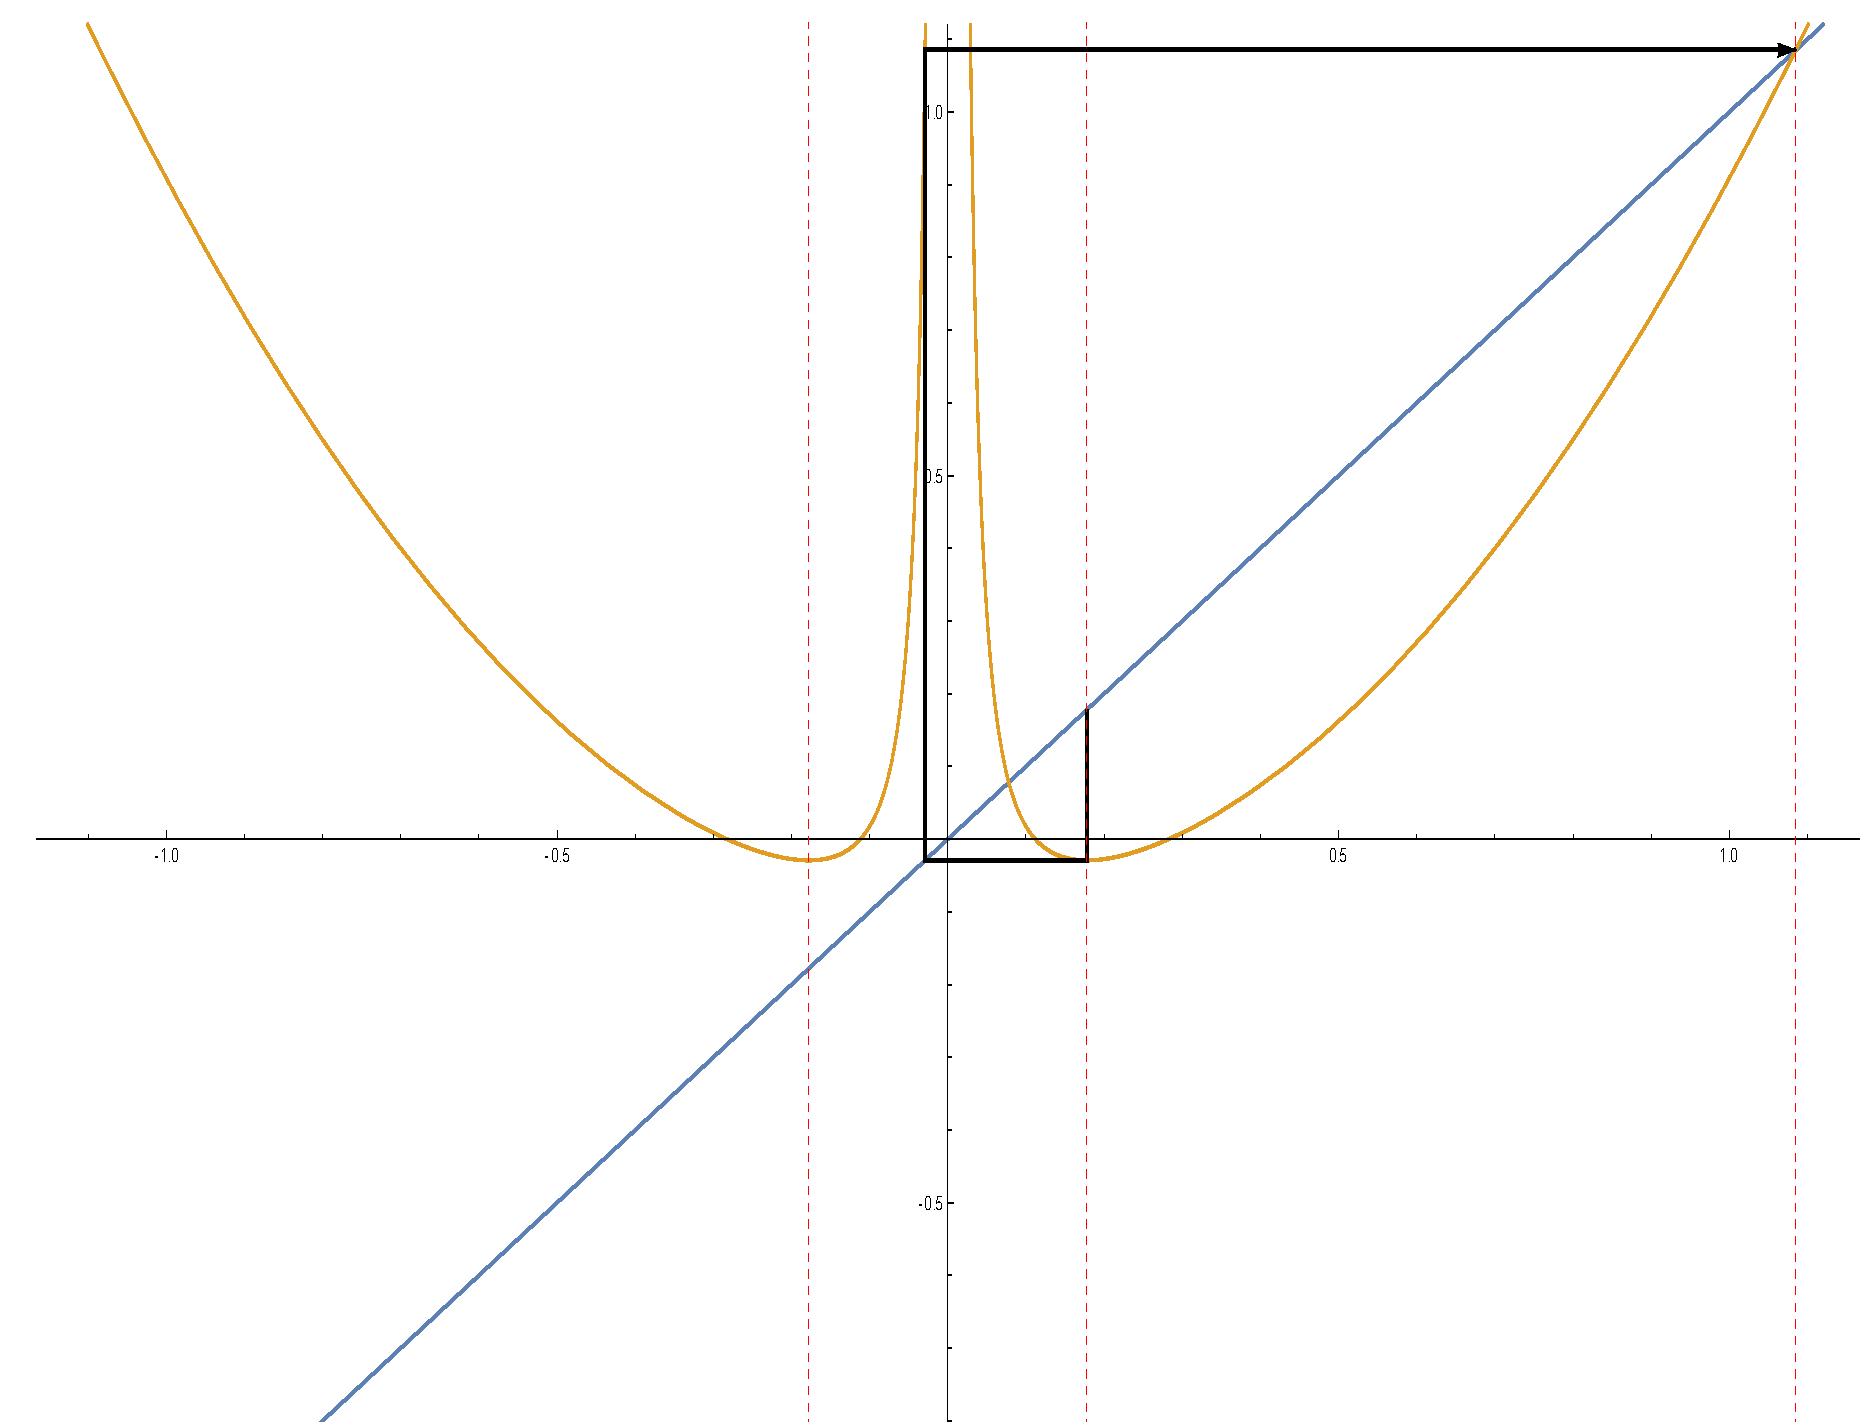
\includegraphics[width=\textwidth]{./img/c1}
			\caption{Graphical Iteration of $C$ at the parameter value $\pr$}
			\label{itright}
	\end{subfigure}%
	\begin{subfigure}[b]{0.5\textwidth}
			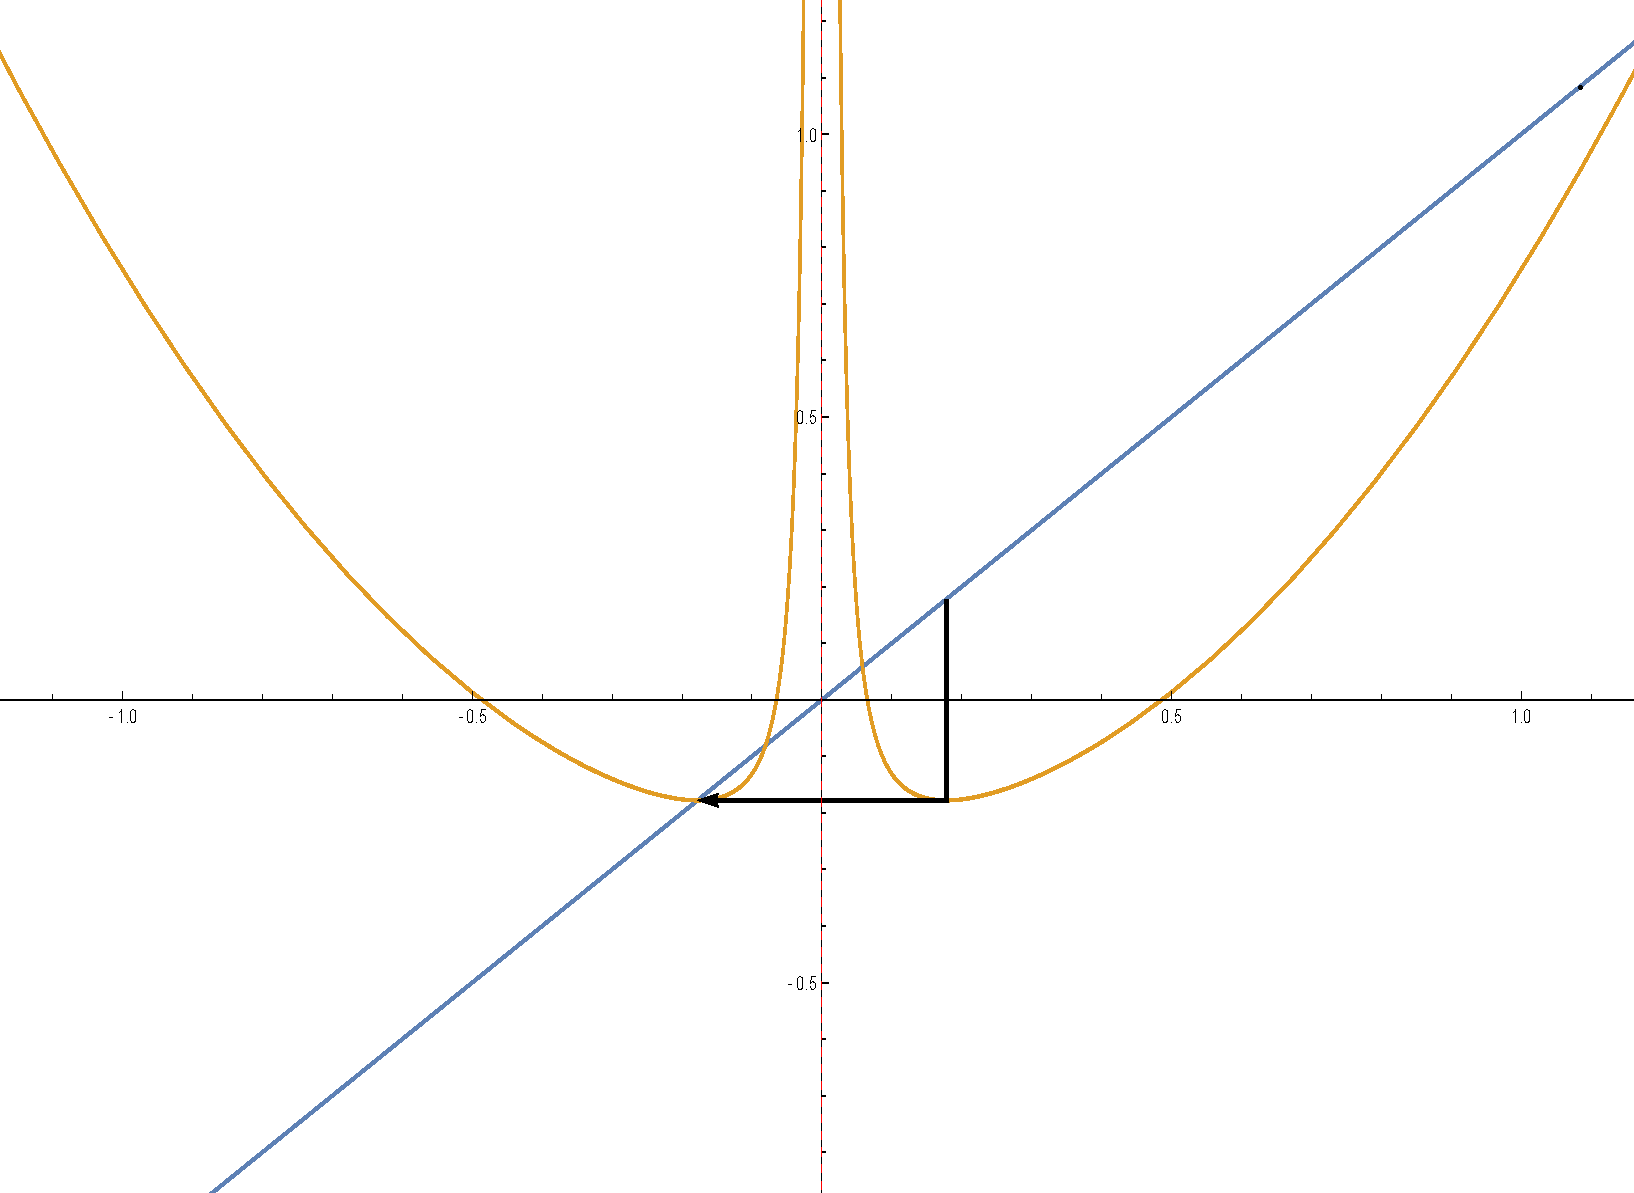
\includegraphics[width=\textwidth]{./img/c2}
			\caption{Graphical Iteration of $C$ at the parameter value $\pl$}
			\label{itleft}%
	\end{subfigure}
	\caption{Graphical Iteration at the key parameter values $\pr$ and $\pl$}\label{fig:cgi}
\end{figure}

A study of the orbit diagrams from the previous sections reveals that there are several ``key'' parameter values on the interval $ (-.241073, -.092395)$ which can be used to frame our discussion of the critical point behavior. The first, which we call $\pr$, occurs approximately at $-.092395$ and represents the first $c$-value for which the critical orbit stays bounded as $c$ is decreased from $z_1^{C0}$. See Figure \ref{itright} for graphical iteration at this parameter value. Additionally, this also happens to be the parameter value where the critical orbit is prefixed at the right hand fixed point, as the notation suggests. We will also call the right hand fixed point at this parameter value the ``primary homoclinic point'' for reasons which we will discuss in full in Section \ref{hcs}. The second significant parameter value is $\pl \approx -.241073$ and represents the point where the negative critical point $-C$ is fixed. See Figure \ref{itleft} for graphical iteration at this parameter value. Note that both of these parameter values yield critical orbits which are fixed after two and one iterates respectively. Thus for any positive integer $n$, $f^n_{\pl} (C) = -C$ and for $n > 1$, $f^n_{\pr} (C) = P_c$. This means that higher iterates must be constrained at these points, providing a structure will be exploited in the arguments to follow. Finally, we introduce the point $s_1^l \approx -.203$ which represents the point where the left lobe becomes tangent to the reference line and undergoes a saddle node bifurcation (as the notation suggests). This point is significant because the system seems to return to a behavior more like the original map $Q_c (x)$ for $c < s_1^l$ (as discussed in Section 3.2).


	\section{The Two Primary Accumulation Points}
This section will provide a visual overview of the results concerning the two primary sequences of special parameter values as we approach $s_1^l$ from the right and $\pr$ from the left. The following propositions from Chapter 4 summarize the accumulation that we are seeing in the figures to follow:

\begin{customthm}{\ref{homaccum}}
% On the interval $ (\pl, \pr)$, there is an accumulation of parameter values $p_n^{CrF^{n-2}C}$ and $z_n^{CrF^{n-2}0}$ for any integer $n \geq 2$ such that 
% \[
% z_n^{CrF^{n-2}0} < p_n^{CrF^{n-2}C} < z_{n+1}^{CrF^{n-1}0} < p_{n+1}^{CrF^{n-1}C}
% \]
% The numerics suggest that the accumulation will limit to the point $P_c$.
On the interval $ (\pl, \pr)$, there is an accumulation of parameter values $p_n$ and $z_n$ for any integer $n \geq 2$ where the critical orbit has coding $CrF^{n-2}C$ and $CrF^{n-2}0$ respectively. These parameter values have the ordering
\[
z_n < p_n < z_{n+1} < p_{n+1} < \cdots < h_2^{CrP_c}
\]
\end{customthm}

\begin{customthm}{\ref{sadaccum}}
% On the interval $ (\pl, \pr)$, there is an accumulation of parameter values $p_n^{Cr^{n-1}C}$, $z_n^{Cr^{n-1}0}$, and $h_n^{Cr^{n-1}P_c}$ for any integer $n \geq 2$ such that 
% \[
% z_{n+1}^{Cr^{n}0} < p_{n+1}^{Cr^{n}C} < h_{n+1}^{Cr^{n}P_c} < z_n^{Cr^{n-1}0} < p_n^{Cr^{n-1}C}  < h_n^{Cr^{n-1}P_c}
% \]
% The numerics suggest that the accumulation will limit to the point $s^l_1$.
On the interval $ (\pl, \pr)$, there is an accumulation of parameter values $p_n$, $z_n$, and $h_n$ for any integer $n \geq 2$ where the critical orbit has coding $Cr^{n-1}C$, $Cr^{n-1}0$, and $Cr^{n-1}P_c$ respectively. These parameter values have the ordering
\[
p_1^{-C} < \cdots < z_{n+1} < p_{n+1} < h_{n+1} < z_n < p_n < h_n
\]
\end{customthm}

Chapter 4 will introduce the proofs of these propositions; the remainder of this section is devoted to developing some graphical intuition as to how these accumulations propagate. Additionally these figures will serve as a useful reference when reading the proofs of the following chapter.  First, Figure \ref{hqorb} shows a large zoom of the Orbit Diagram for the parameter interval $ (\pl, \pr)$. Labeled on this figure are several of the $p_n$ values described in the above propositions with their coding. Based on a glance of this image, there seems to be some sort of limiting behavior as we approach either side of the parameter interval.

Next, Figure \ref{hqcplot} shows a plot of $f_c^1 (C)$, $f_c^2 (C)$, and $f_c^3 (C)$ where we are varying our parameter $c$ and looking at how each iterate of the critical point is changing (note that this plot is in the same space as the Orbit Diagram). On this plot we again show the coding intervals and label several of the accumulating parameter values as we approach $\pl$ from the right and $\pr$ from the left. Hopefully this image provides some sense as to where the special parameter values come from: in this space, they are simply the parameter values of intersections of some iterate of the critical point with some special value 0, $C$, or $P_c$, yielding a $z_n$, $p_n$, or $h_n$ respectively.

Figures \ref{fig:giters} and \ref{fig:giters2} provide graphical iteration of the right hand critical point at many of the key parameter values discussed so far. These figures are especially illuminating when considered as a sequence of images as $c$ decreases because one can gain an intuition as to how the system is evolving: as $c$ decreases from $\pr$, the second iterate moves down the curve from $P_c$ and in so doing, lands on several points which either cycle back to $C$ (giving a $p_n$), eventually land on 0 (giving a $z_n$), or eventually land on $P_c$ (giving an $h_n$). Again the codings of critical orbit at these parameter values can be constructed by following the graphical iteration.

Figure \ref{fig:iterh1} shows a sequence of images which depict the accumulation of $p_n$ and $z_n$ parameter values as we approach $\pr$. This sequence of images is a particularly good way to look at the accumulation because it is a visualization of the inductive proof of Proposition \ref{homaccum}. For any $n \geq 2$, $f^n_{\pr} (C) = P_c$ simply because the second iterate is fixed there (fixing all higher iterates). Then as we add higher iterates, we see that $f^{n+1}_{p_n} (C) < 0$, meaning that as the $n^{th}$ iterate makes its way to $P_c$ at $\pr$, it must cross the value $C$, giving a $p_n$, forcing the next iterate to be negative. In this manner, the proof of Proposition \ref{homaccum} constructs the sequence of $p_n$ and $z_n$ parameter values as required.

In a similar manner to Figure \ref{fig:iterh1}, Figure \ref{fig:iterh2} shows a sequence of images which depict the accumulation of $p_n$, $z_n$, and $h_n$ parameter values as we approach $\pl$. Again this is a great visualization of the proof of Proposition \ref{sadaccum}. For any $n \geq 1$, $f^n_{p_1^{-C}} (C) = -C$ simply because the first iterate is fixed there (fixing all higher iterates). Then as we add higher iterates, we see that $f^{n+1}_{z_n} (C) = \infty$, meaning that as the $n^{th}$ iterate makes its way to $-C$ at $p_1^{-C}$, it must cross the value $0$, giving a $p_n, h_n$, and then finally a $z_n$, forcing the next iterate to be $\infty$. This iterate must also make its way down to $-C$ so continuing in this manner, the proof of Proposition \ref{sadaccum} constructs the sequence of $p_n$, $h_n$, and $z_n$ parameter values as required.
\begin{sidewaysfigure}[ht]
	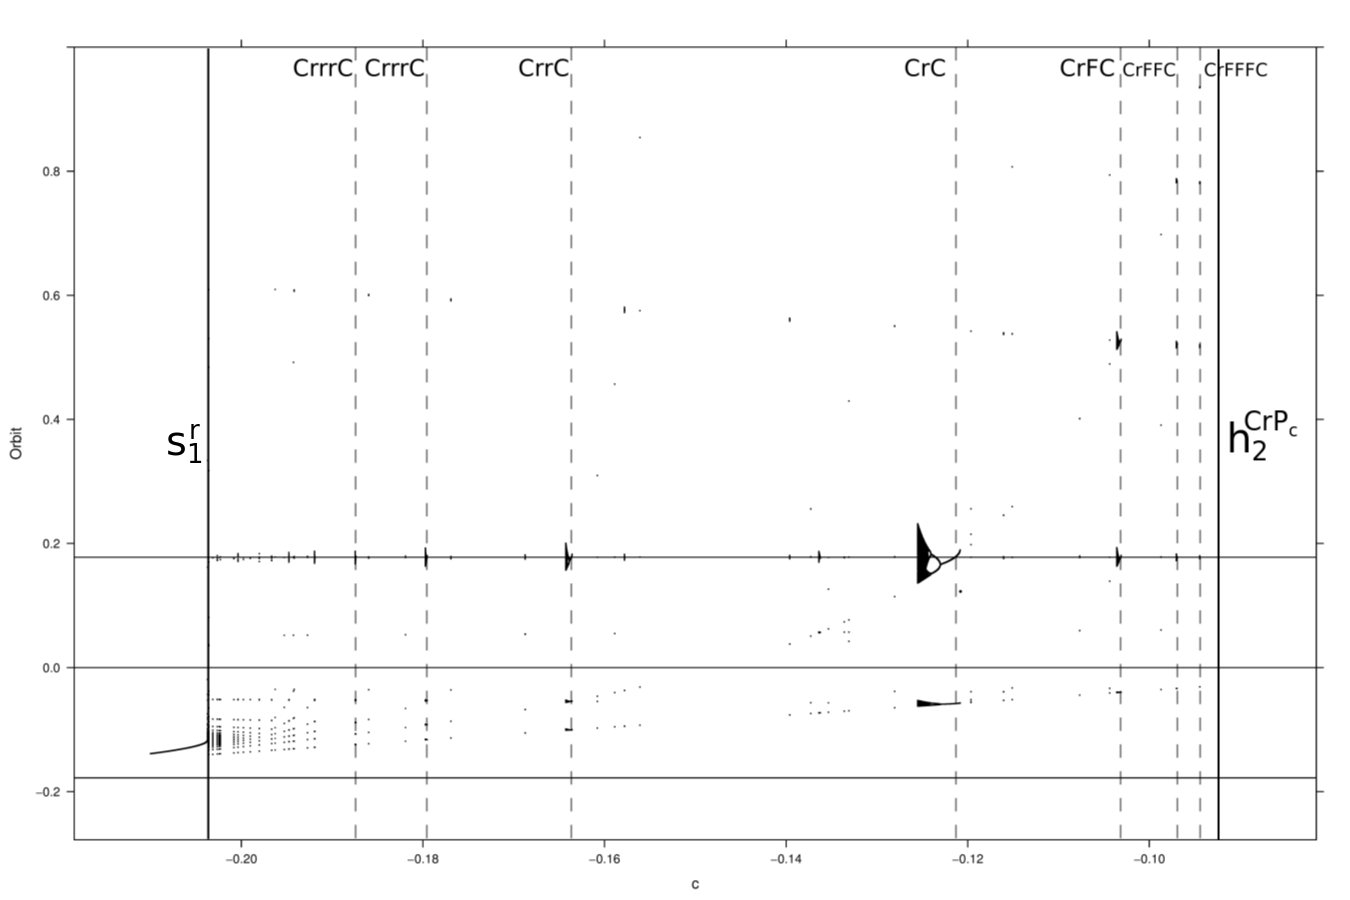
\includegraphics[width=\textheight]{./img/over.png}
	\caption{A high quality orbit diagram with several $p_n$ values and their codings indicated}
	\label{hqorb}
\end{sidewaysfigure}

\begin{sidewaysfigure}[ht]
	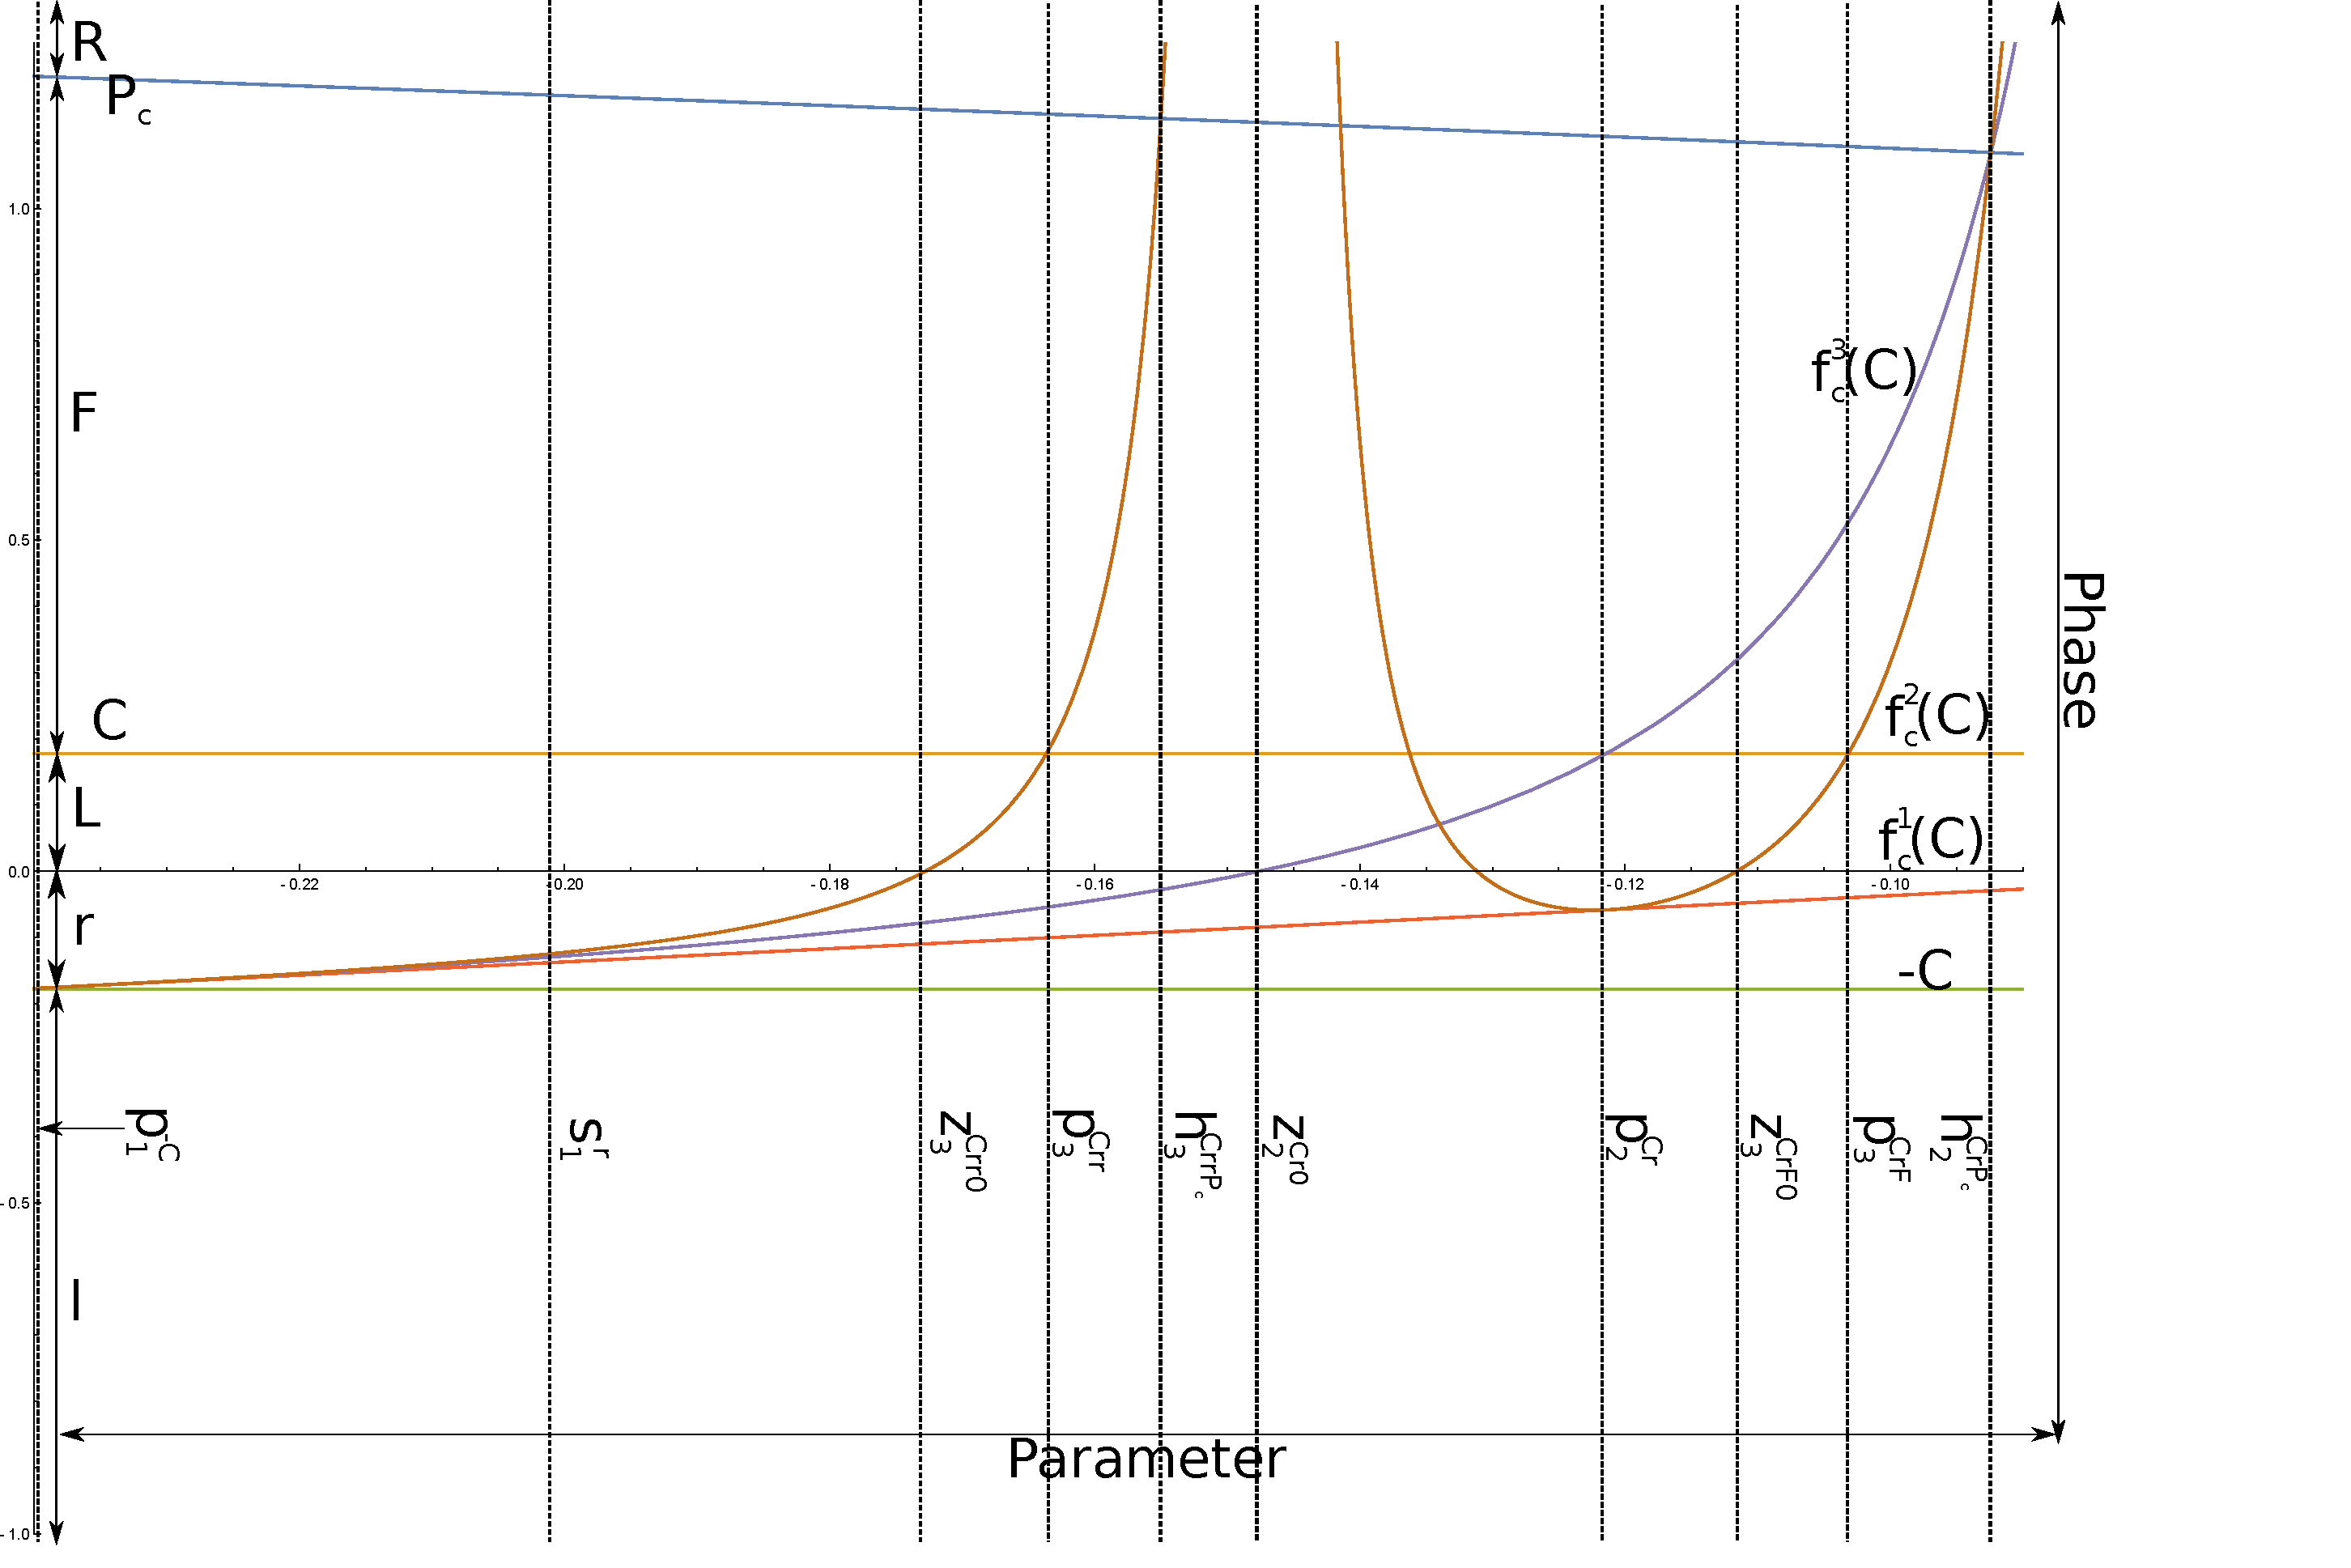
\includegraphics[width=\textheight]{./img/cs2}
	\caption{A plot of $f^1_c (C),f^2_c (C),f^3_c (C)$ in parameter$\times$phase space with the ``primary'' parameters labeled for $h_n,p_n,z_n$}
	\label{hqcplot}
\end{sidewaysfigure}

\begin{figure}[ht]
		\centering
		\begin{subfigure}[b]{0.3\textwidth}
				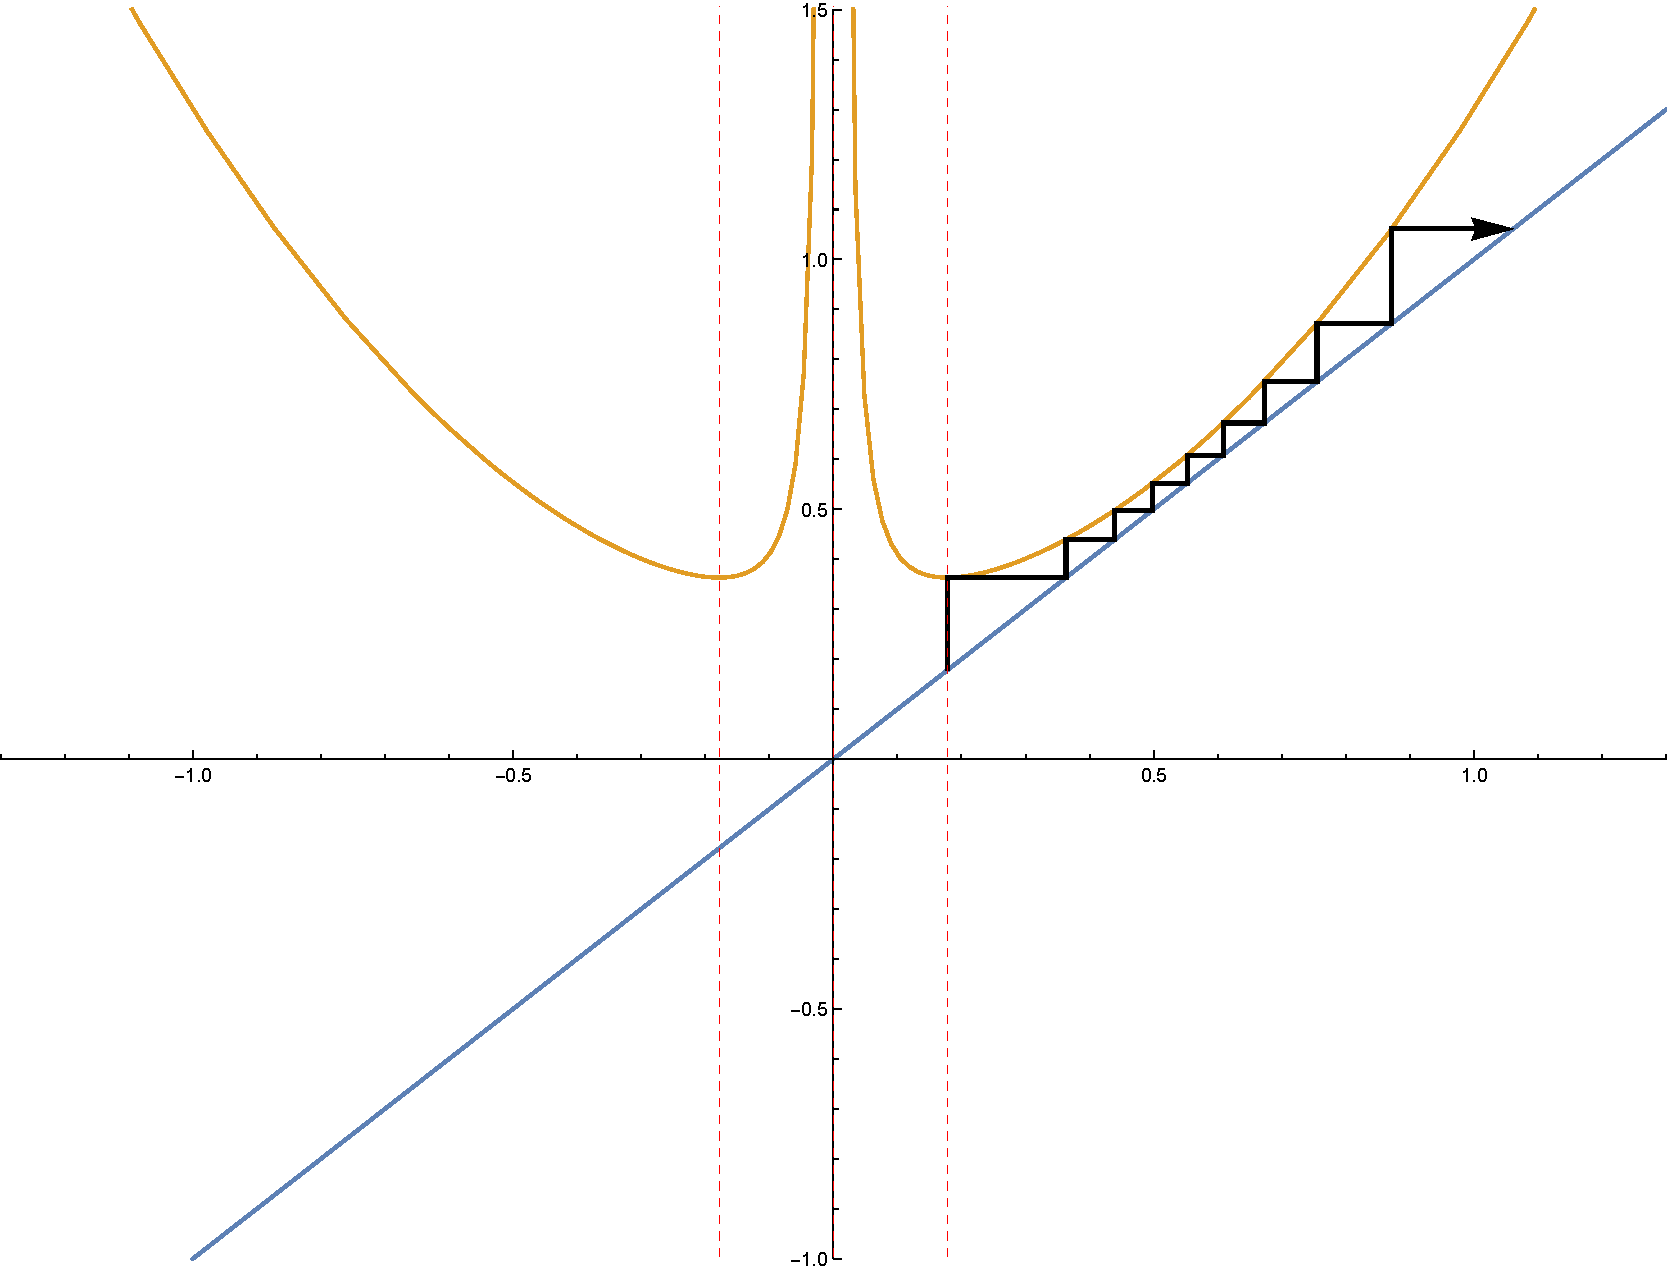
\includegraphics[width=\textwidth]{./img/plot03}
				\caption{$c \approx 0.3$}
		\end{subfigure}%
		\begin{subfigure}[b]{0.3\textwidth}
				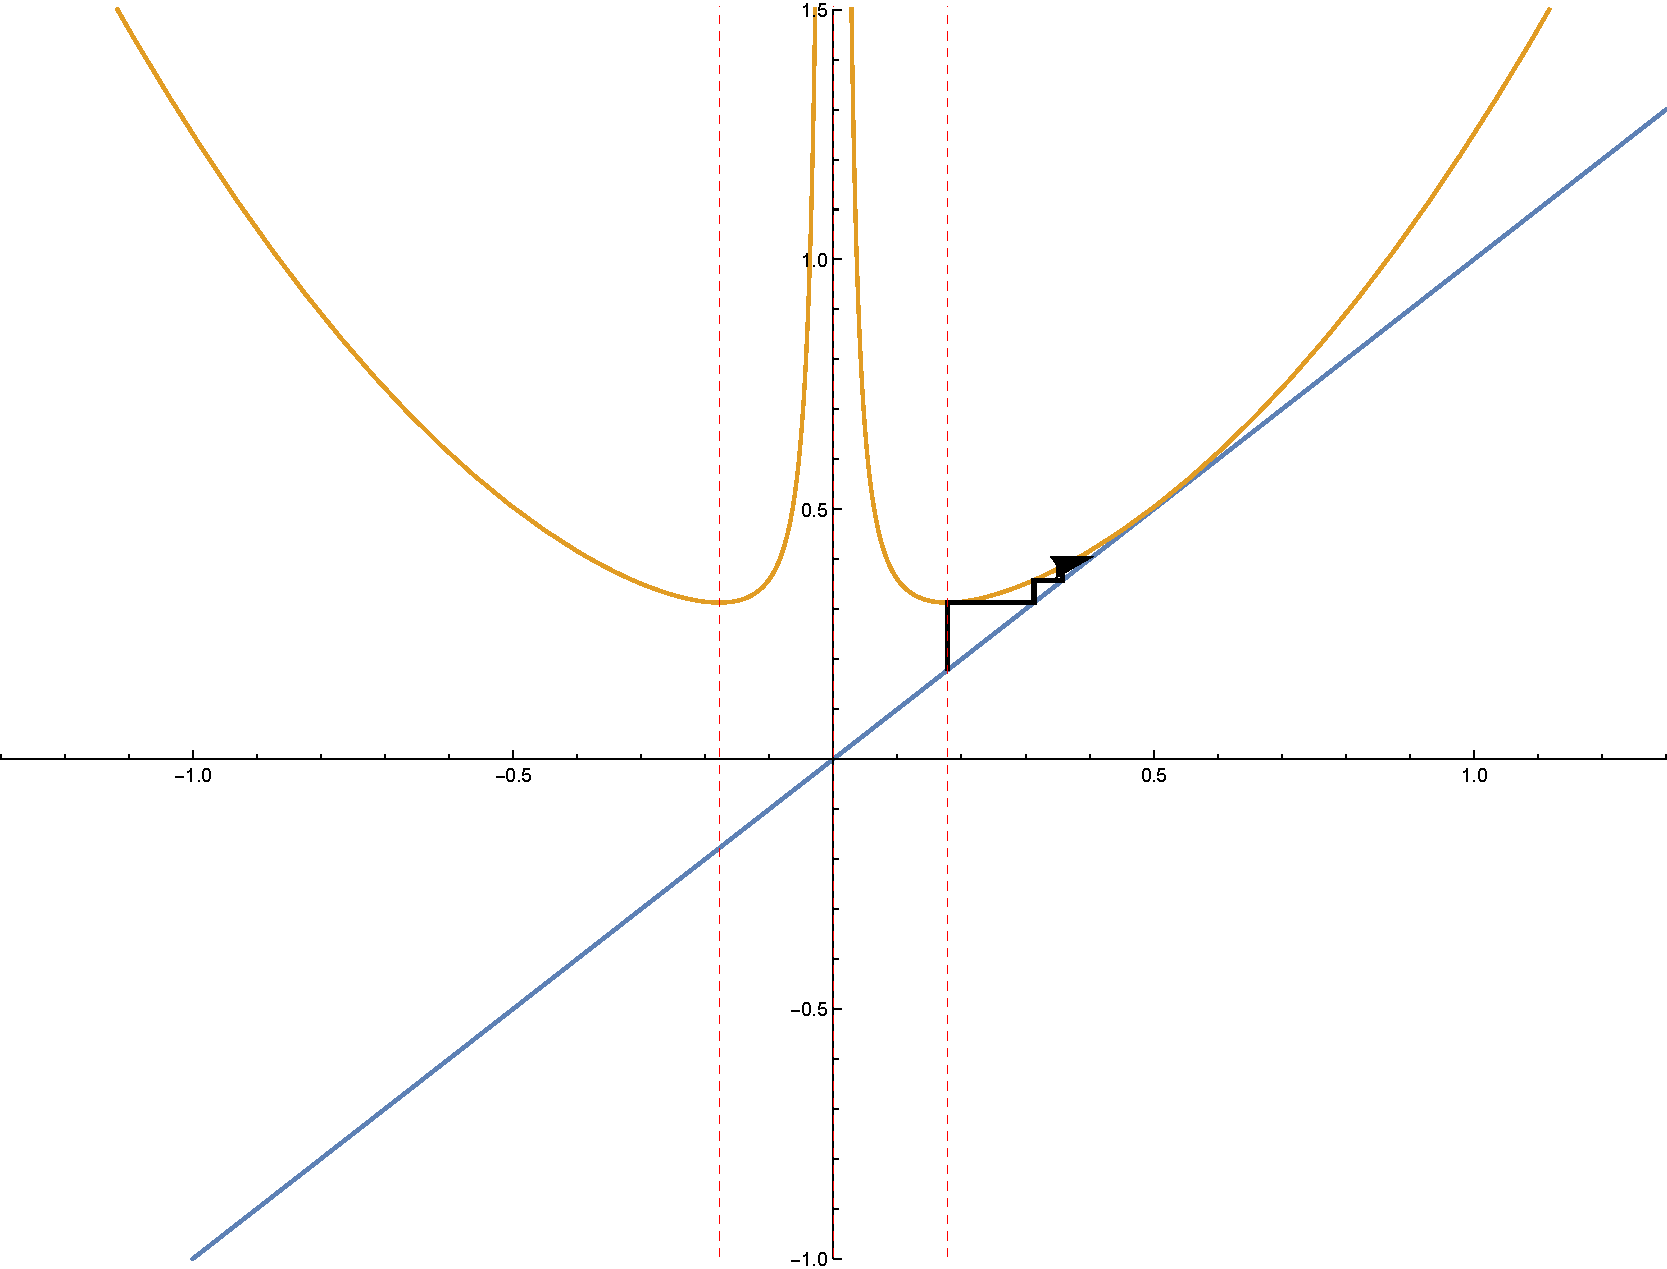
\includegraphics[width=\textwidth]{./img/plot025}
				\caption{$c \approx 0.24 \approx s_1^r$}
		\end{subfigure}
		\begin{subfigure}[b]{0.3\textwidth}
				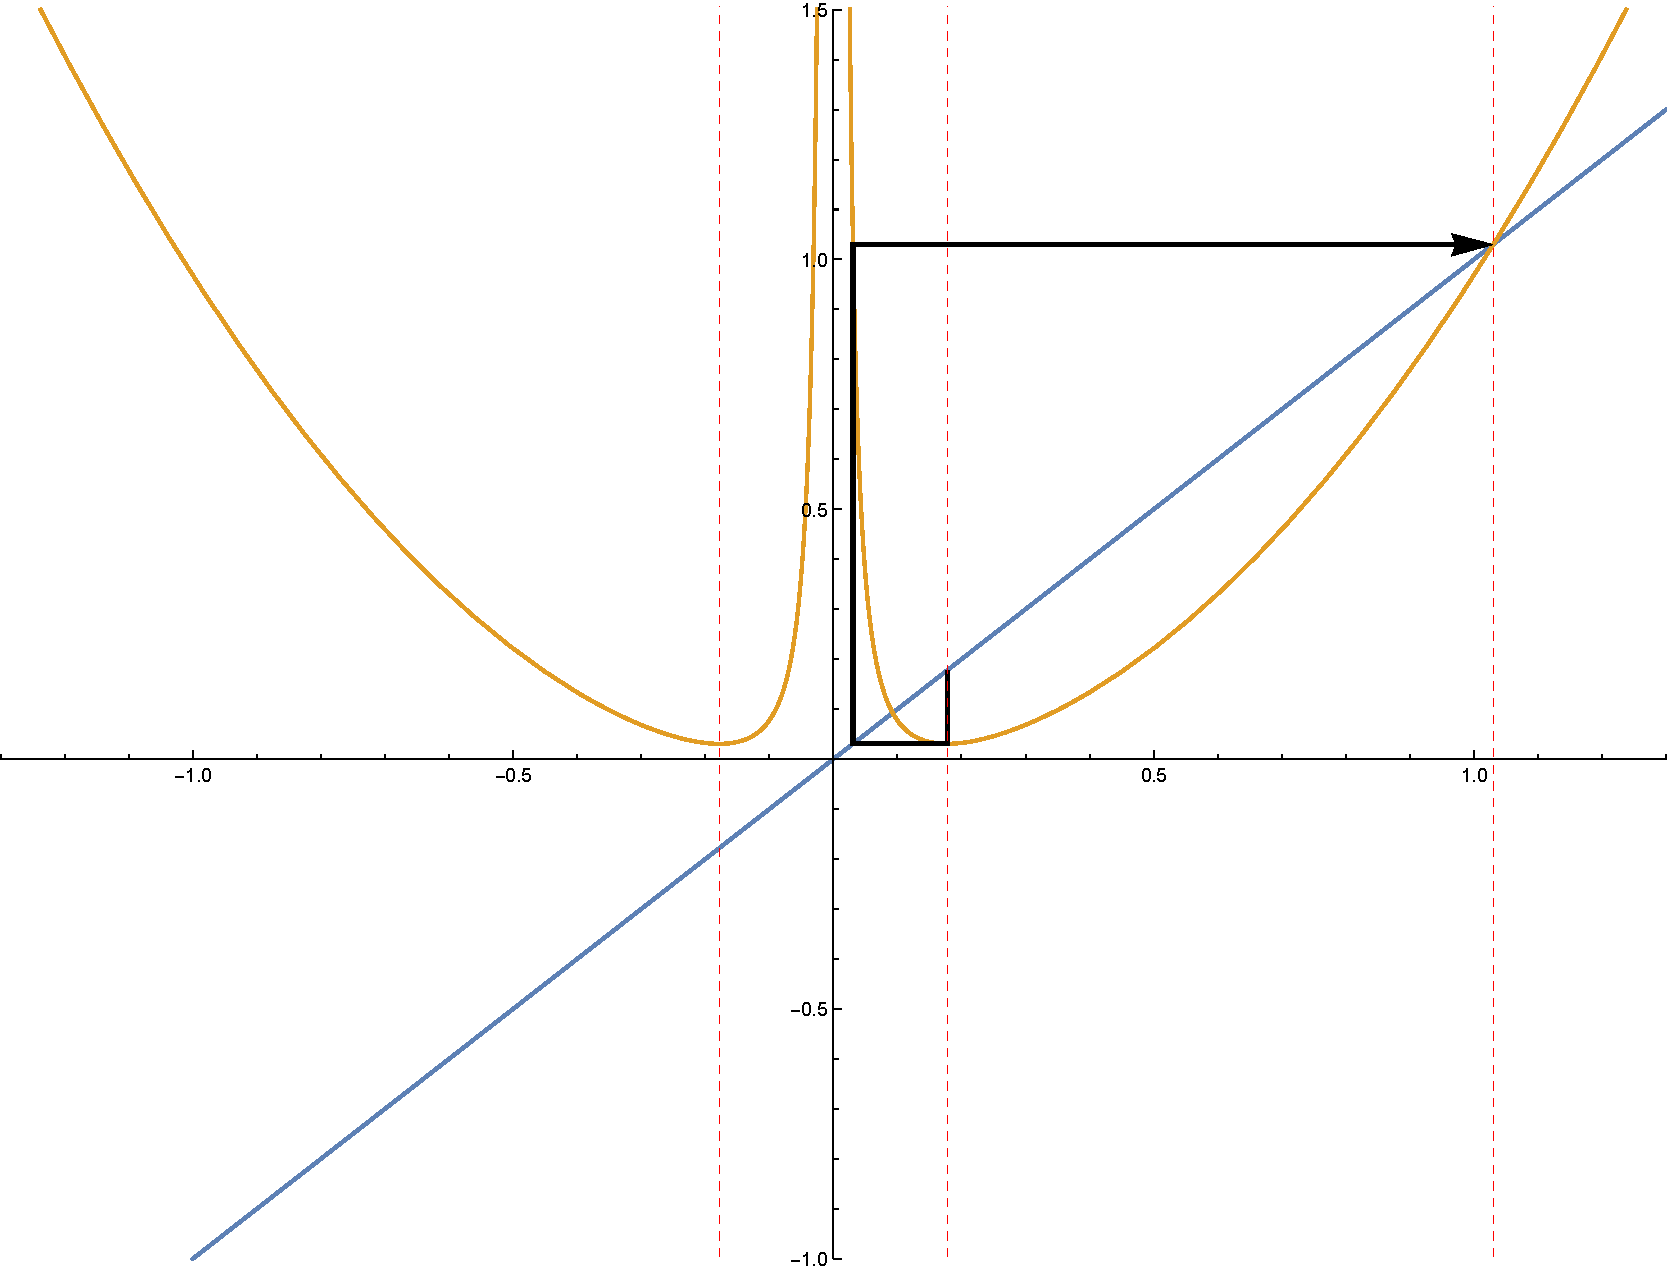
\includegraphics[width=\textwidth]{./img/plot-003255}
				\caption{$c \approx -.03255 \approx h_2^{CLP_c}$}
		\end{subfigure}

		\begin{subfigure}[b]{0.3\textwidth}
				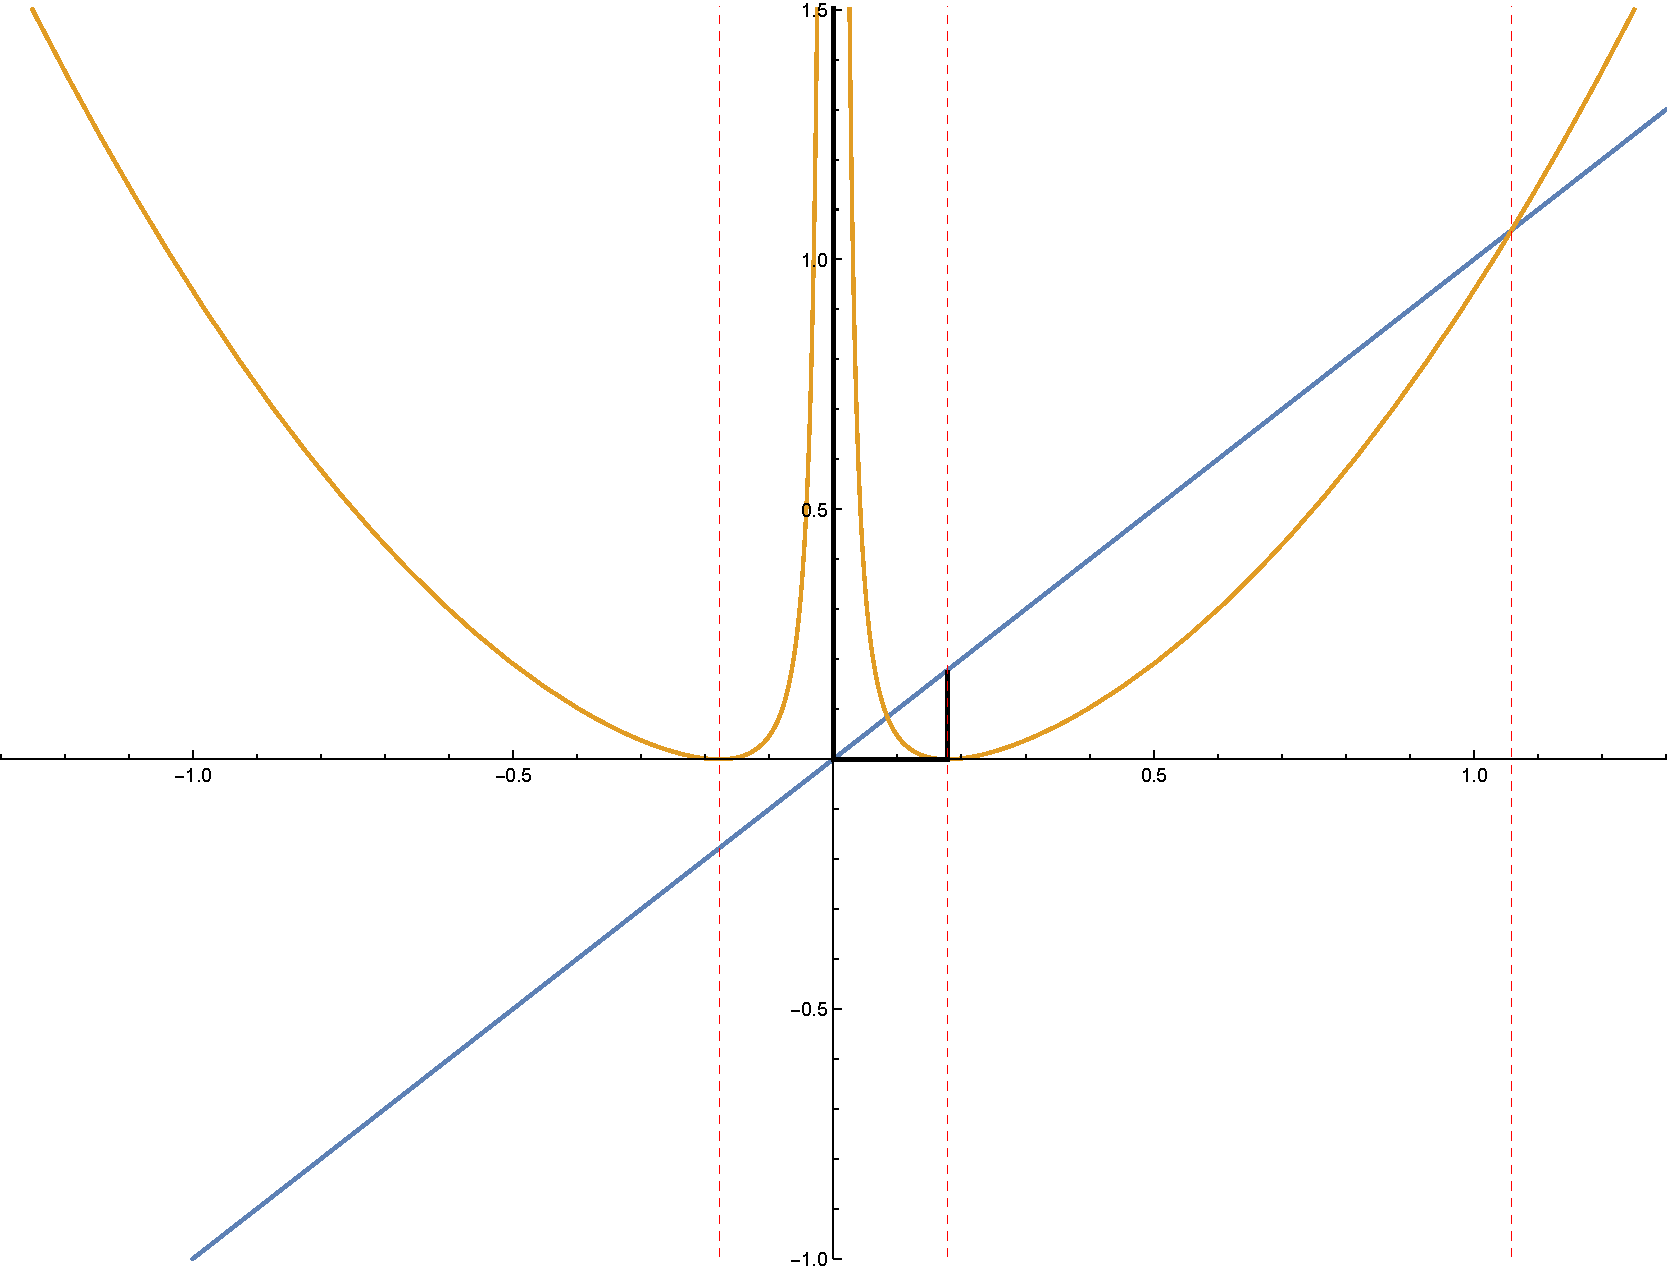
\includegraphics[width=\textwidth]{./img/plot-006355}
				\caption{$c \approx -.06335 \approx z_1^{C0}$}
		\end{subfigure}
		\begin{subfigure}[b]{0.3\textwidth}
				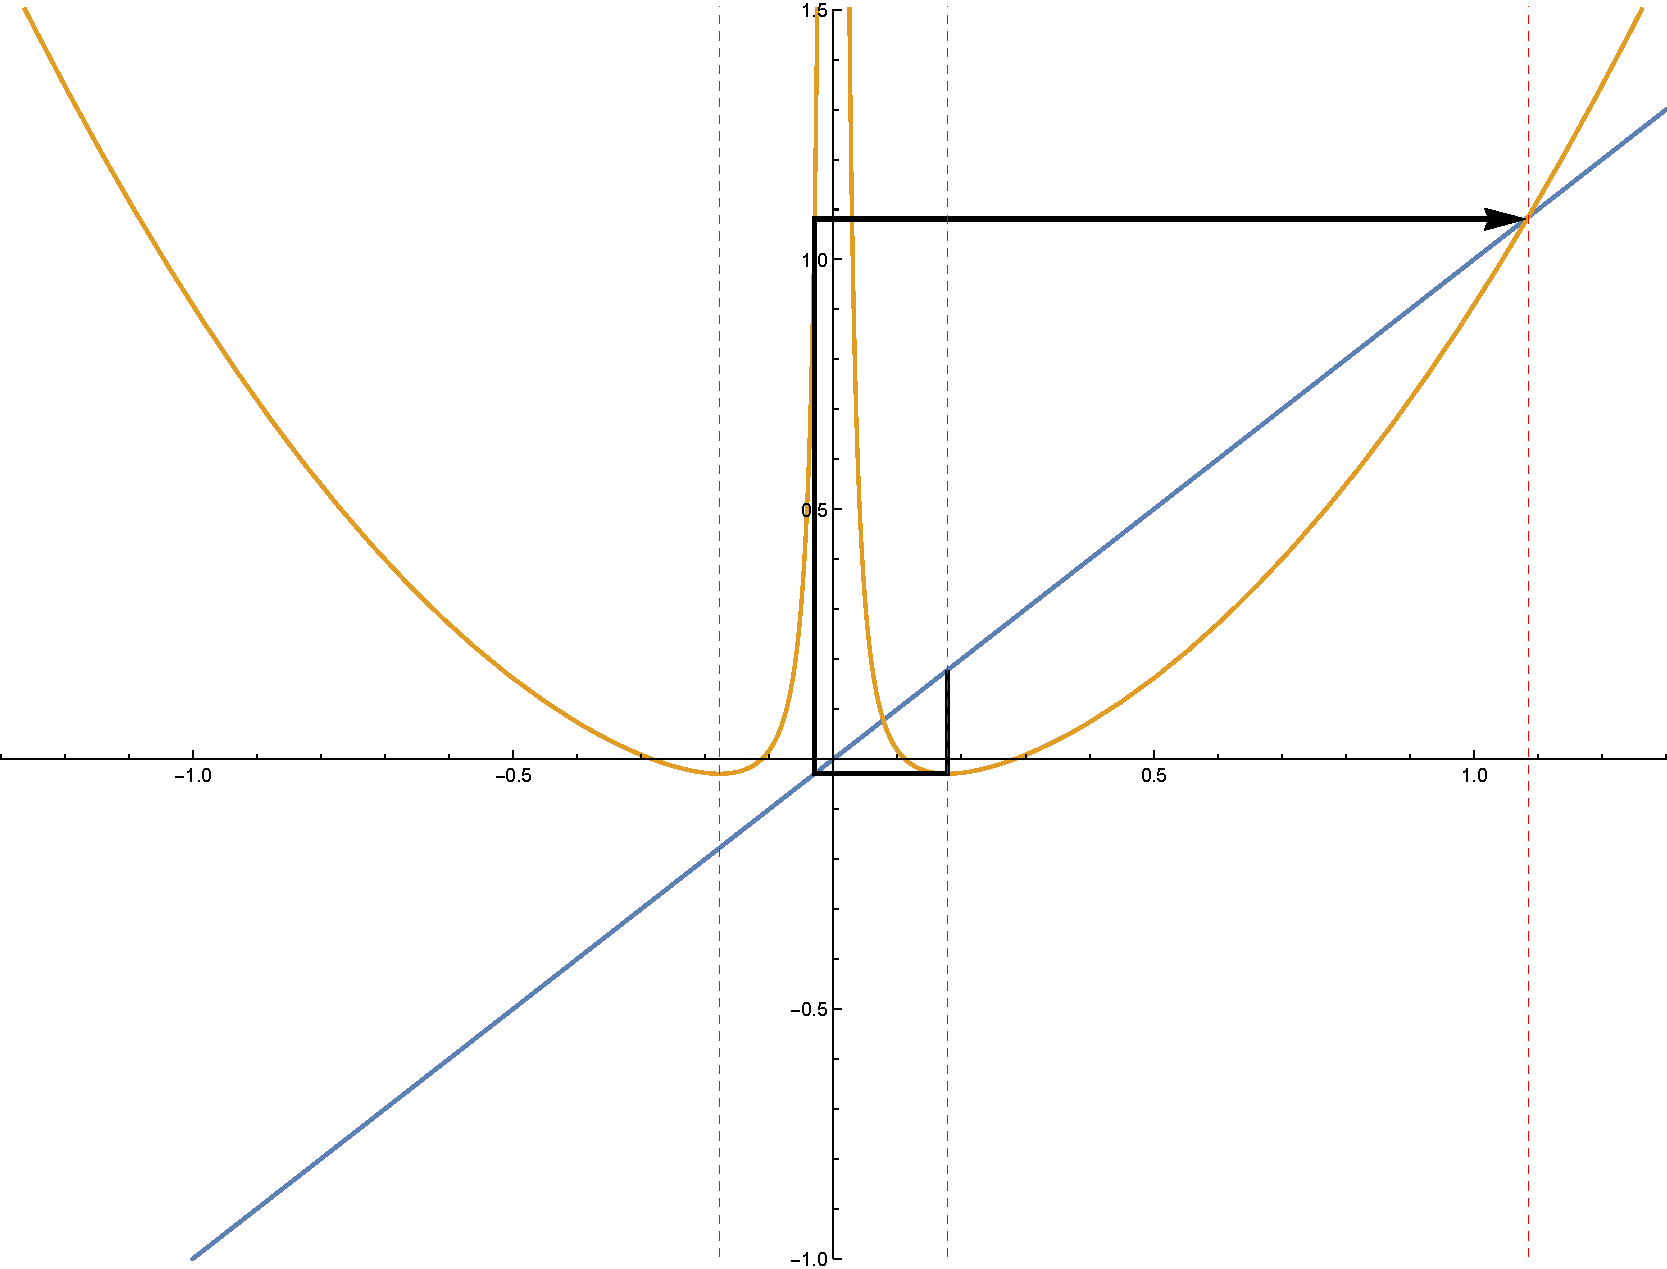
\includegraphics[width=\textwidth]{./img/plot-009245}
				\caption{$c \approx -.09245 \approx h_2^{CrP_c}$}
		\end{subfigure}
		\begin{subfigure}[b]{0.3\textwidth}
				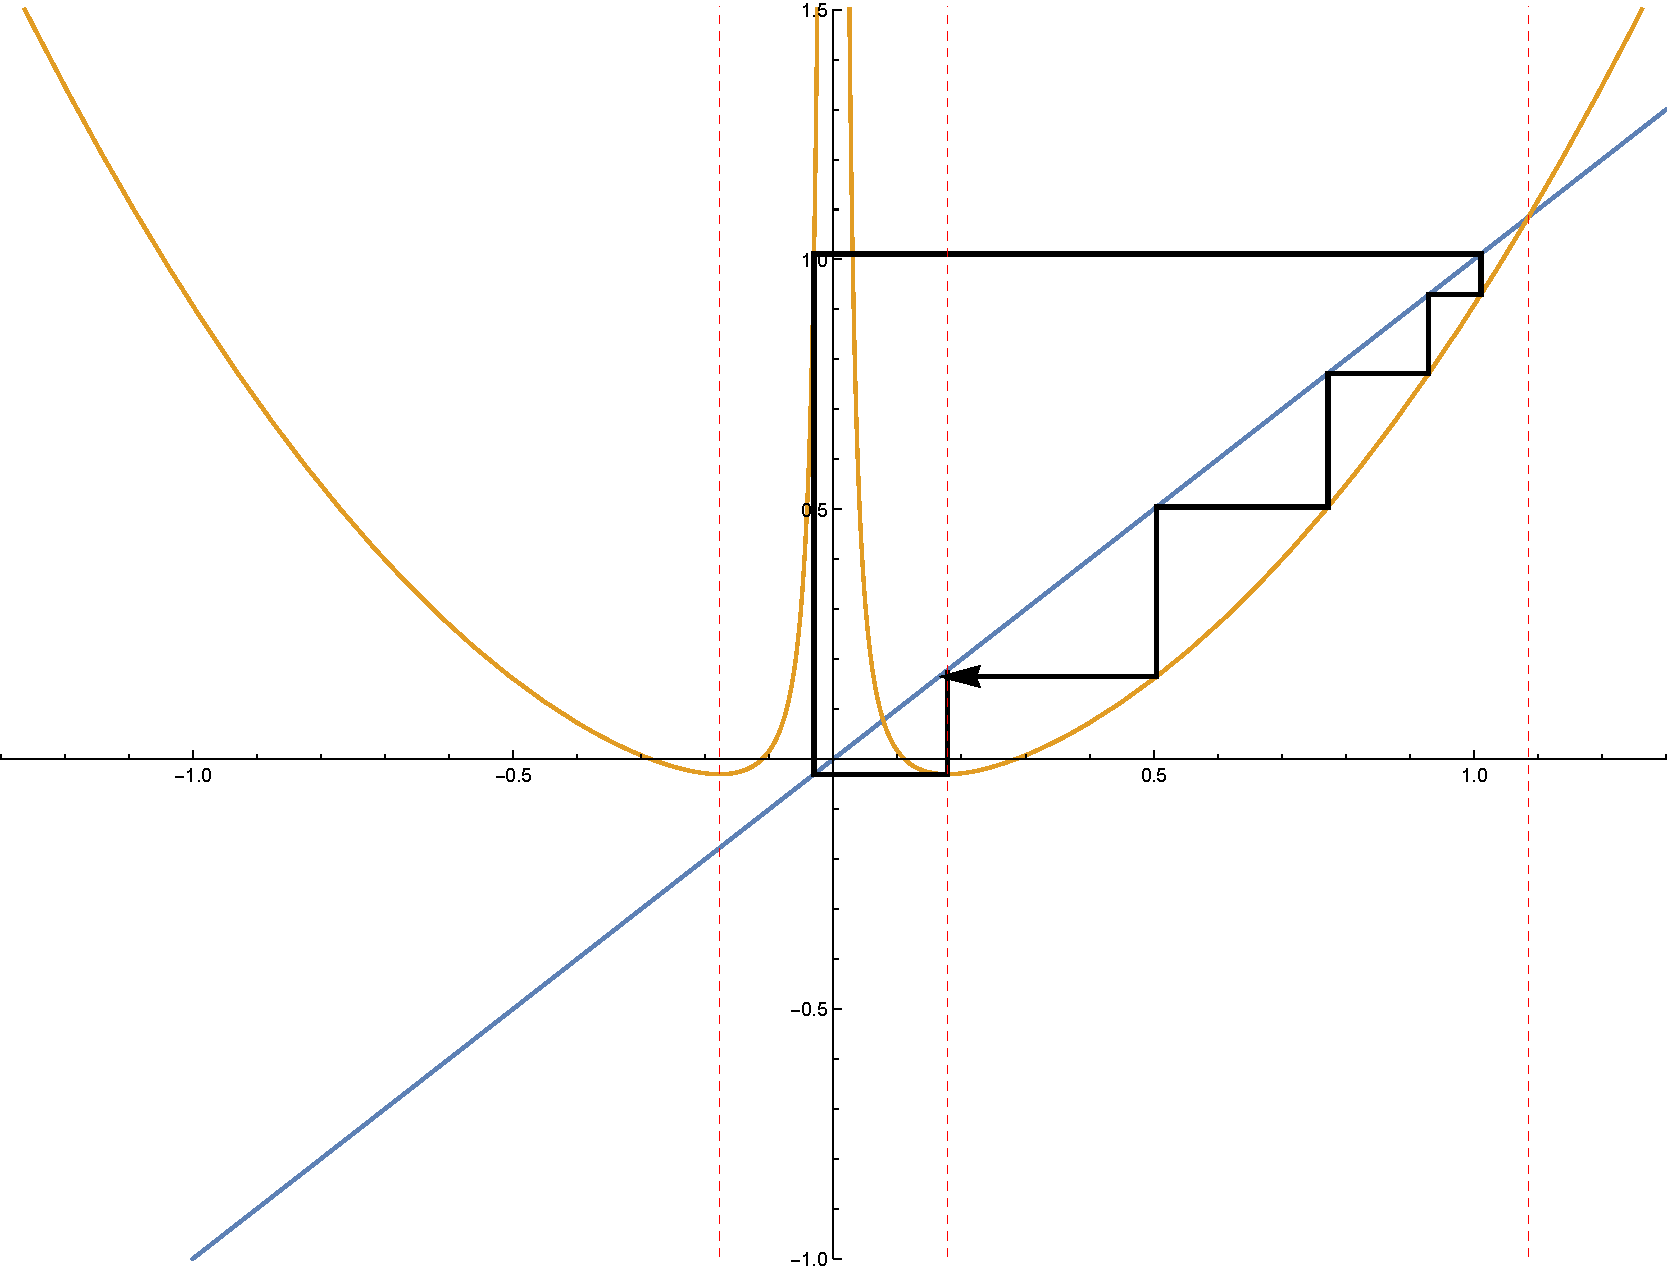
\includegraphics[width=\textwidth]{./img/plot-009335}
				\caption{$c \approx -.09335 \approx p_6^{CrFFFFC}$}
		\end{subfigure}

		\begin{subfigure}[b]{0.3\textwidth}
				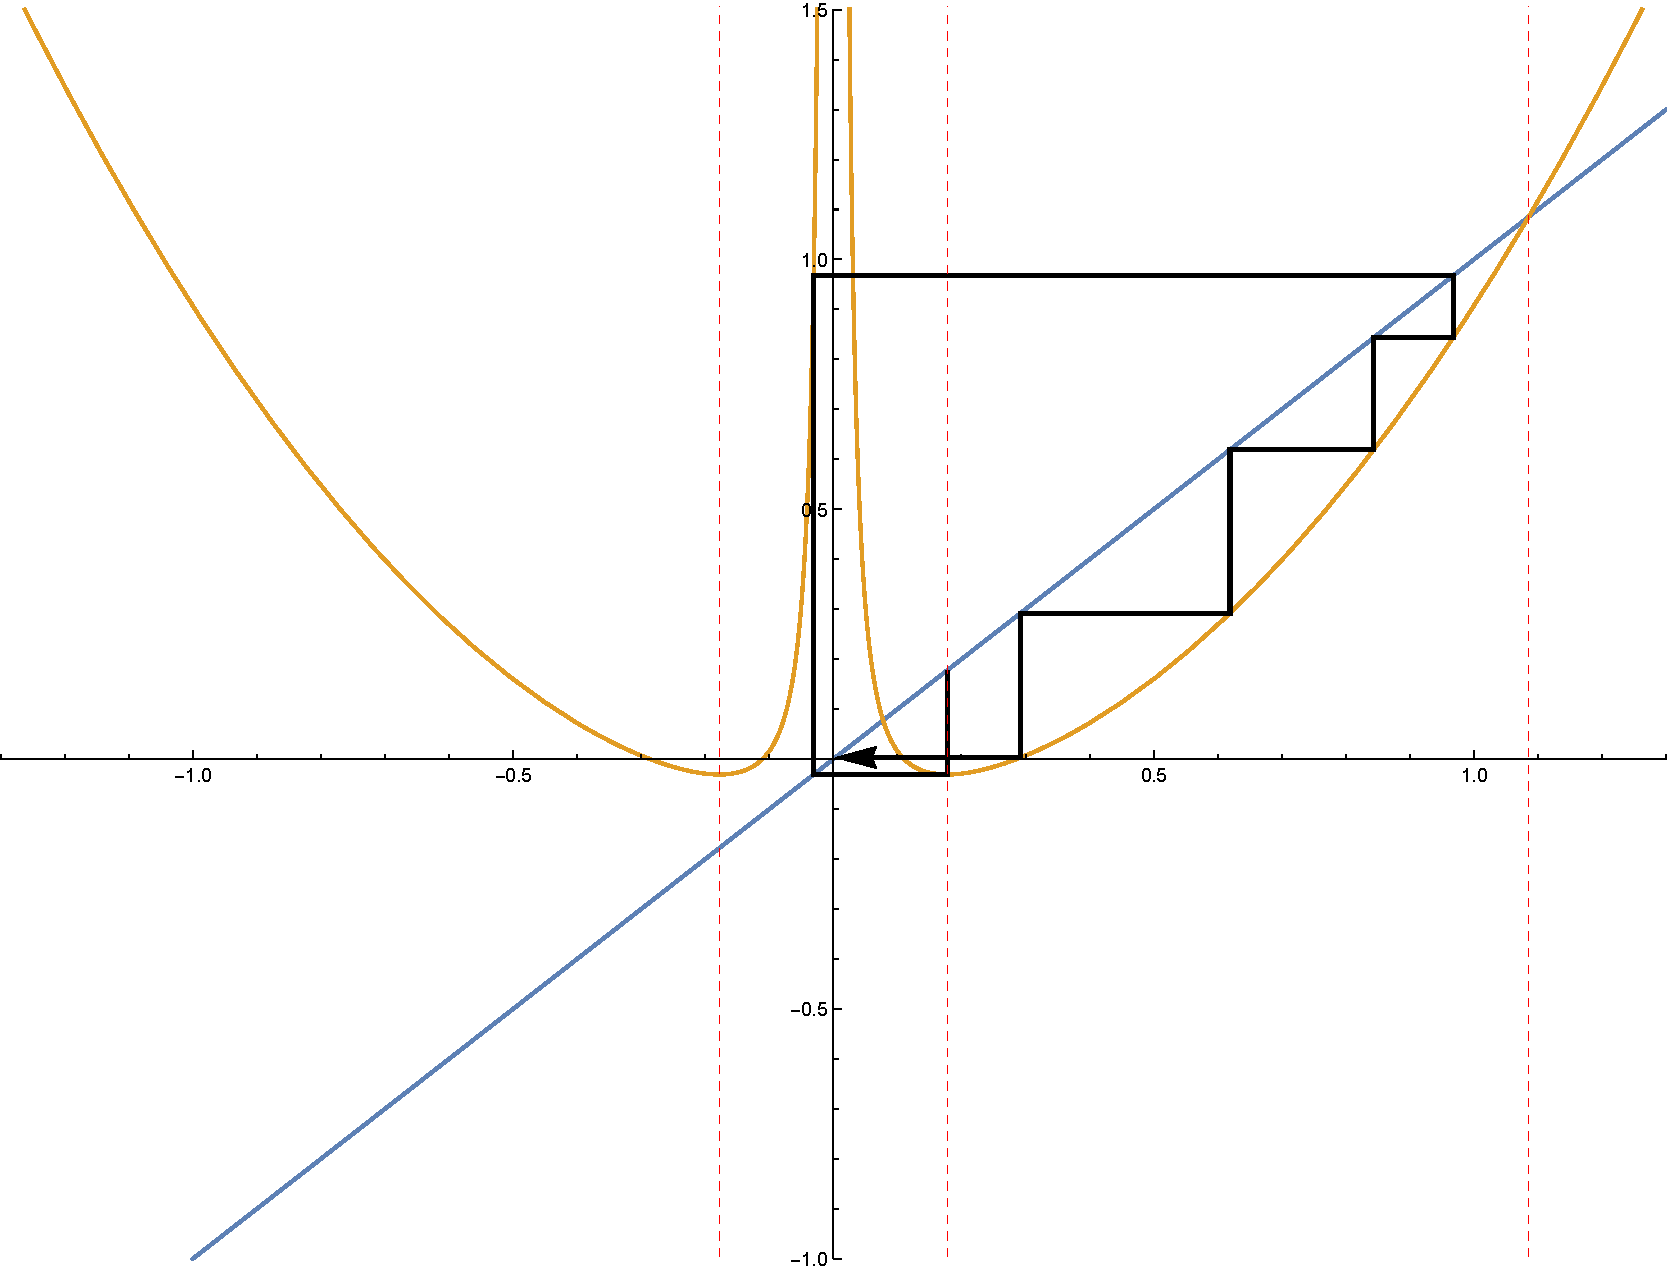
\includegraphics[width=\textwidth]{./img/plot-009395}
				\caption{$c \approx - .09395 \approx z_6^{CrFFFF0}$}
		\end{subfigure}
		\begin{subfigure}[b]{0.3\textwidth}
				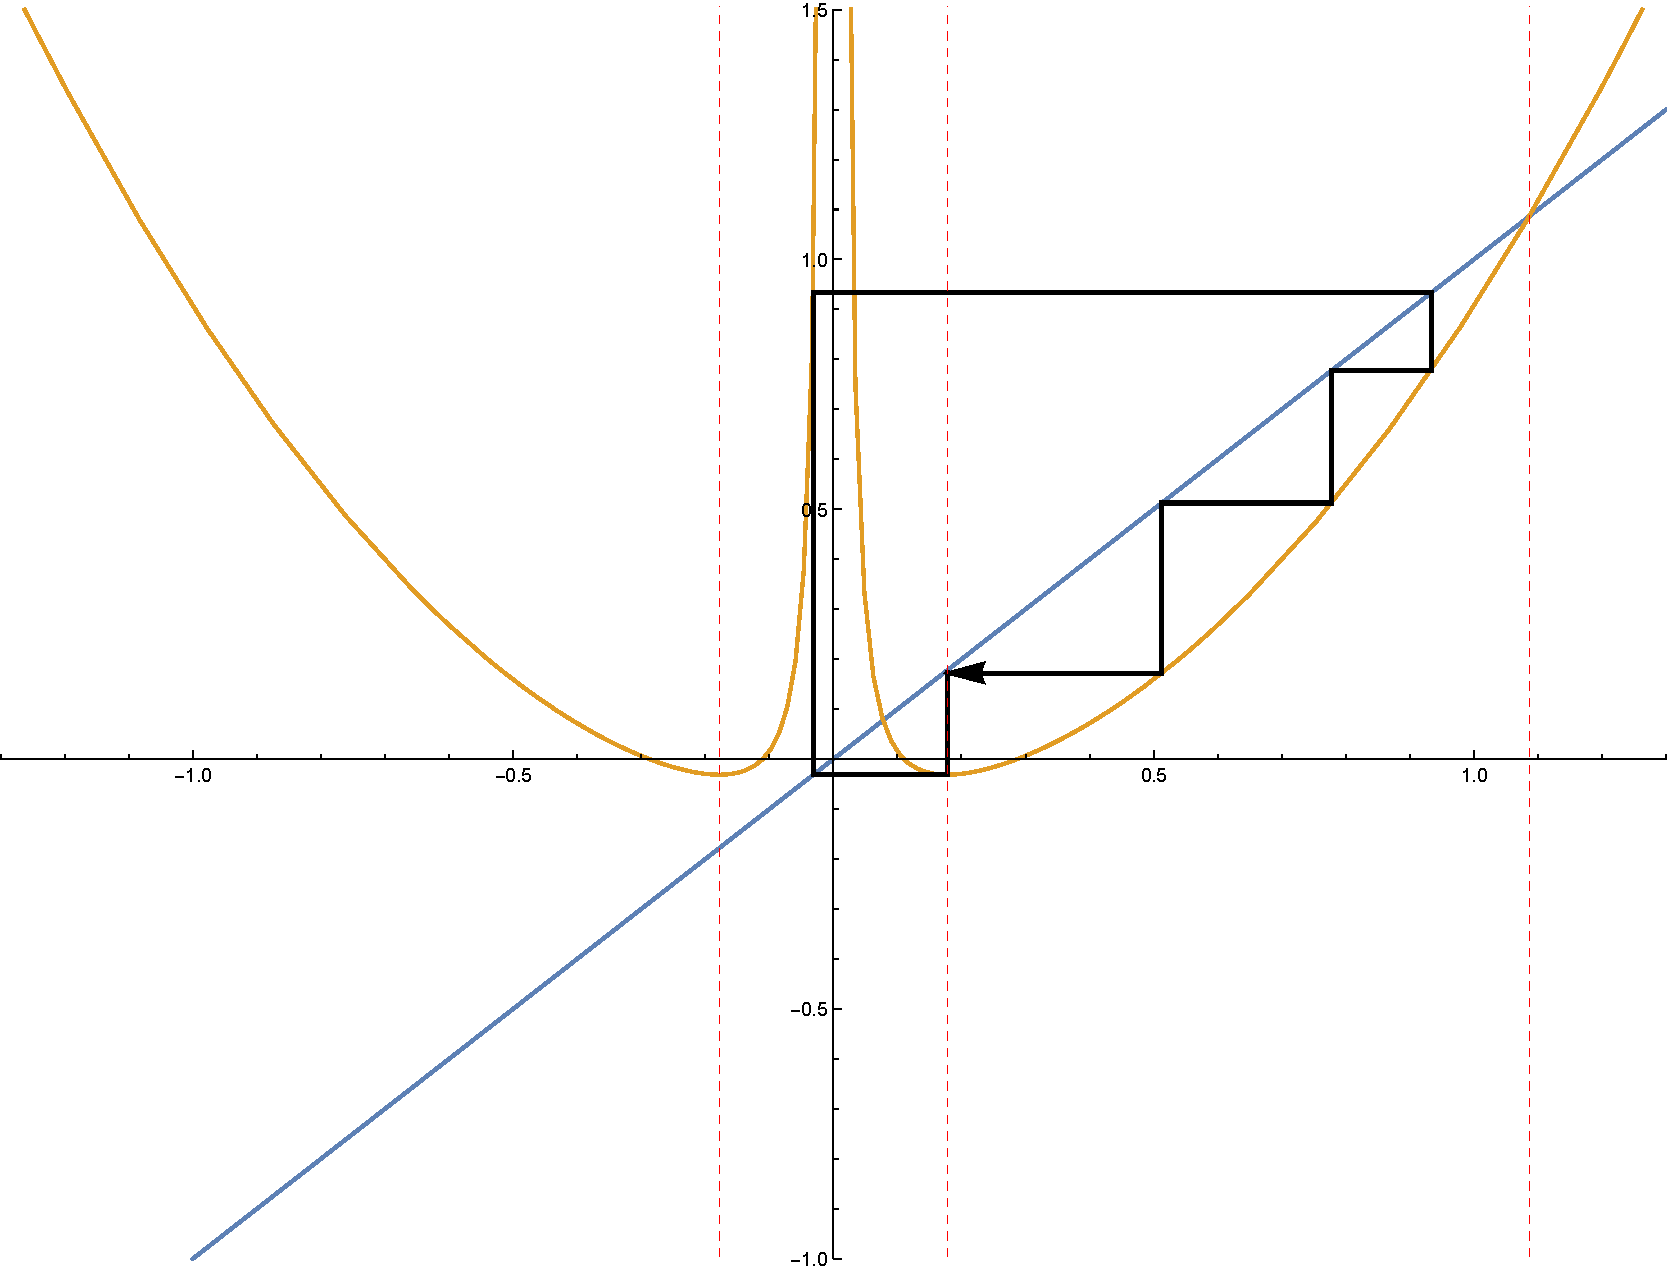
\includegraphics[width=\textwidth]{./img/plot-009445}
				\caption{$c \approx -.09445 \approx p_5^{CrFFFC}$}
		\end{subfigure}
		\begin{subfigure}[b]{0.3\textwidth}
				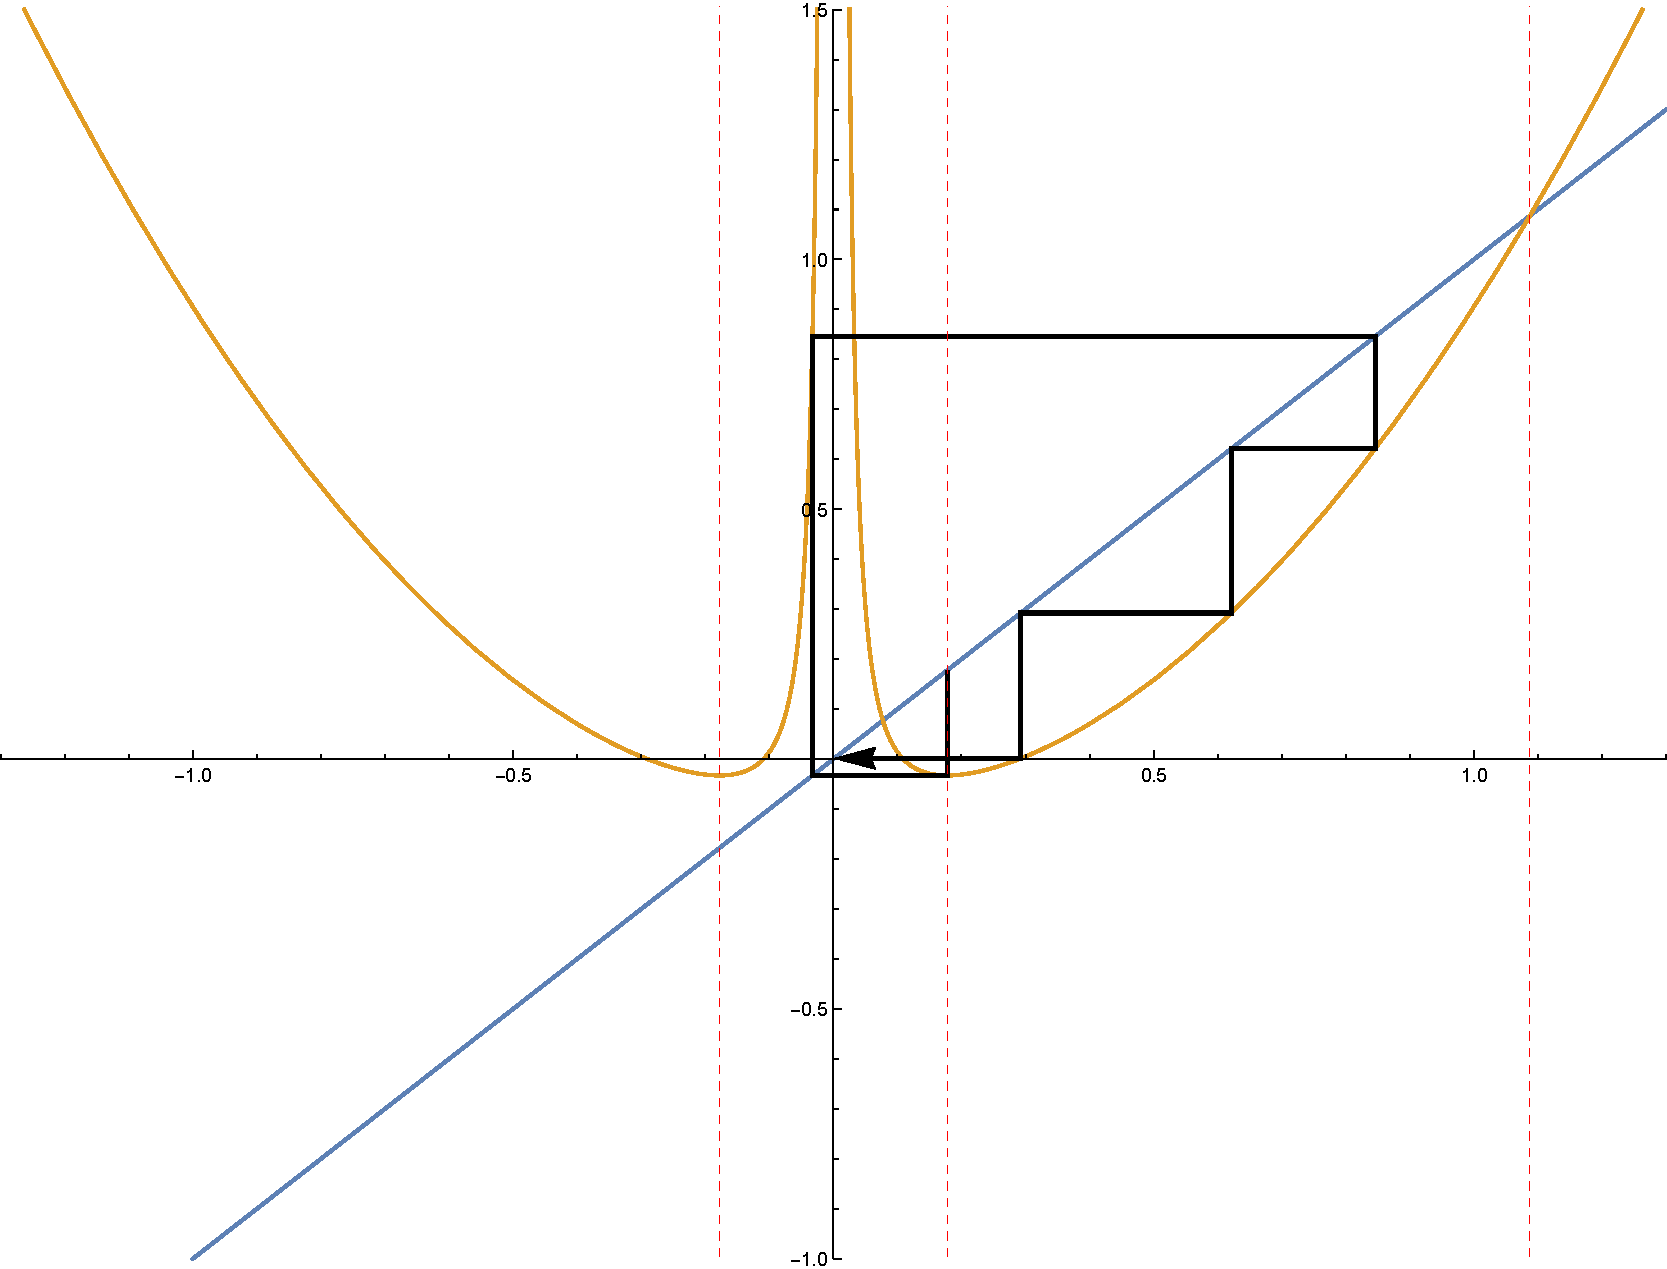
\includegraphics[width=\textwidth]{./img/plot-009585}
				\caption{$c \approx -.09585 \approx z_5^{CrFFF0}$}
		\end{subfigure}

		\begin{subfigure}[b]{0.3\textwidth}
				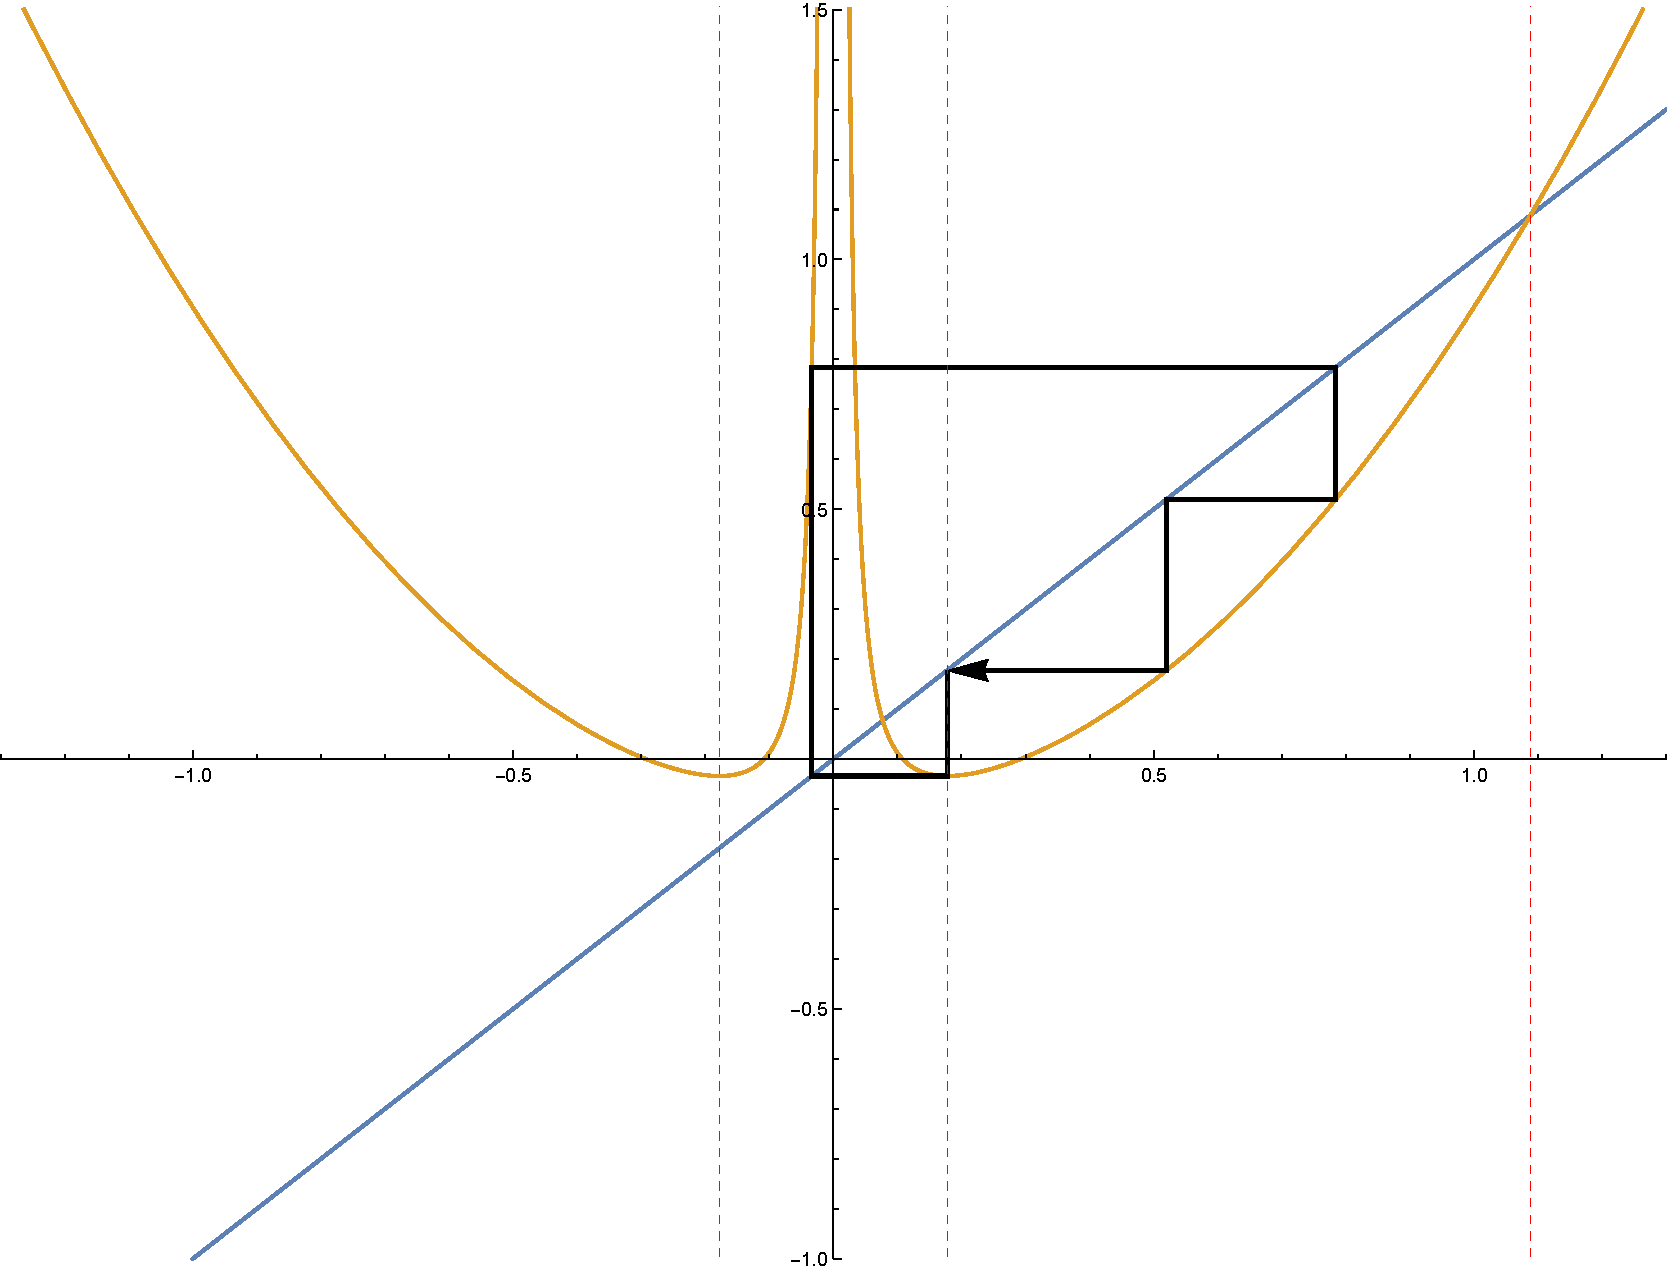
\includegraphics[width=\textwidth]{./img/plot-009695}
				\caption{$c \approx -.09695 \approx p_4^{CrFFC}$}
		\end{subfigure}
		\begin{subfigure}[b]{0.3\textwidth}
				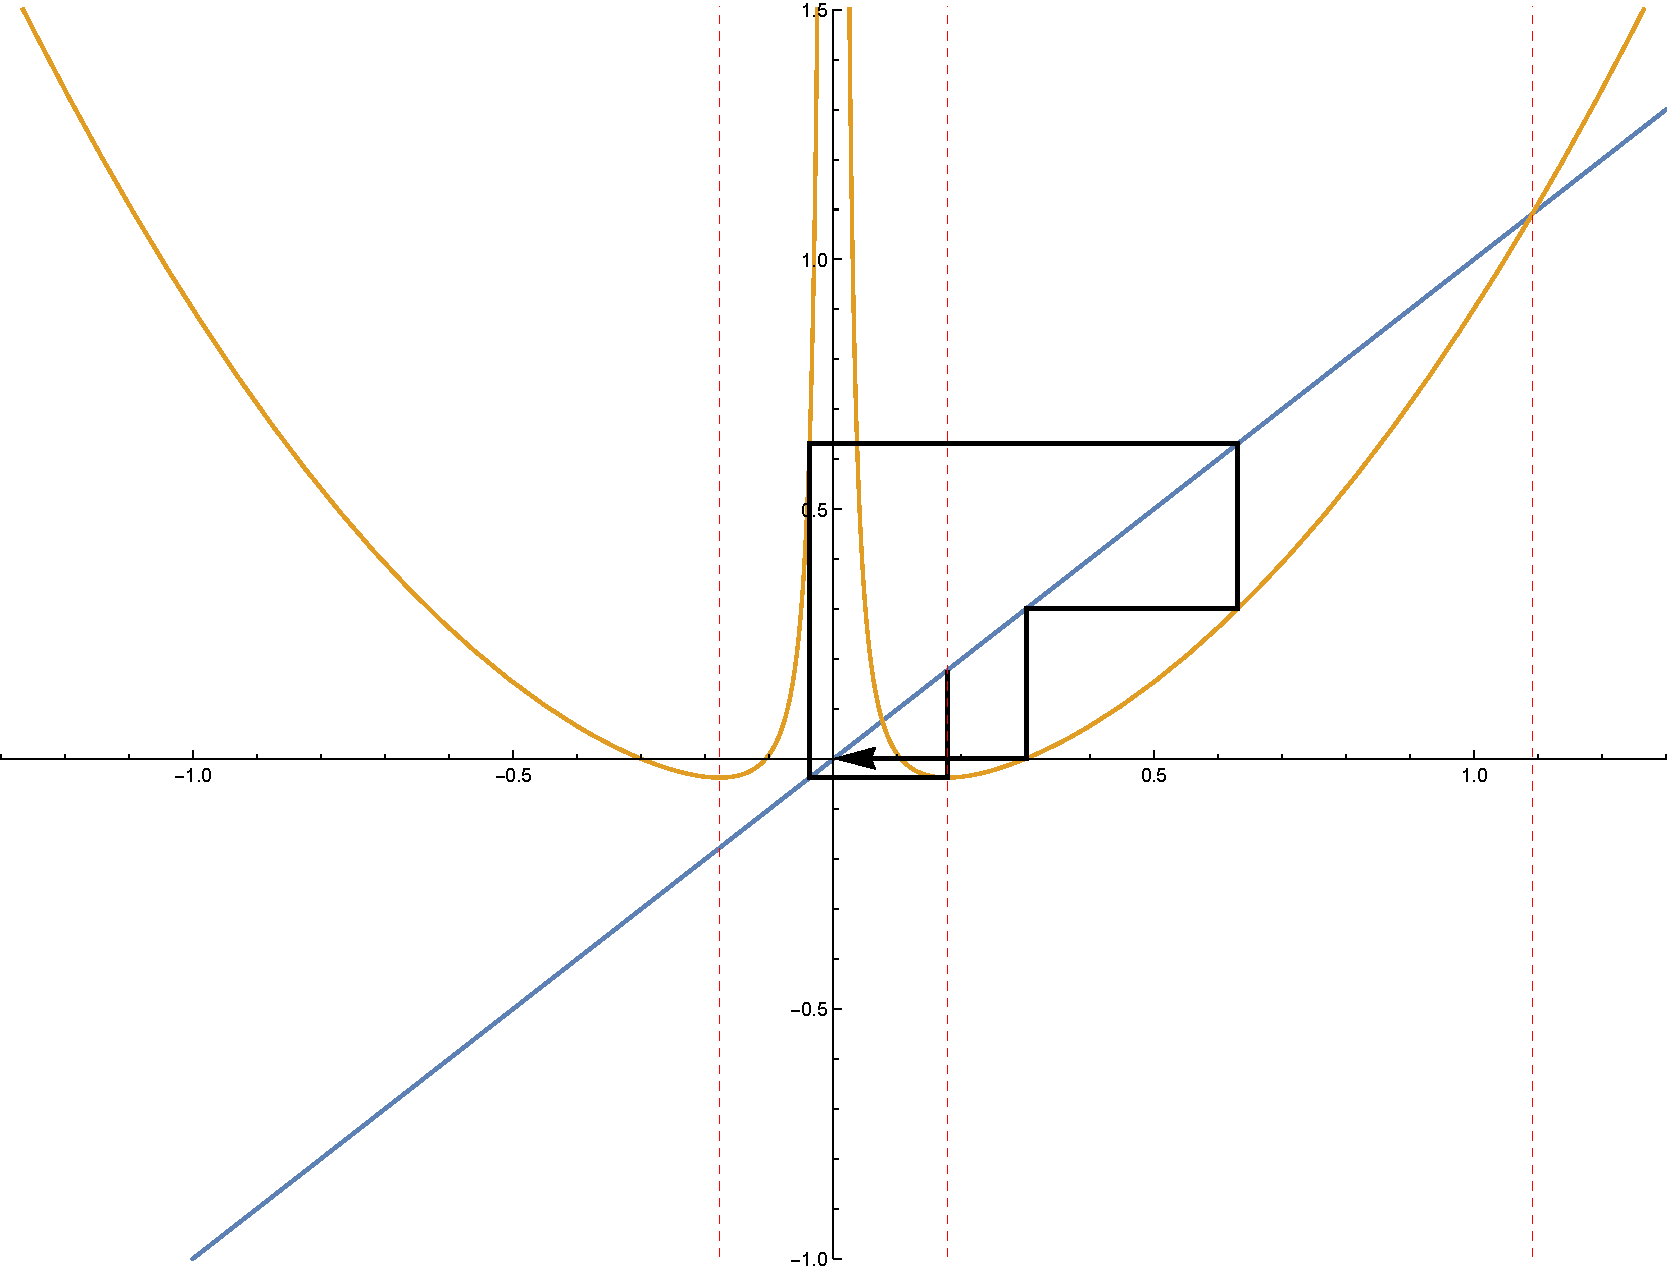
\includegraphics[width=\textwidth]{./img/plot-010025}
				\caption{$c \approx -.10025 \approx z_4^{CrFF0}$}
		\end{subfigure}
		\begin{subfigure}[b]{0.3\textwidth}
				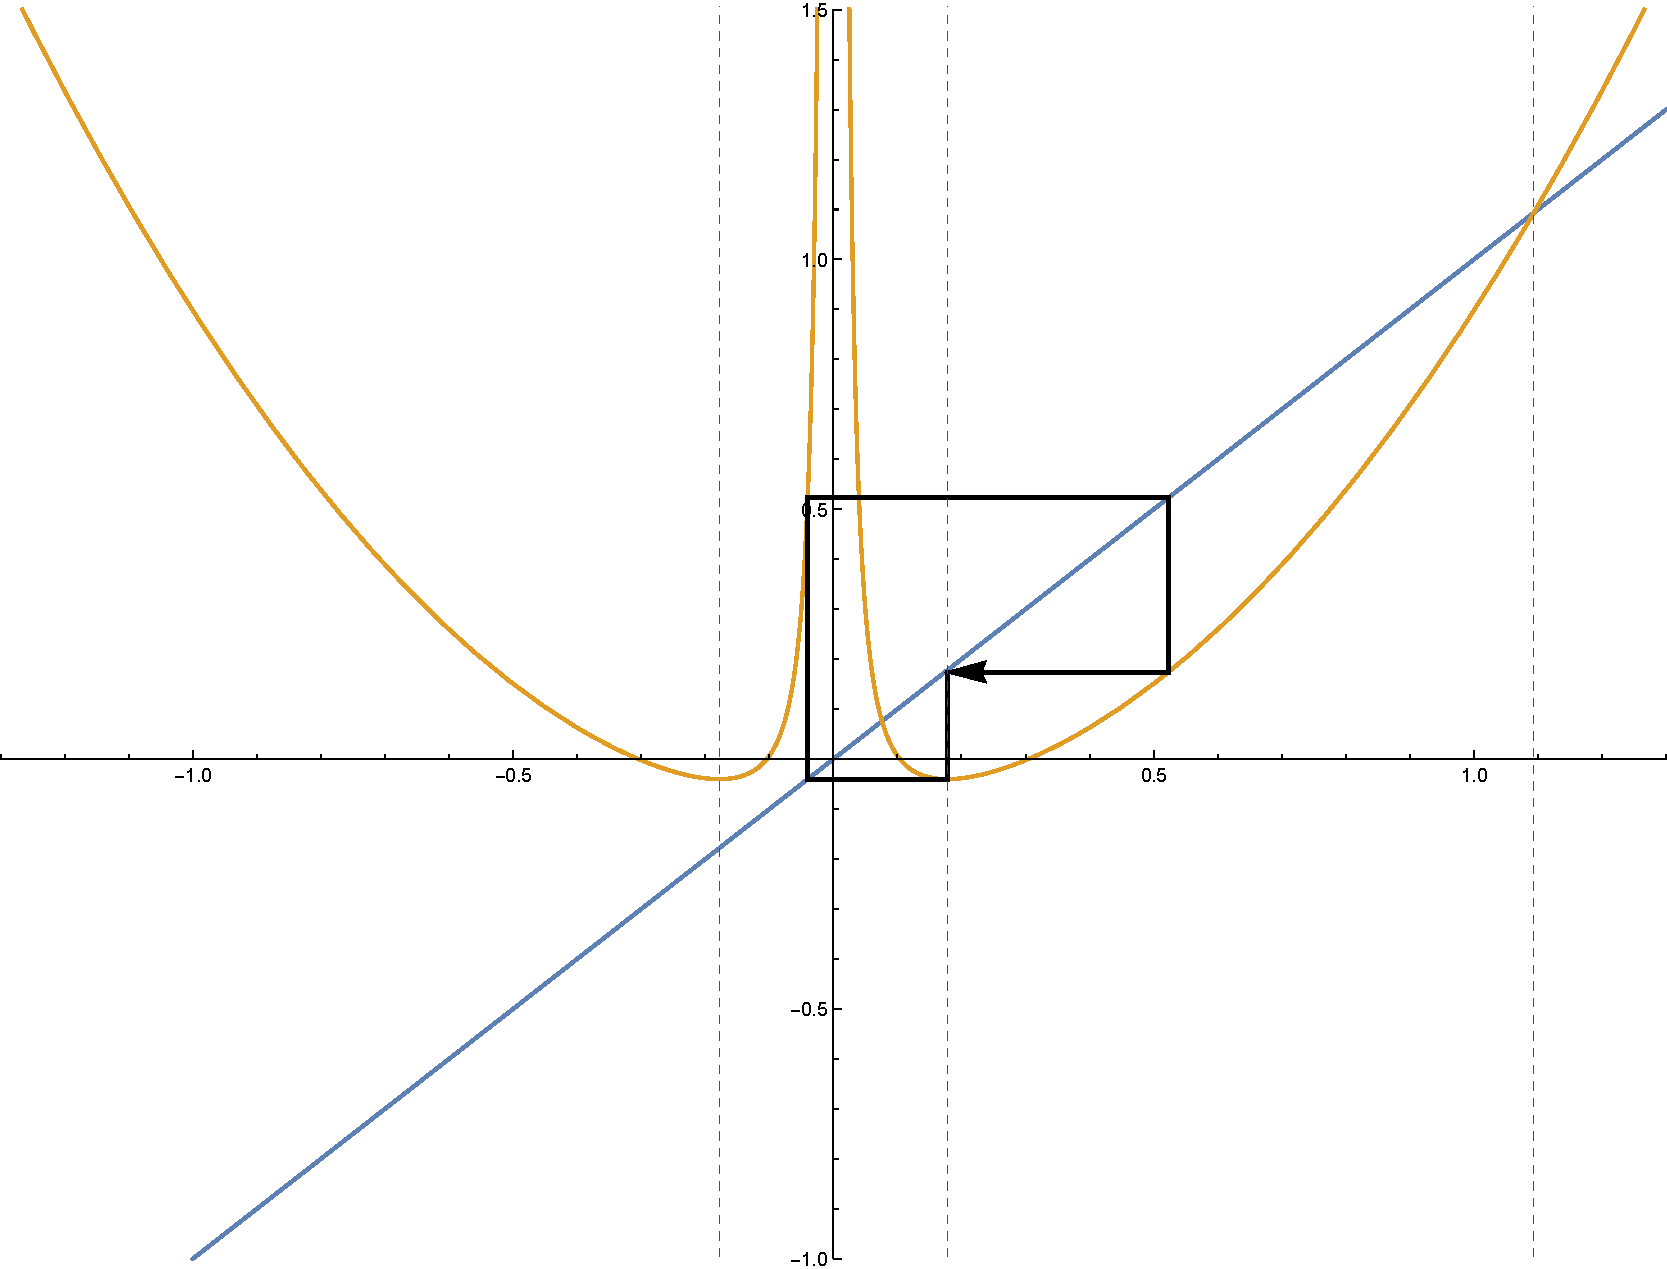
\includegraphics[width=\textwidth]{./img/plot-010325}
				\caption{$c \approx - .10325 \approx p_3^{CrFC}$}
		\end{subfigure}

		\begin{subfigure}[b]{0.3\textwidth}
				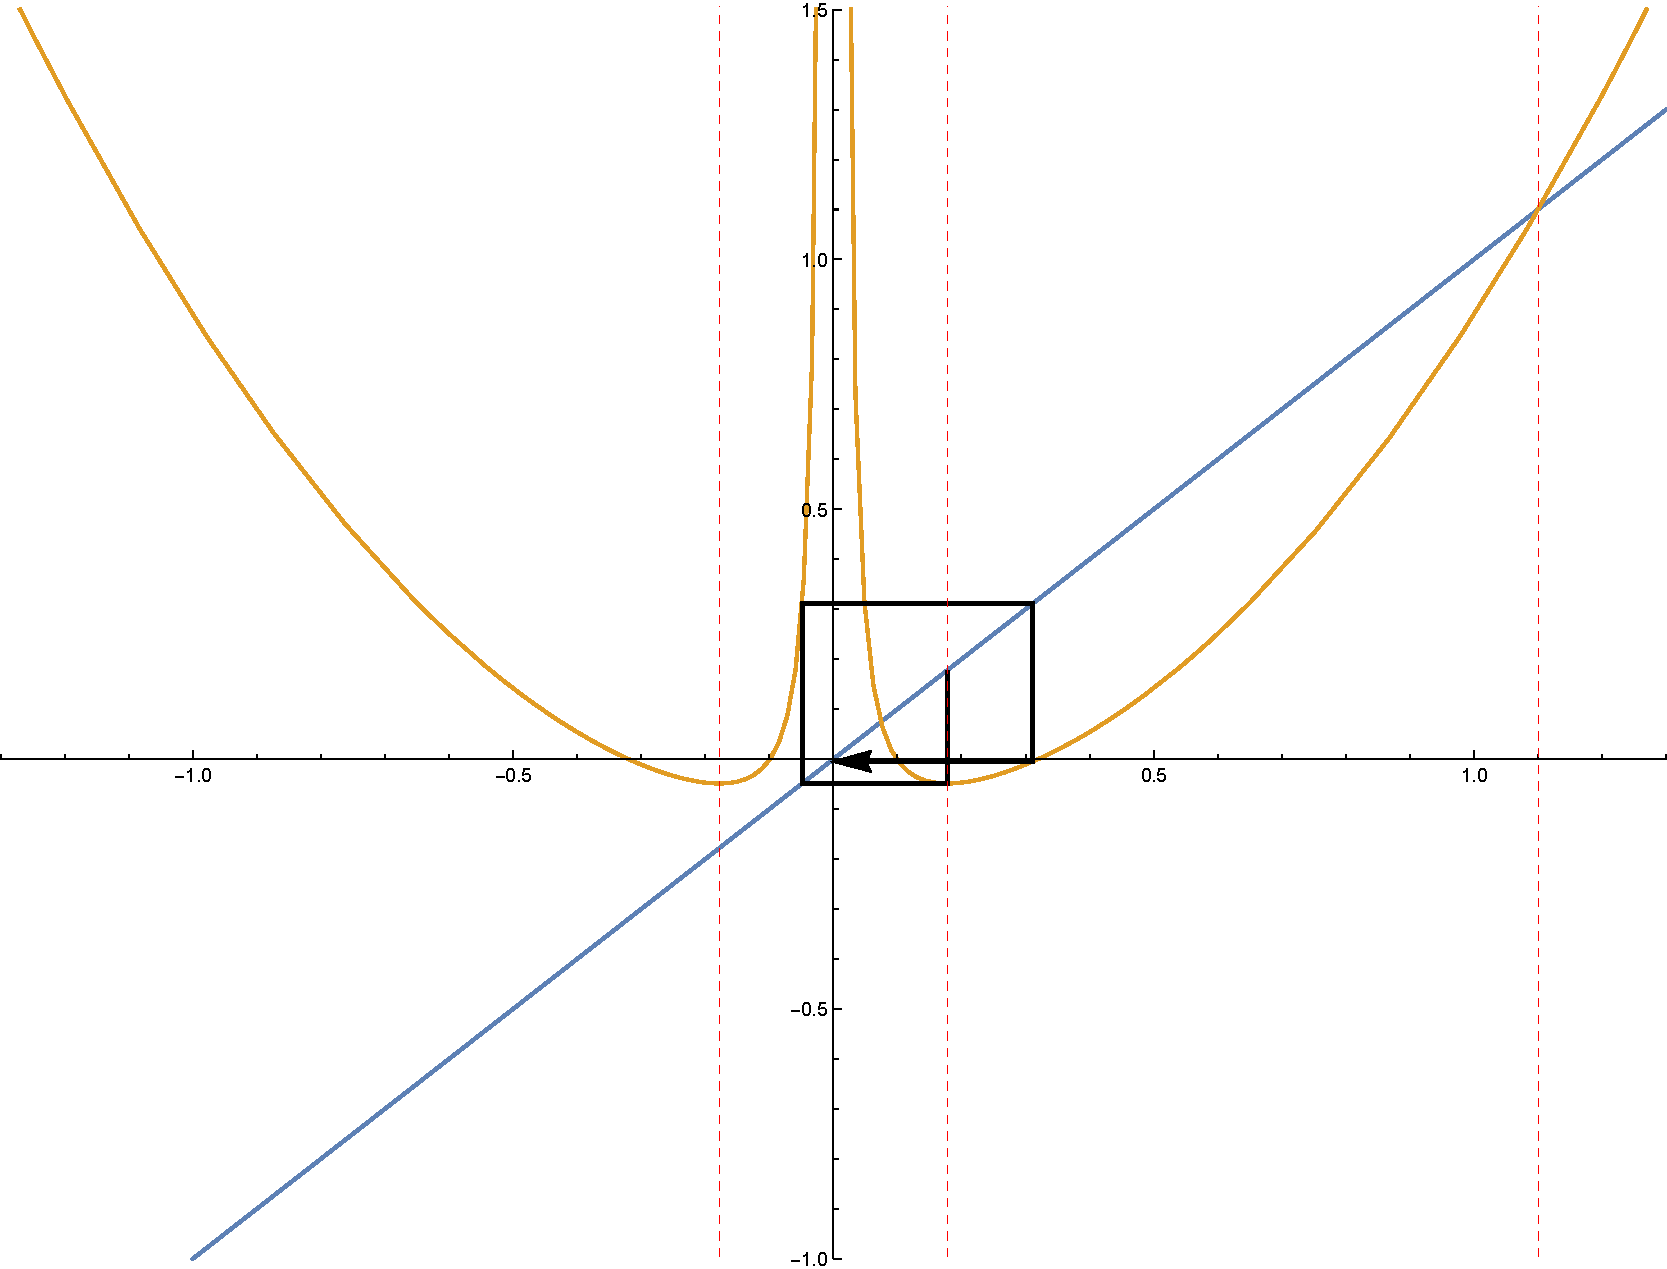
\includegraphics[width=\textwidth]{./img/plot-0112}
				\caption{$c \approx -.112 \approx z_3^{CrF0}$}
		\end{subfigure}
		\begin{subfigure}[b]{0.3\textwidth}
				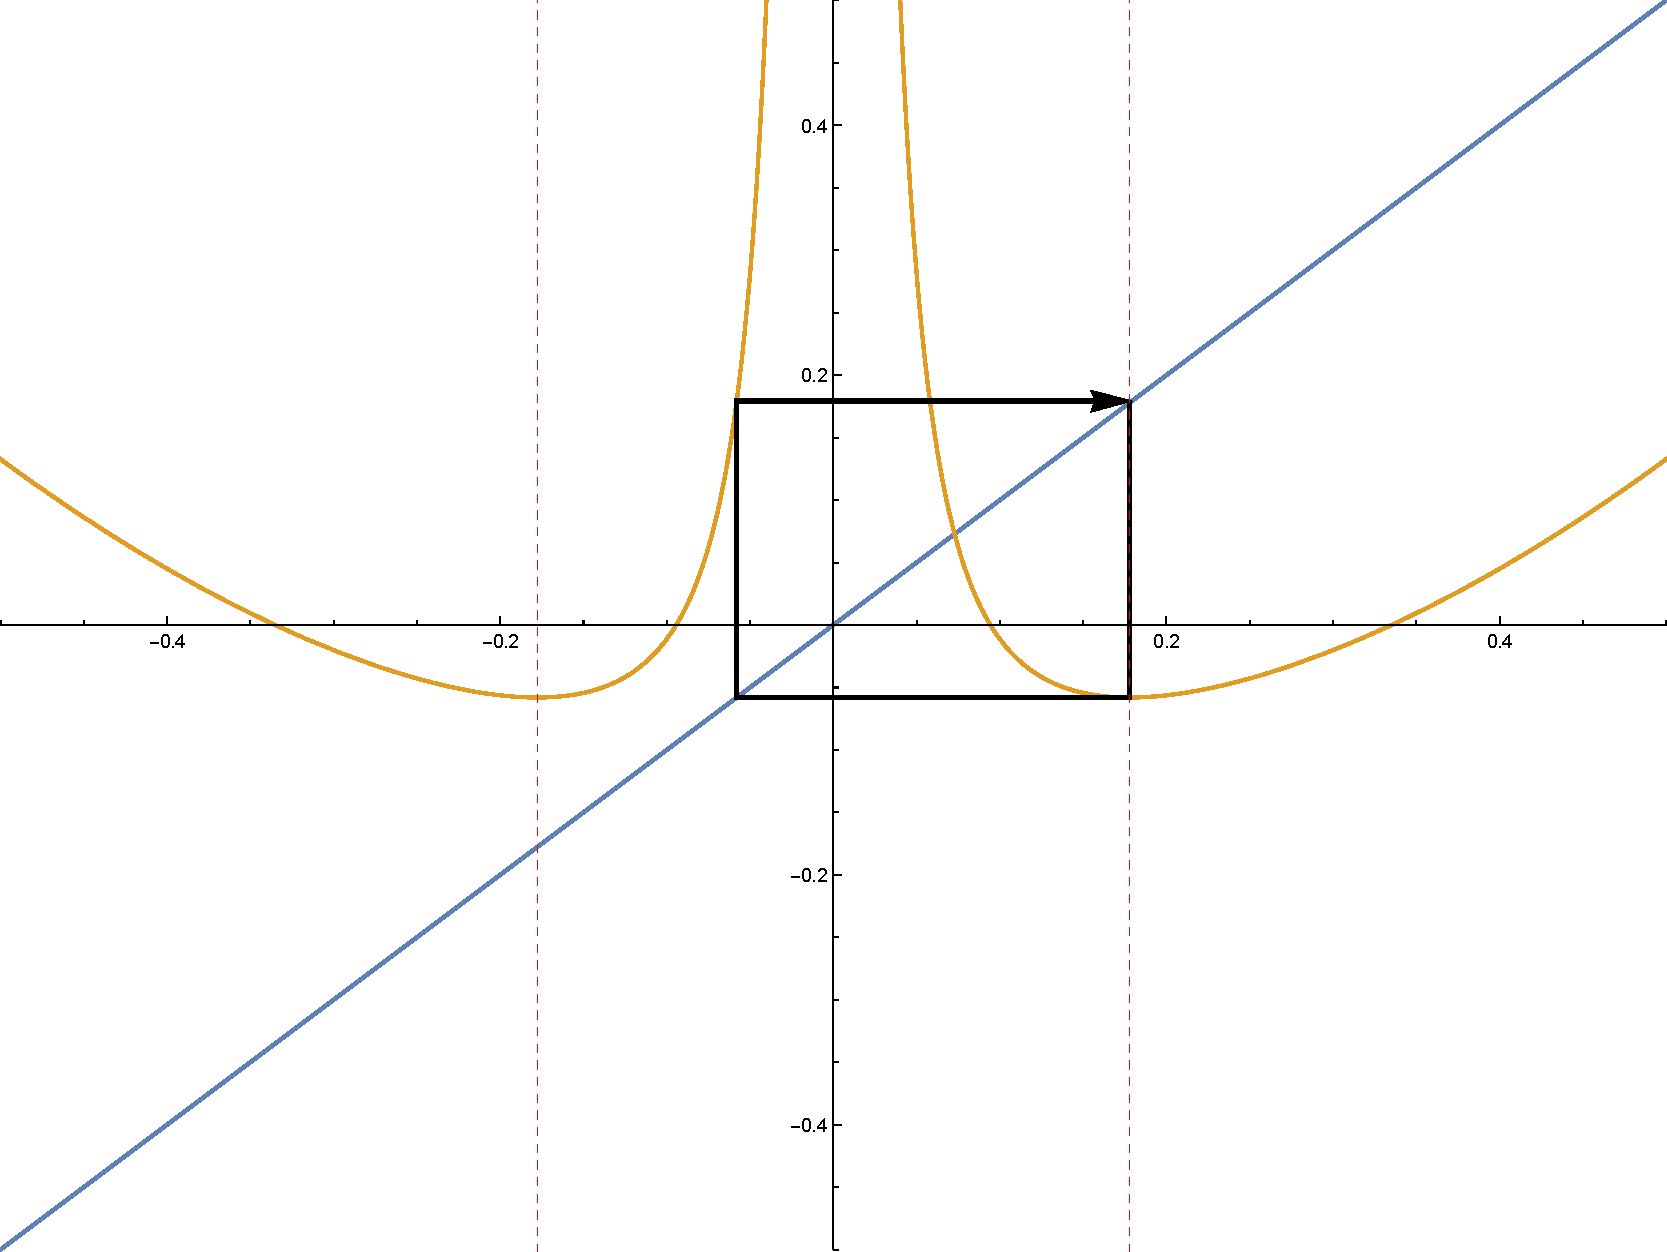
\includegraphics[width=\textwidth]{./img/plot-012125}
				\caption{$c \approx - .12125 \approx p_2^{CrC}$}
		\end{subfigure}
		\begin{subfigure}[b]{0.3\textwidth}
				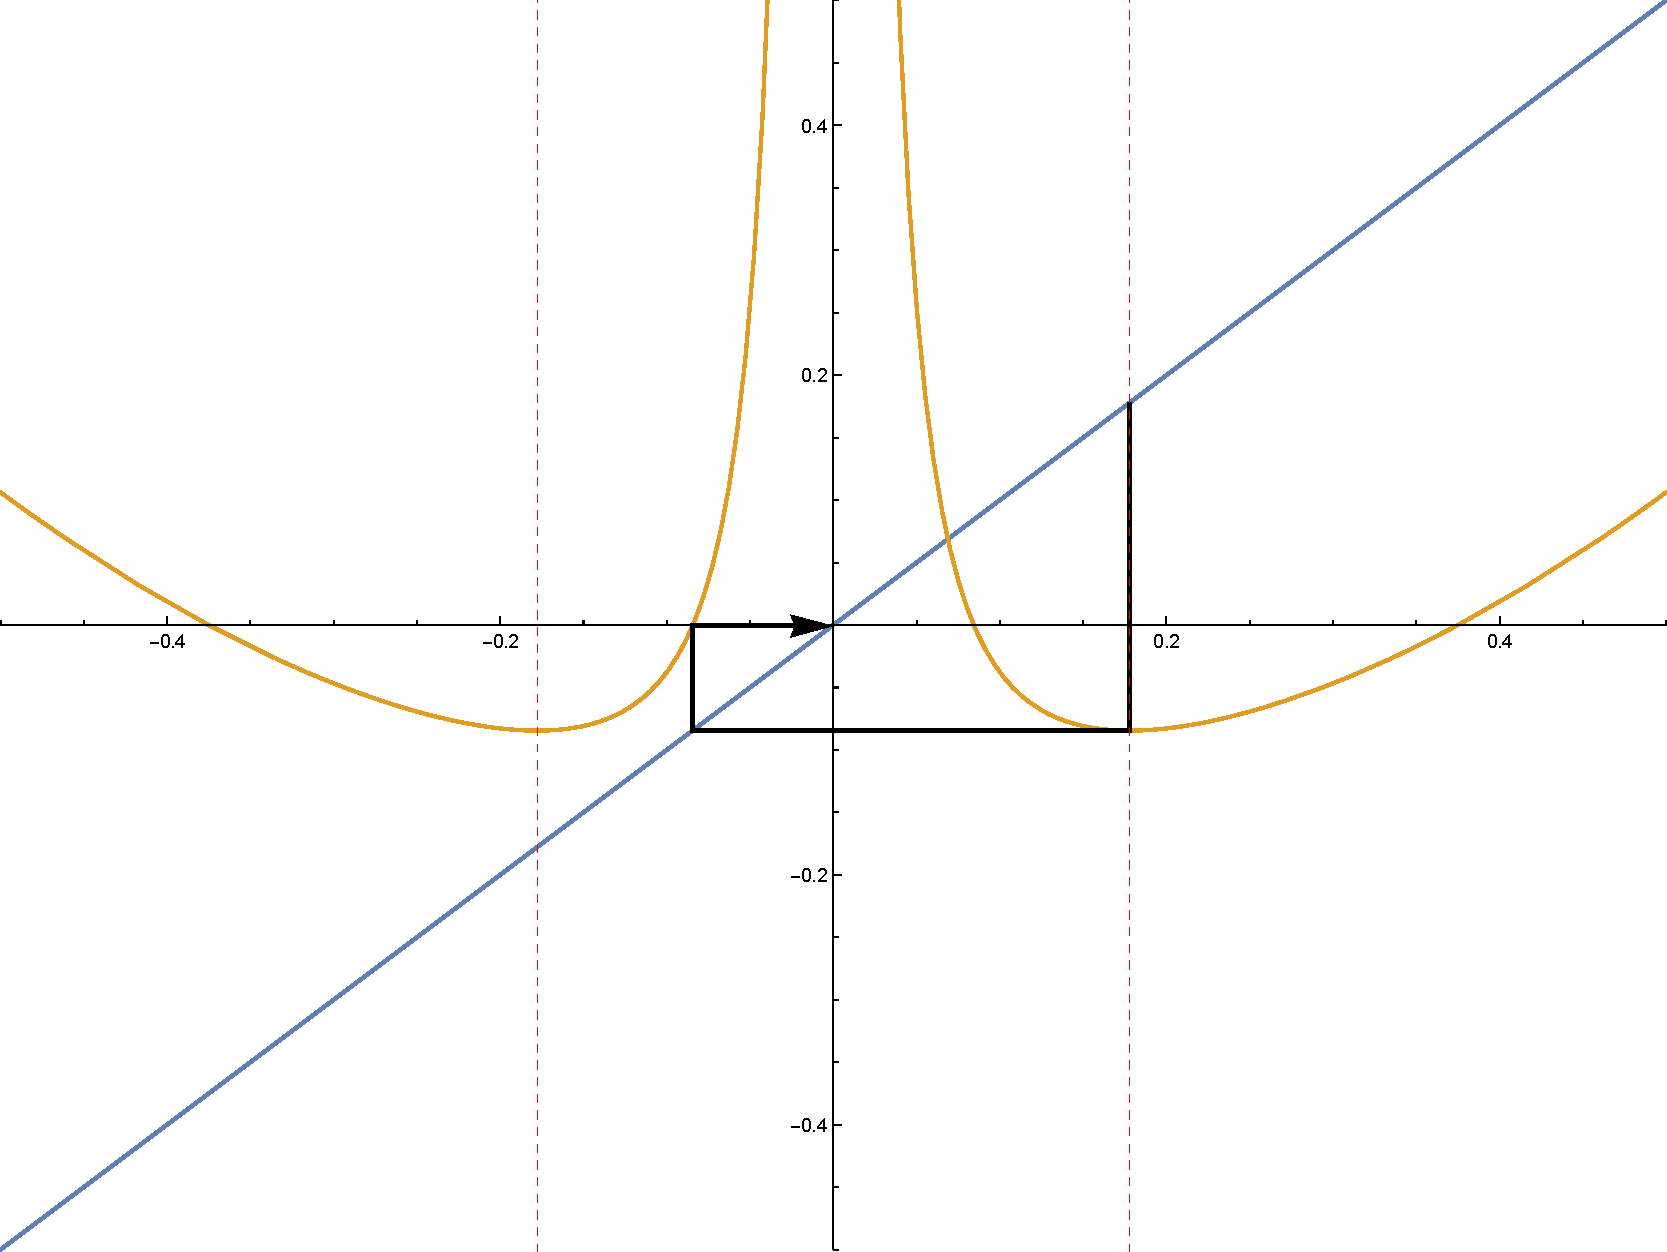
\includegraphics[width=\textwidth]{./img/plot-014778}
				\caption{$c \approx -.14778 \approx z_2^{Cr0}$}
		\end{subfigure}
		% \begin{subfigure}[b]{0.3\textwidth}
		% 		\includegraphics[width=\textwidth]{./img/plot-}
		% 		\caption{Seventh iterate of $f_c (C)$ added along with the parameter value of its prezero orbit}
		% 		\label{fig:cplot6S}
		% \end{subfigure}
		% \begin{subfigure}[b]{0.333\textwidth}
		% 		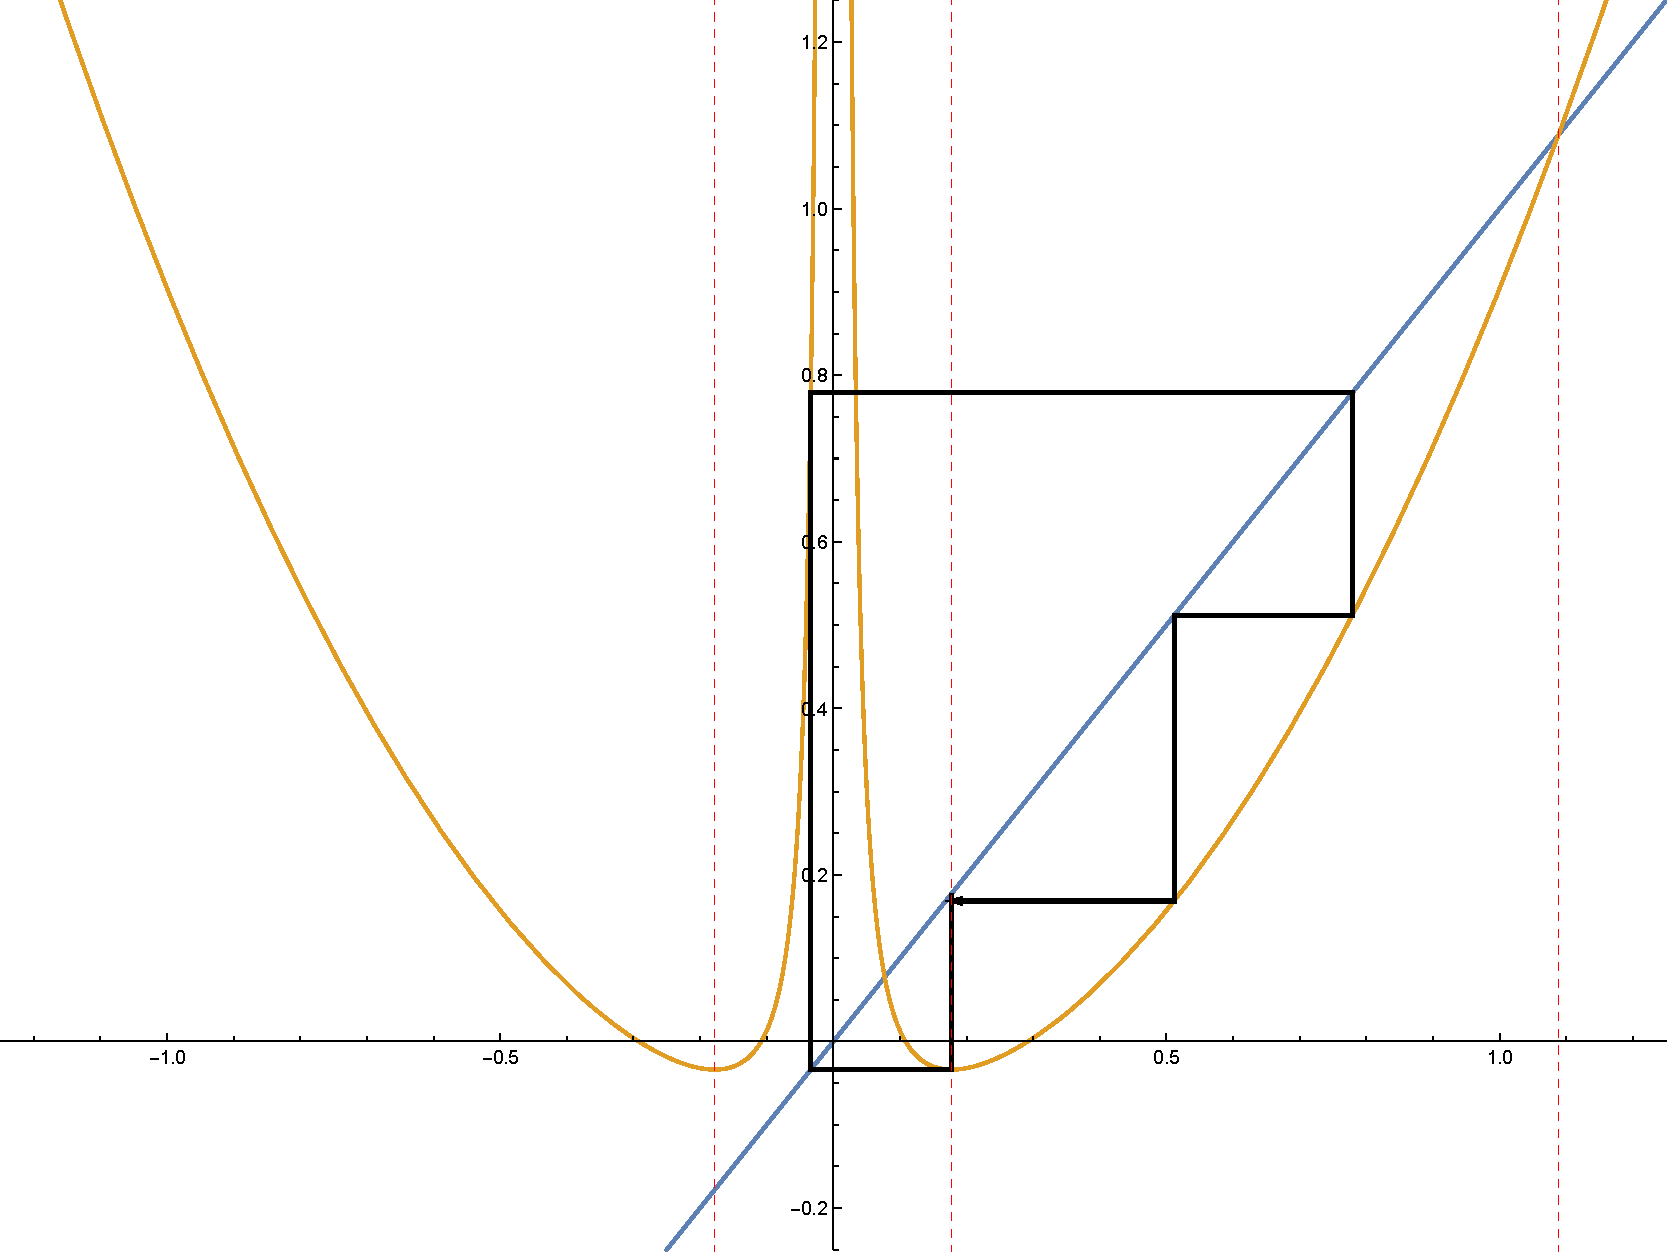
\includegraphics[width=\textwidth]{./img/CrFFC}
		% 		\caption{Seventh iterate of $f_c (C)$ added along with the parameter value of its prezero orbit}
		% 		\label{fig:cplot6S}
		% \end{subfigure}
		 %add desired spacing between images, e. g. ~, \quad, \qquad, \hfill etc.
		  % (or a blank line to force the subfigure onto a new line)
		\caption{Graphical iteration showing the accumulation of periodic, prefixed, and prezero orbits as $c$ approaches $\pl$ (depicted in 3.11 (k)) from the right and the accumulation of periodic, and prezero orbits as $c$ approaches $\pr$ (depicted in 3.10 (e))  from the left}\label{fig:giters}
\end{figure}

\begin{figure}[ht]
		\centering
		\begin{subfigure}[b]{0.3\textwidth}
				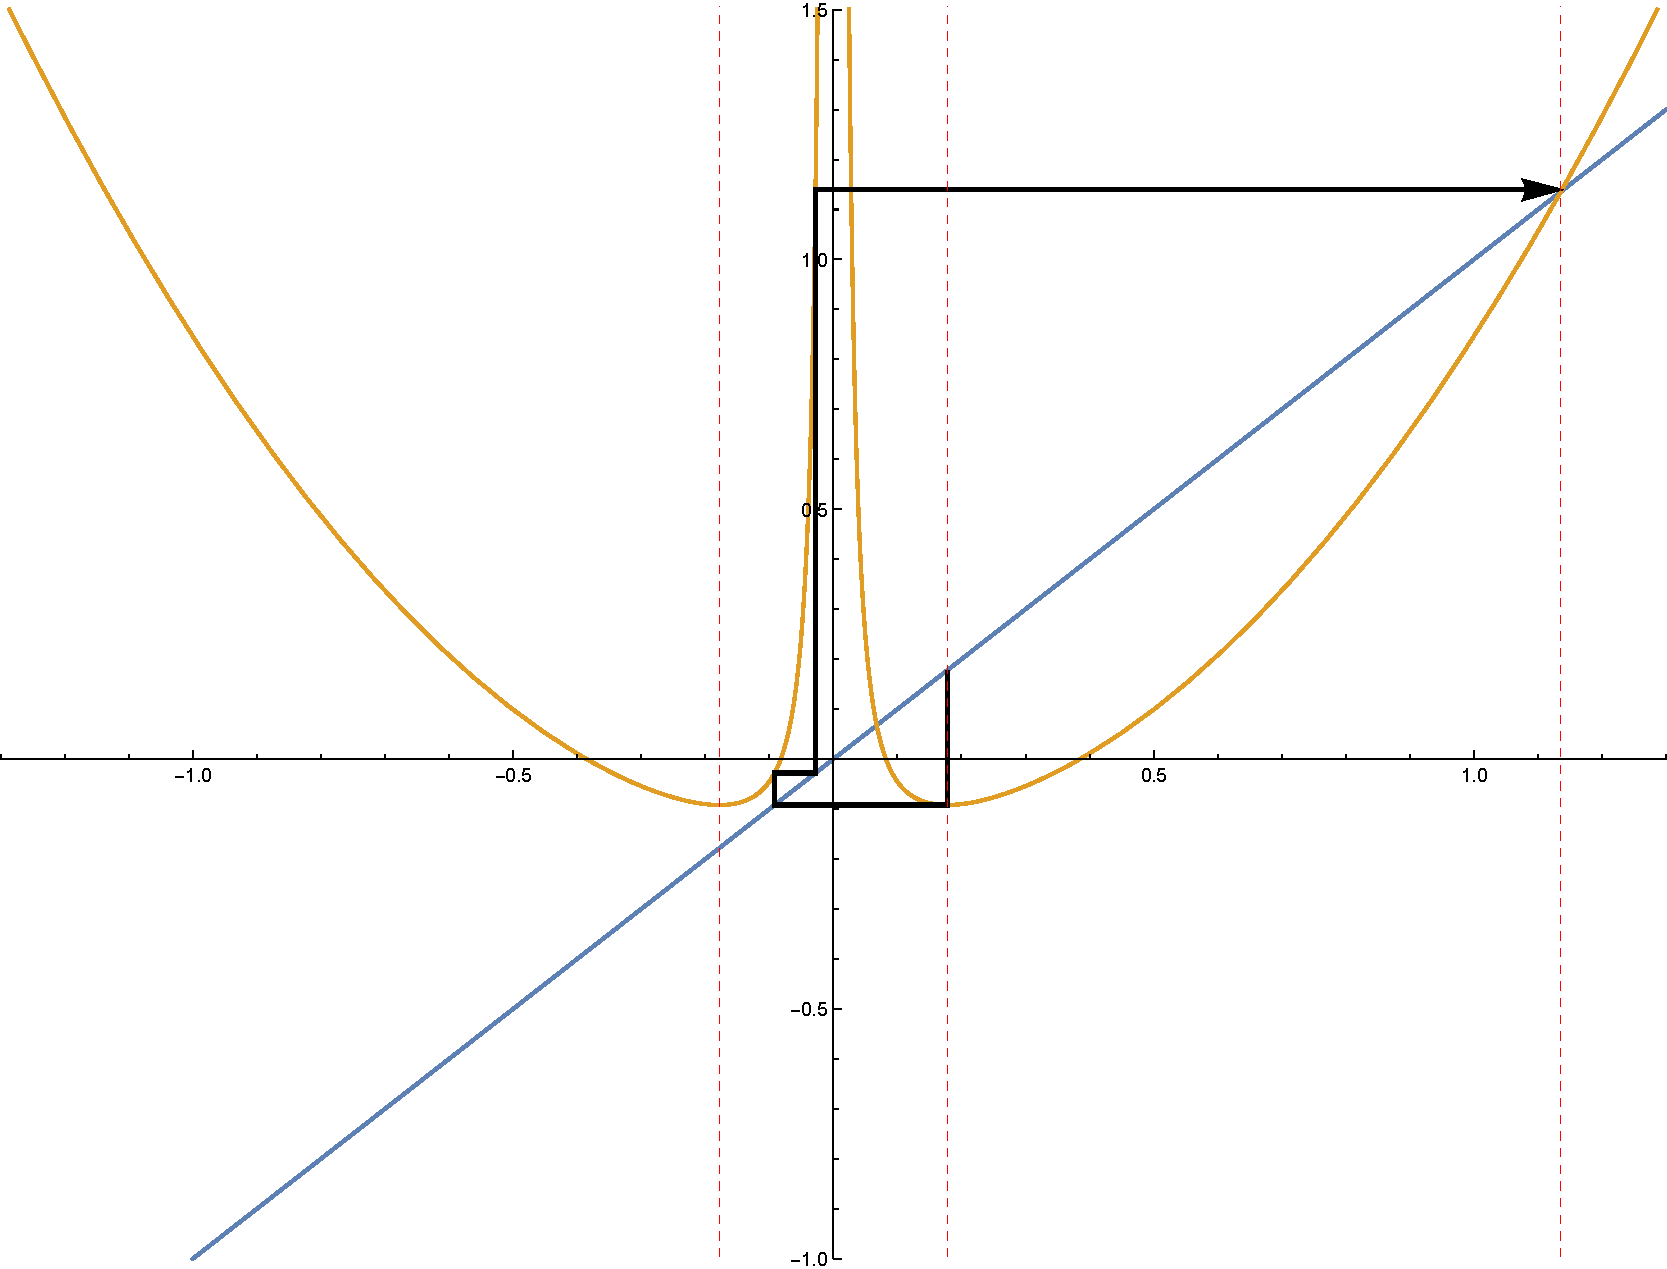
\includegraphics[width=\textwidth]{./img/plot-0155}
				\caption{$c \approx -.155 \approx h_3^{CrrP_c}$}
		\end{subfigure}
		\begin{subfigure}[b]{0.3\textwidth}
				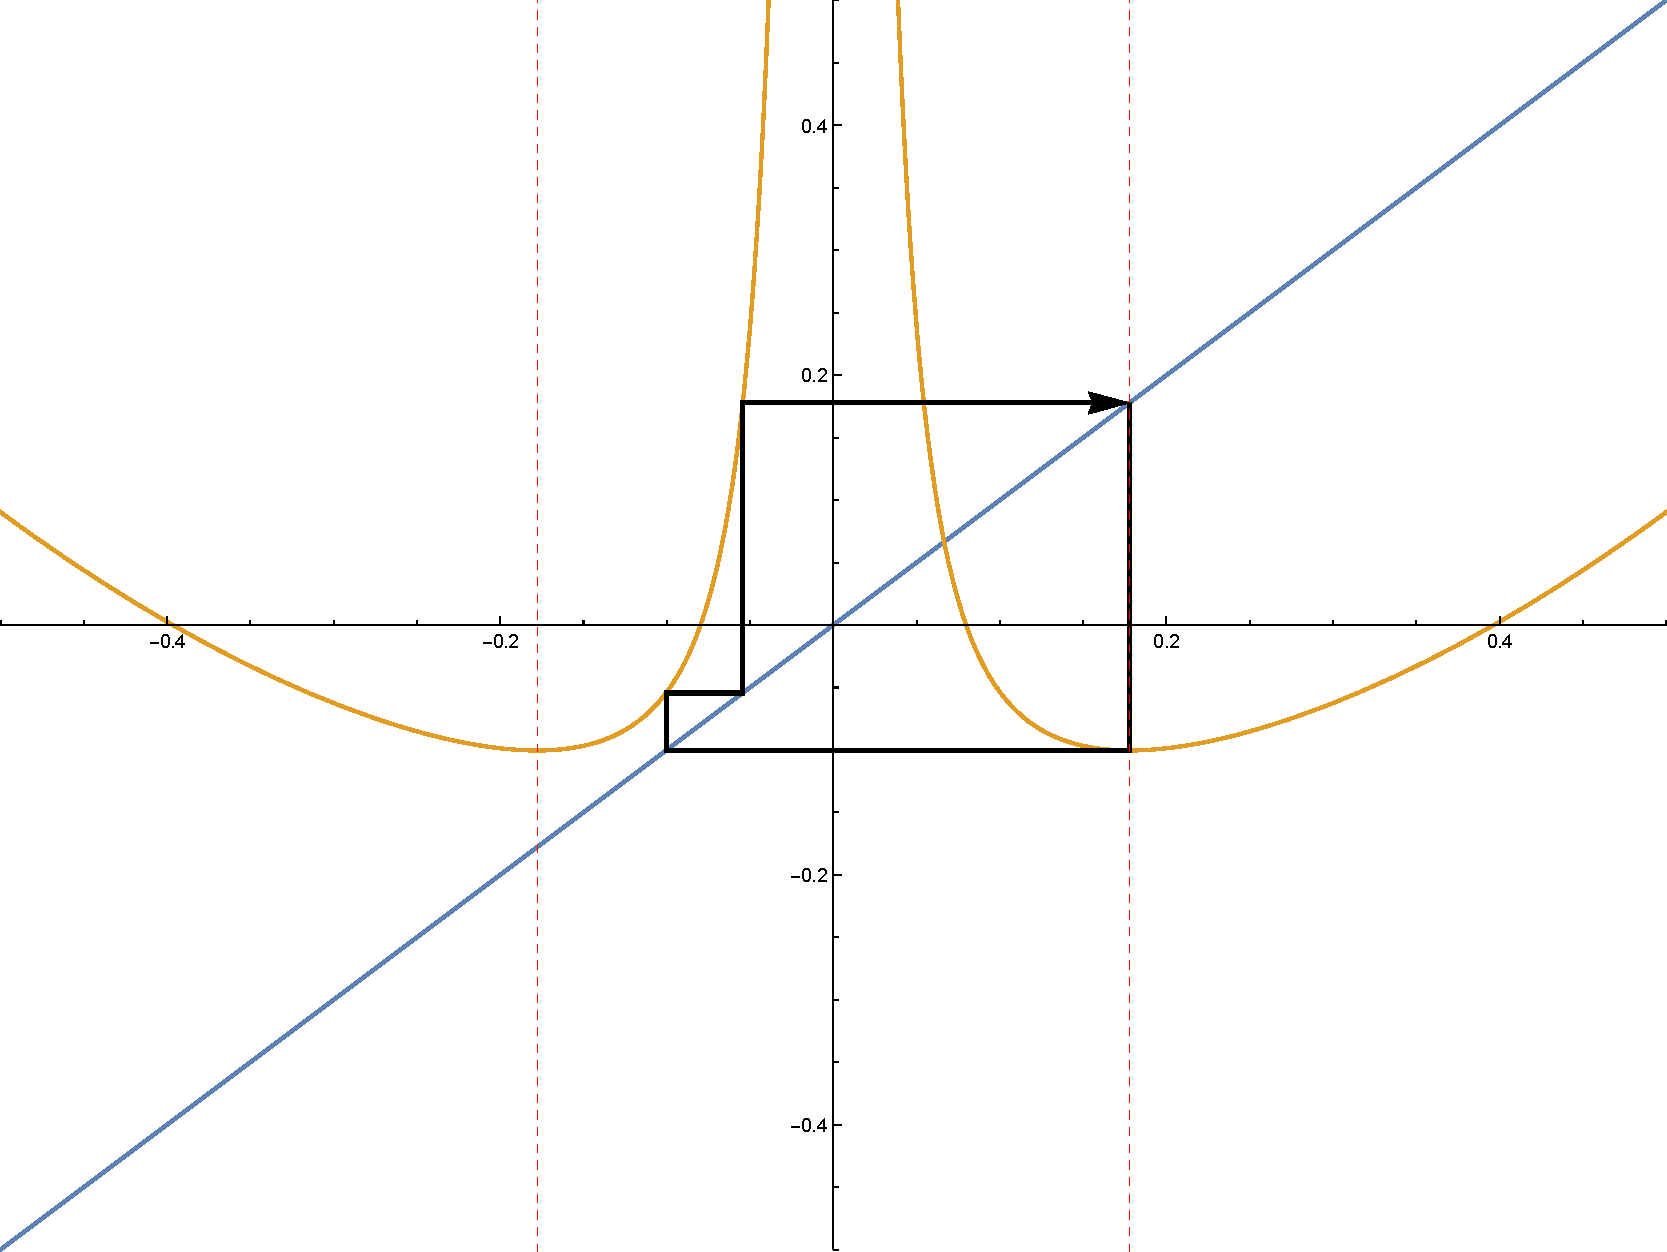
\includegraphics[width=\textwidth]{./img/plot-016364}
				\caption{$c \approx - .16364 \approx p_3^{CrrC}$}
		\end{subfigure}
		\begin{subfigure}[b]{0.3\textwidth}
				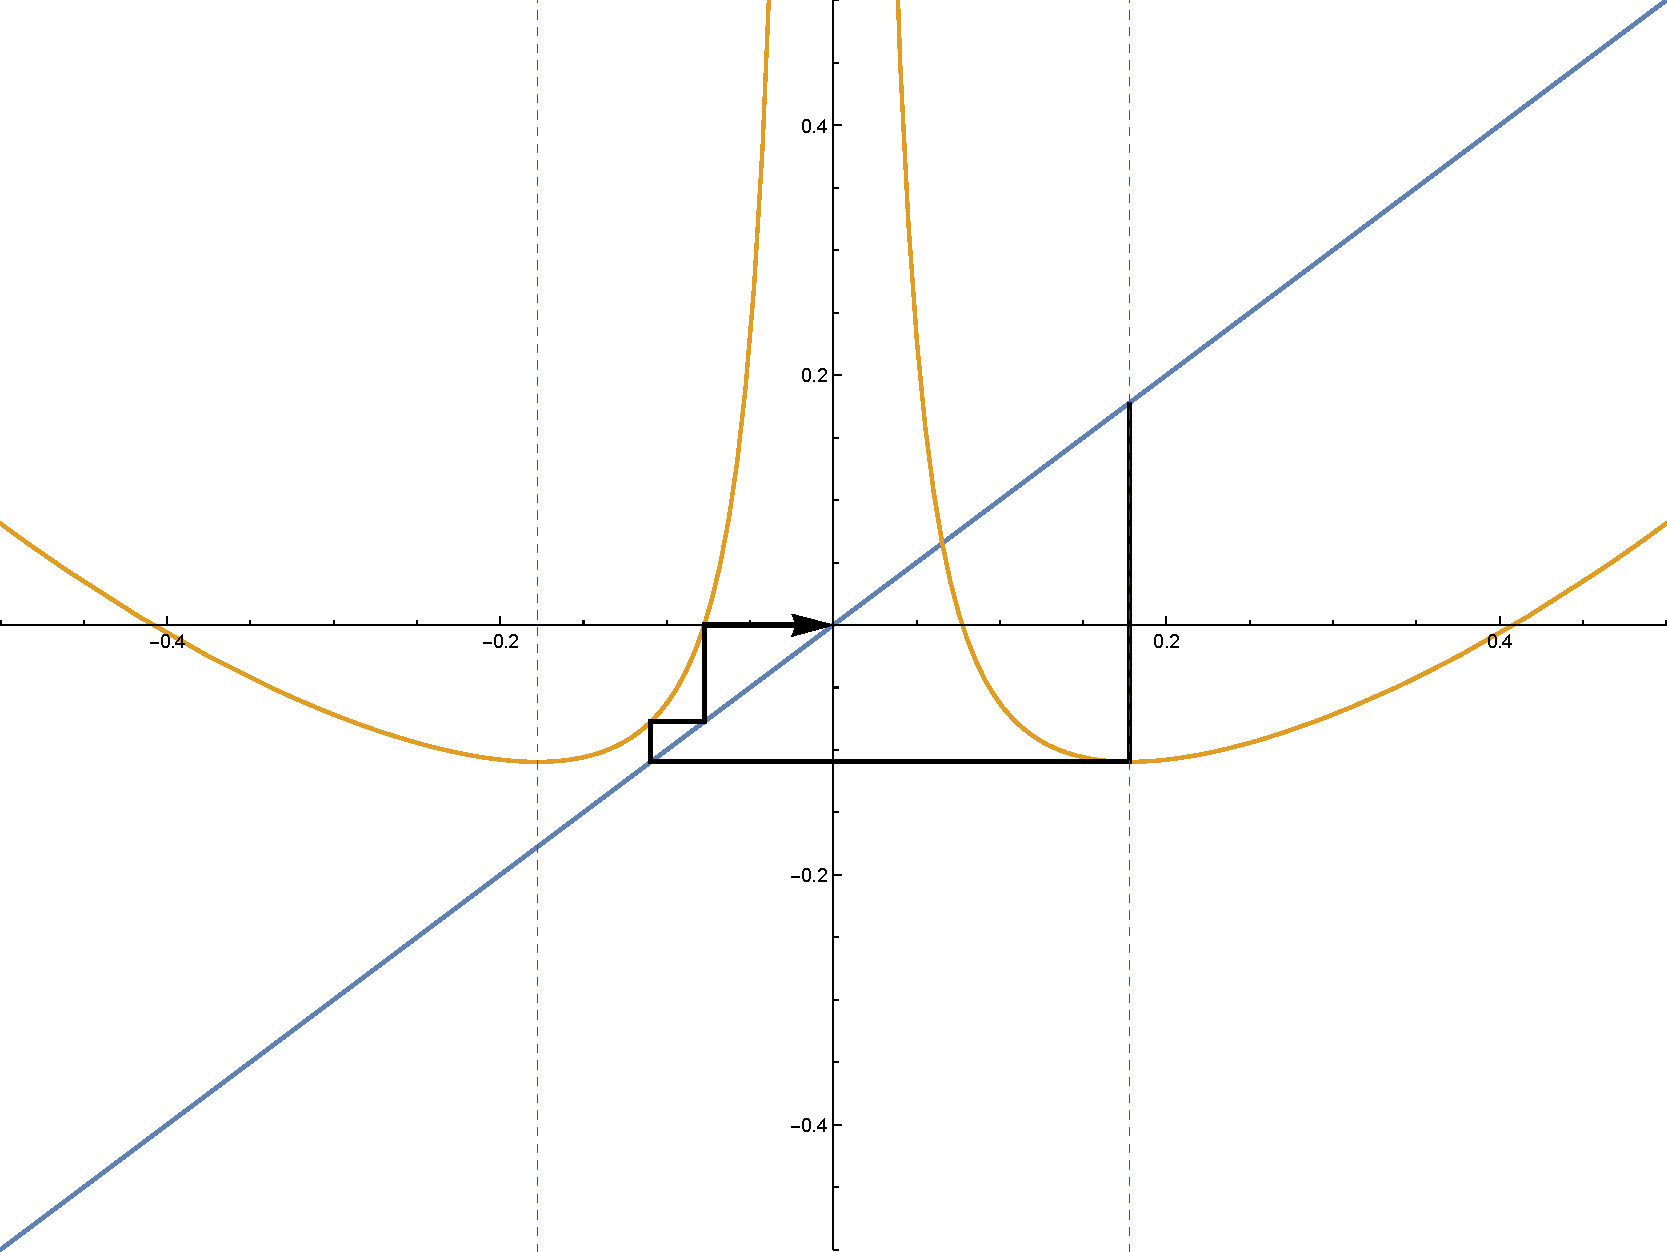
\includegraphics[width=\textwidth]{./img/plot-017278}
				\caption{$c \approx -.17278 \approx z_3^{Crr0}$}
		\end{subfigure}

		\begin{subfigure}[b]{0.3\textwidth}
				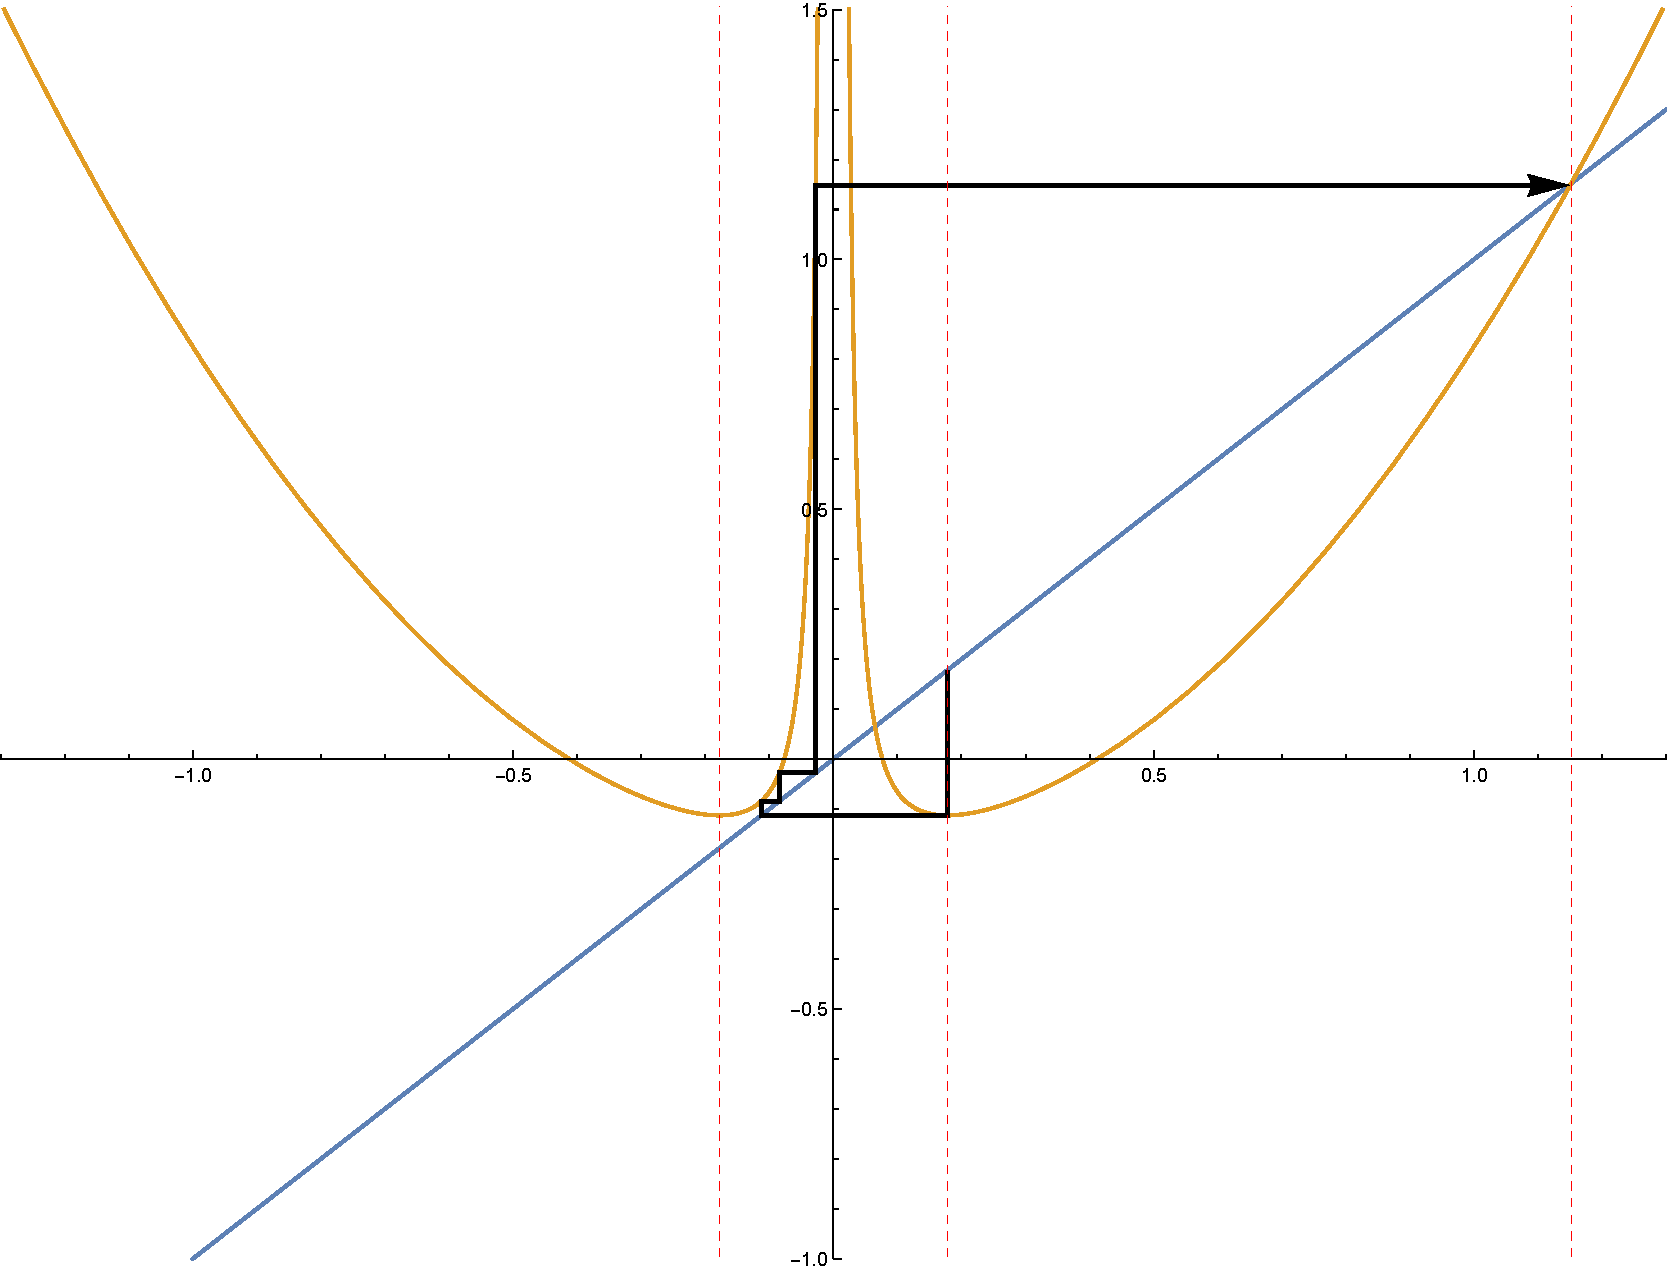
\includegraphics[width=\textwidth]{./img/plot-017578}
				\caption{$c \approx -.17578 \approx h_4^{CrrrP_c}$}
		\end{subfigure}
		\begin{subfigure}[b]{0.3\textwidth}
				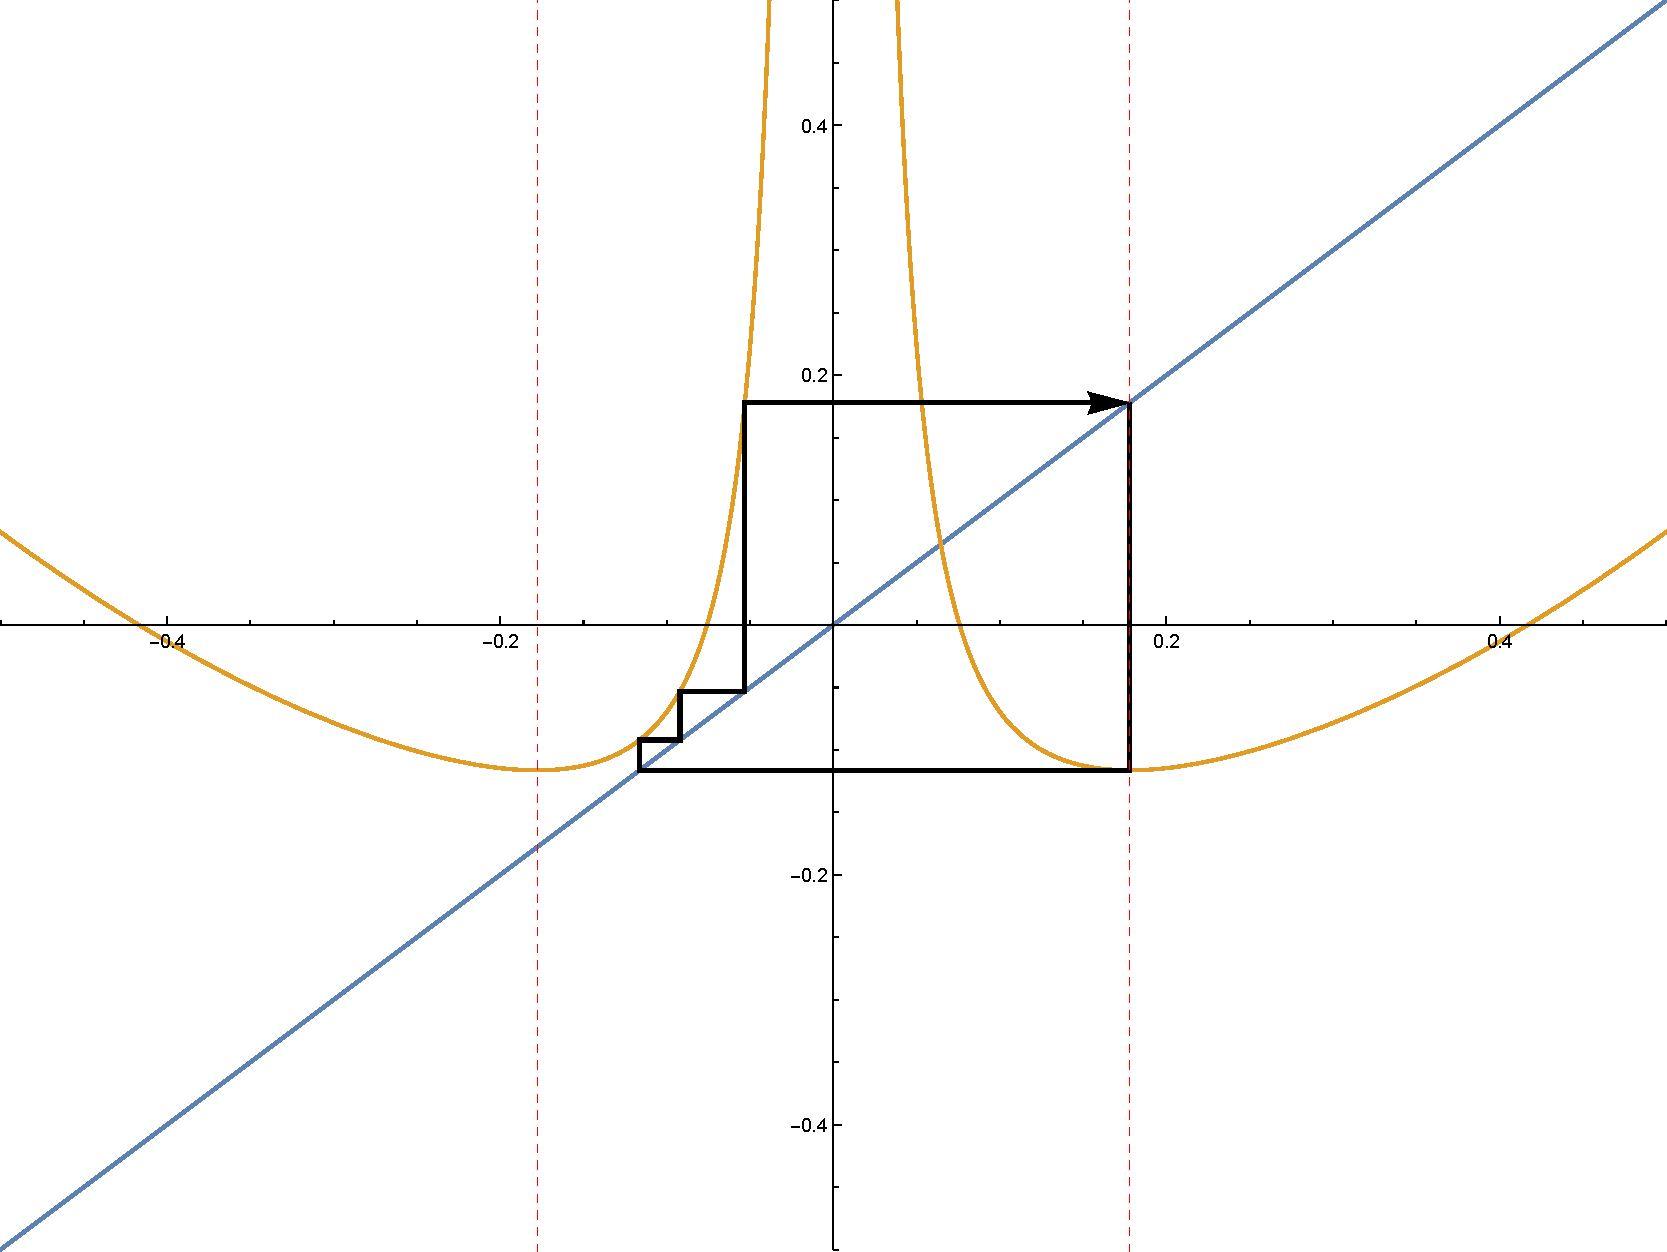
\includegraphics[width=\textwidth]{./img/plot-017954}
				\caption{$c \approx - .17954 \approx p_4^{CrrrC}$}
		\end{subfigure}
		\begin{subfigure}[b]{0.3\textwidth}
				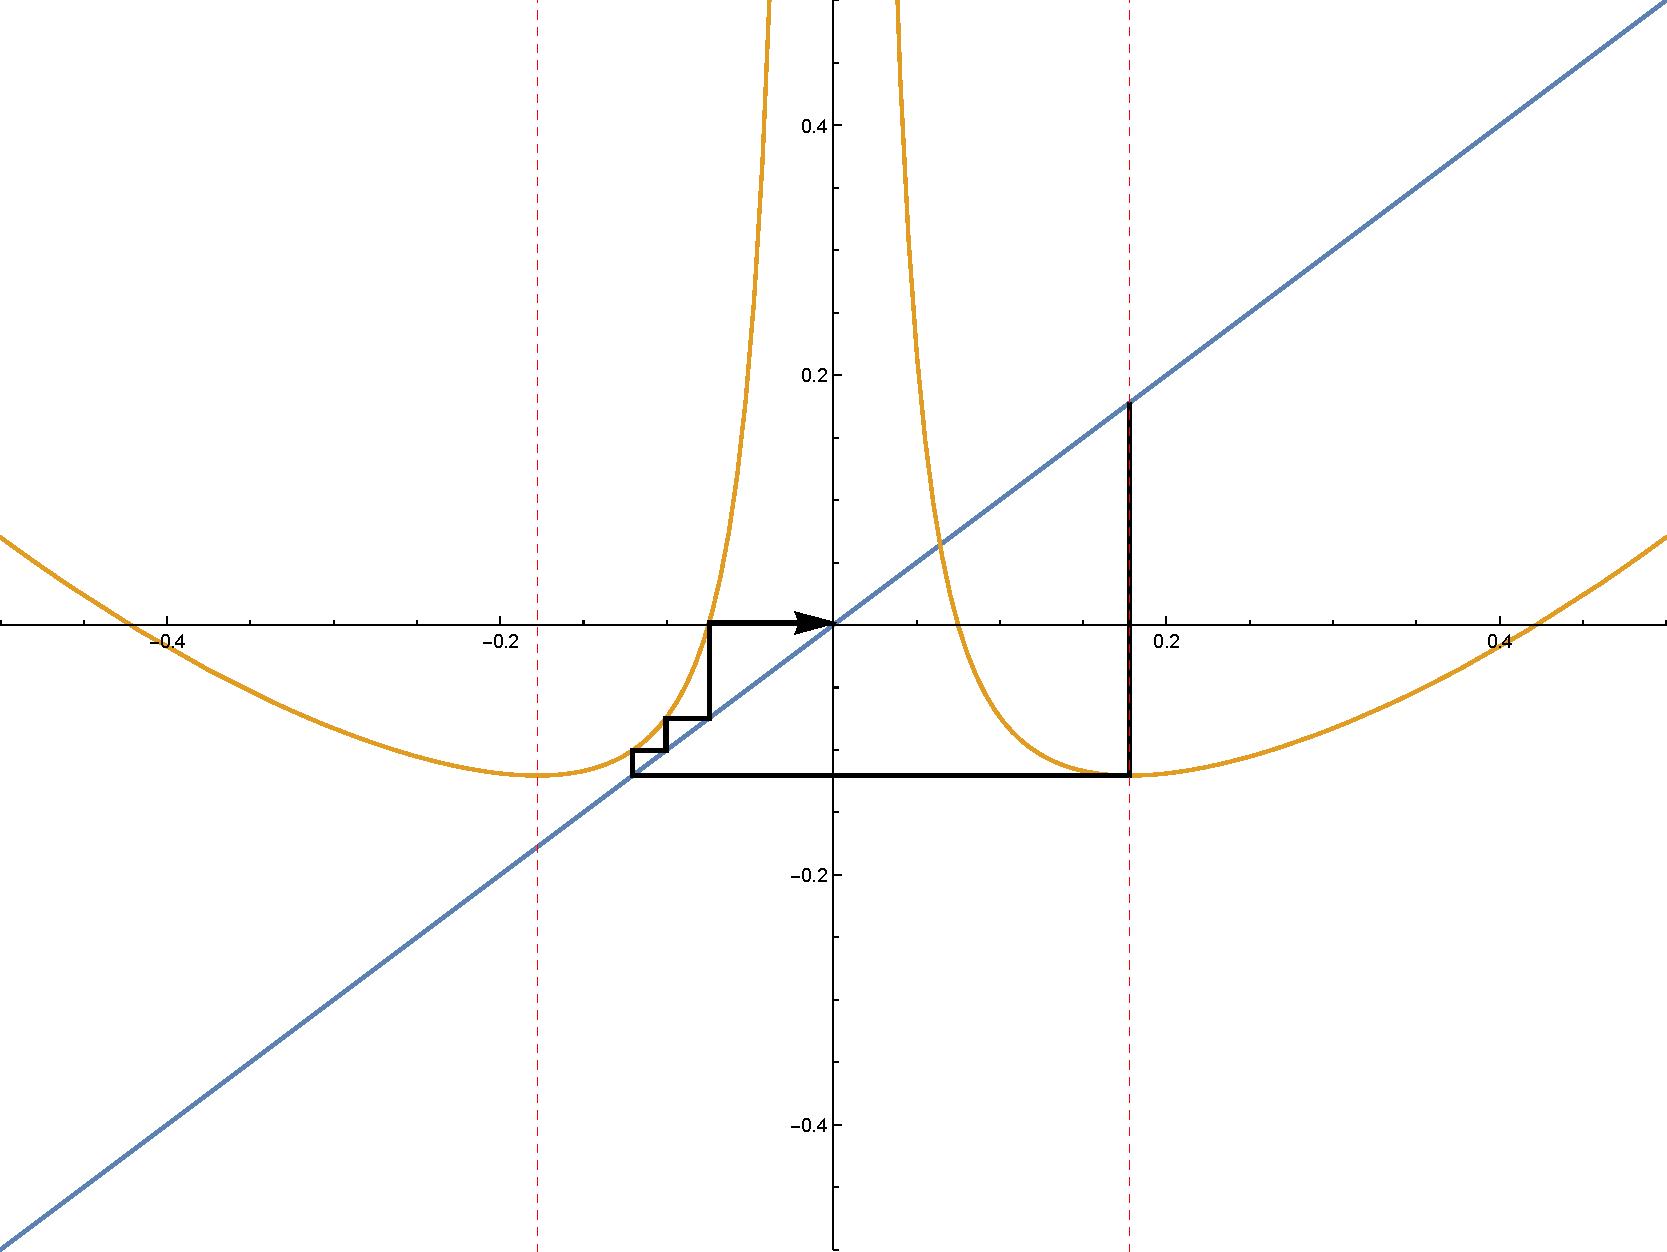
\includegraphics[width=\textwidth]{./img/plot-018378}
				\caption{$c \approx -.18378 \approx z_4^{Crrr0}$}
		\end{subfigure}

		\begin{subfigure}[b]{0.3\textwidth}
				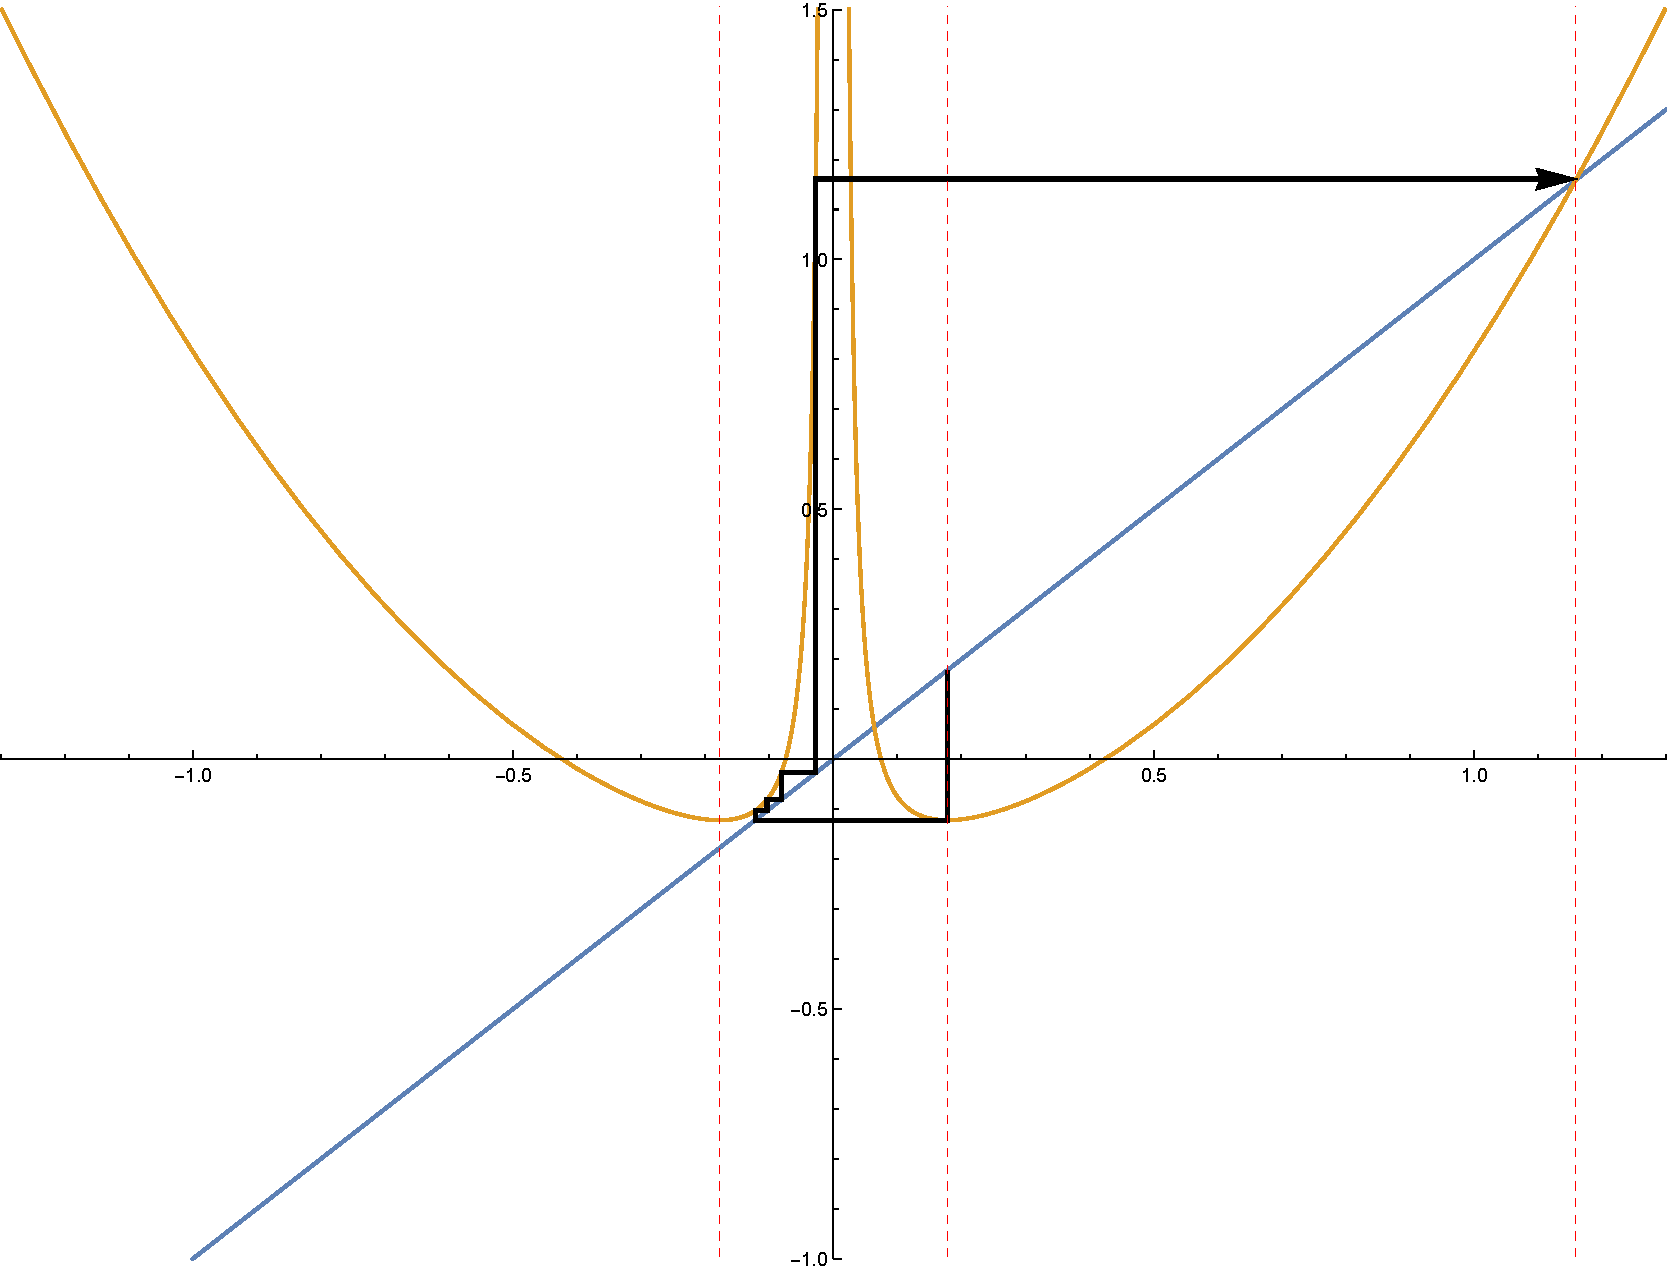
\includegraphics[width=\textwidth]{./img/plot-018539}
				\caption{$c \approx -.18539 \approx h_5^{CrrrrP_c}$}
		\end{subfigure}
		\begin{subfigure}[b]{0.3\textwidth}
				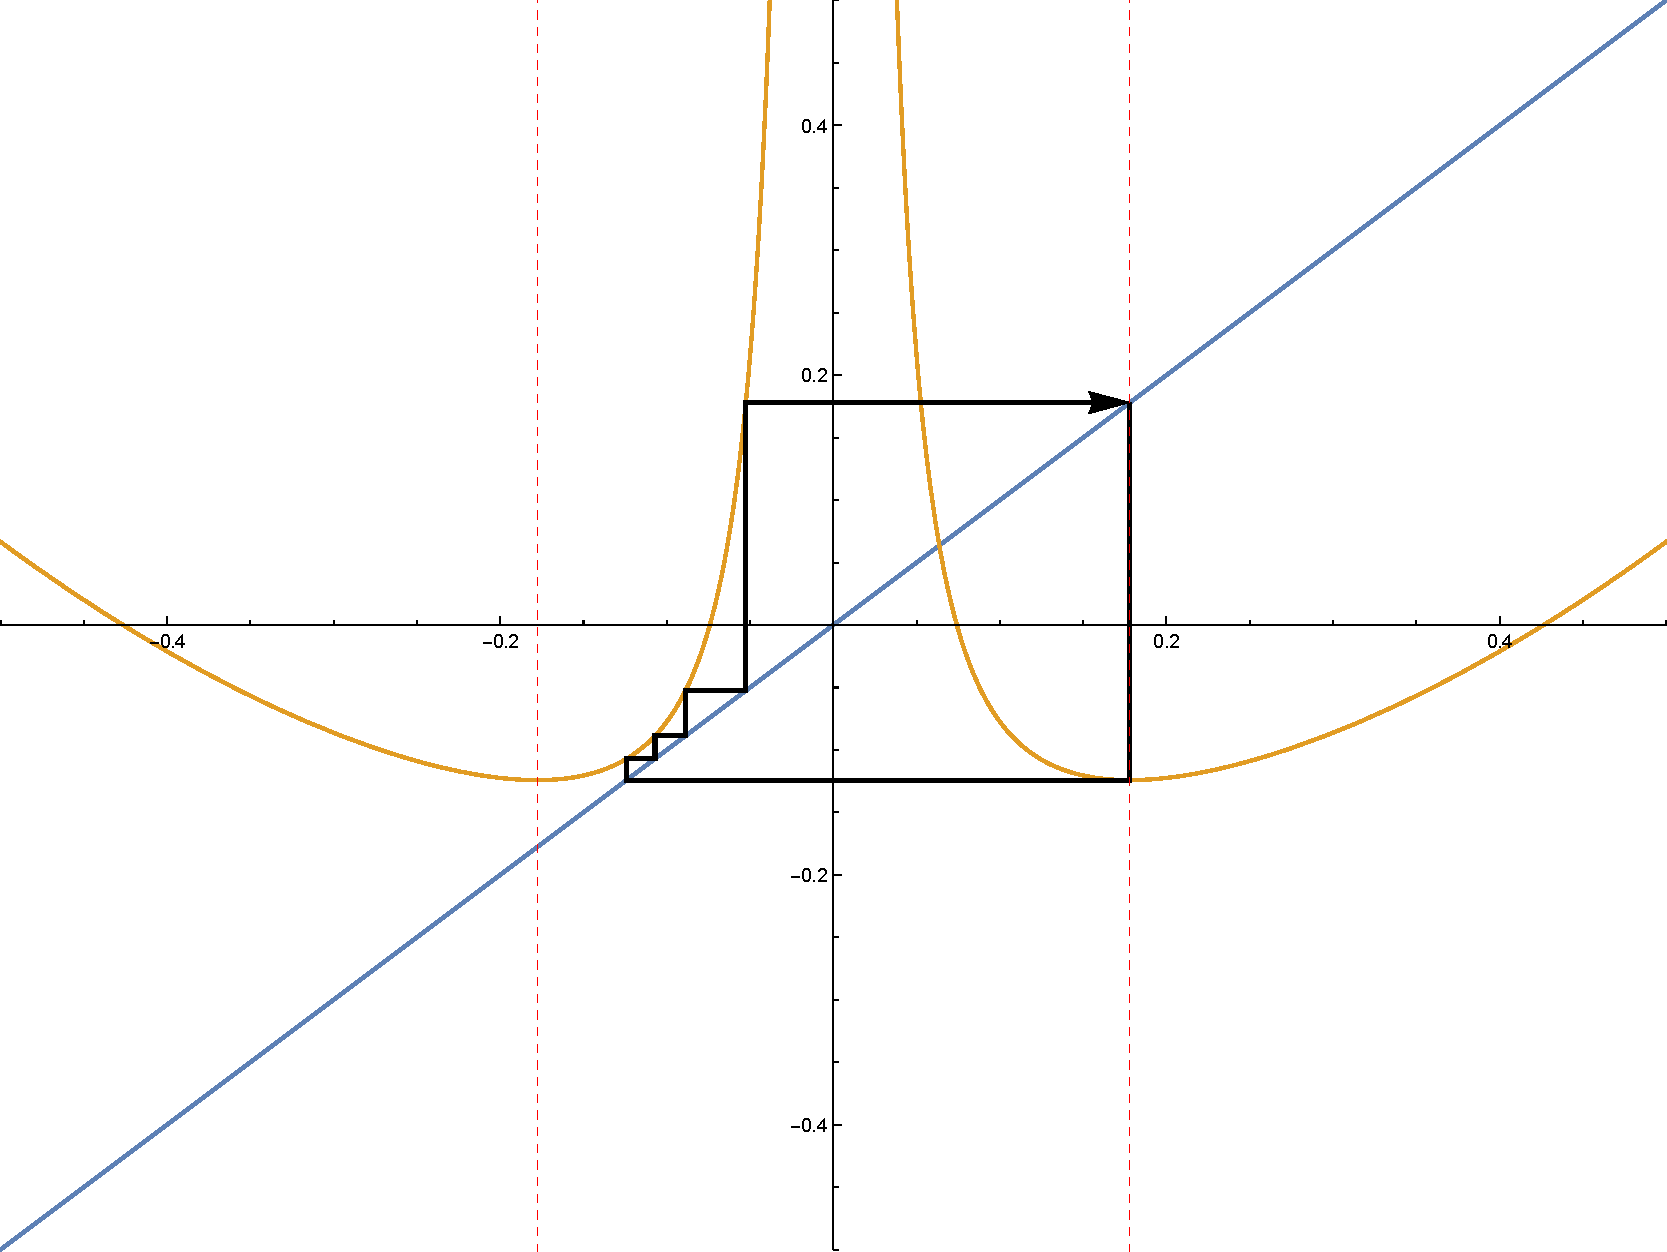
\includegraphics[width=\textwidth]{./img/plot-018739}
				\caption{$c \approx - .18739\approx p_5^{CrrrrC}$}
		\end{subfigure}
		\begin{subfigure}[b]{0.3\textwidth}
				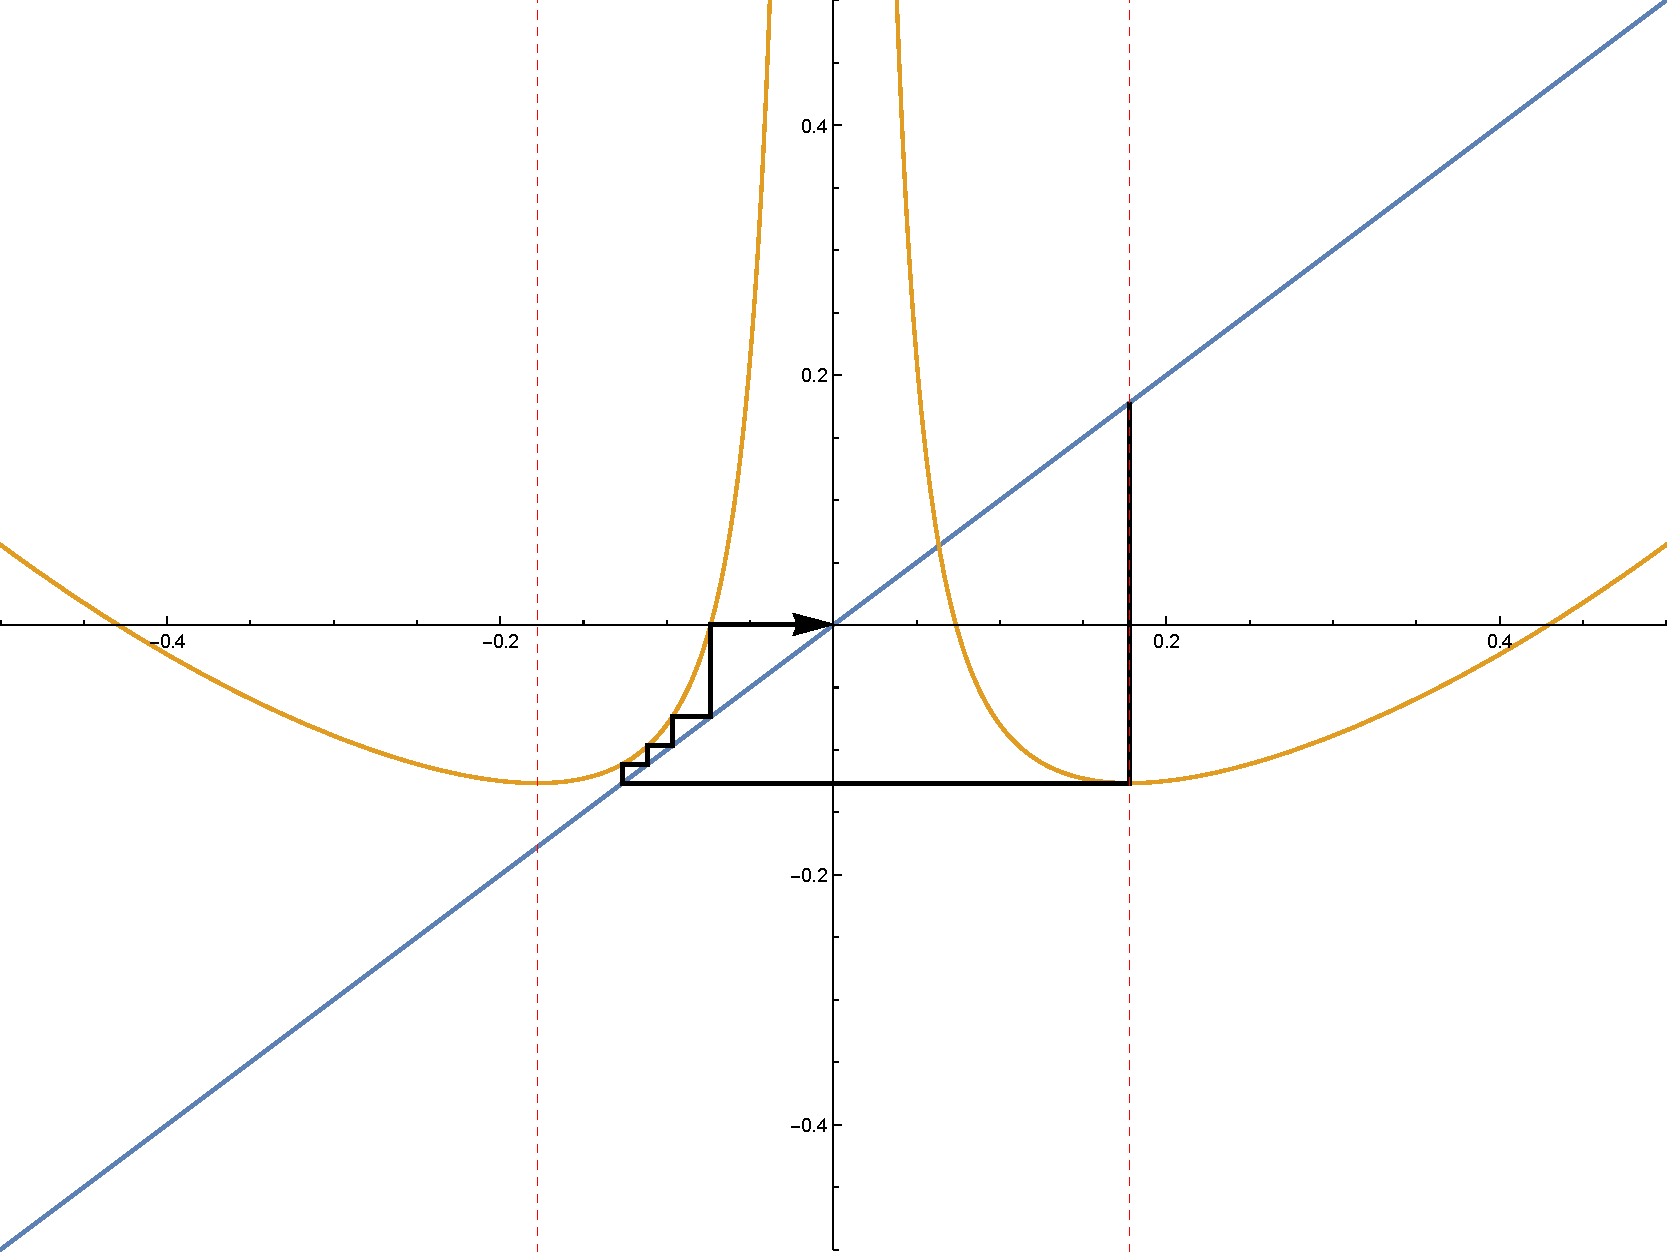
\includegraphics[width=\textwidth]{./img/plot-018979}
				\caption{$c \approx - .18979 \approx z_5^{Crrrr0}$}
		\end{subfigure}

		\begin{subfigure}[b]{0.3\textwidth}
				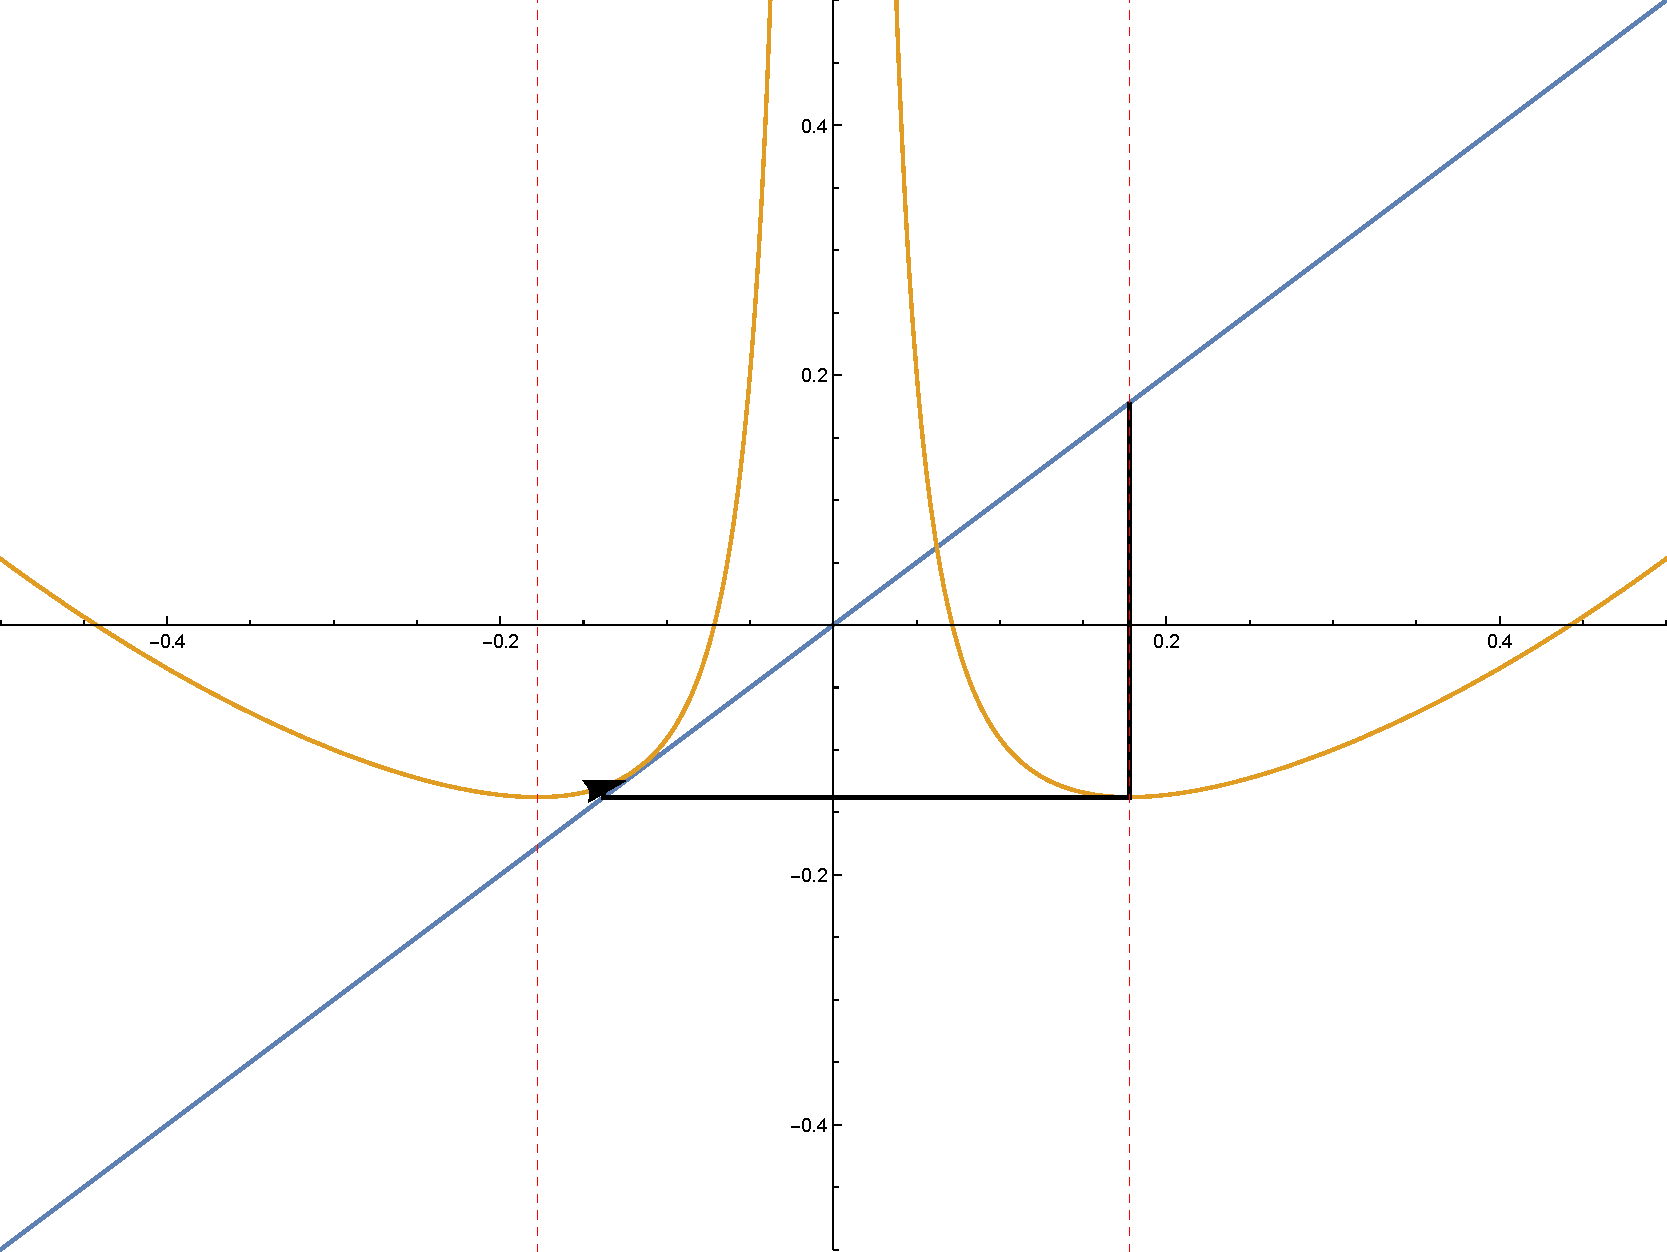
\includegraphics[width=\textwidth]{./img/plot-0201}
				\caption{$c \approx - .201\approx s_1^l$}
		\end{subfigure}
		\begin{subfigure}[b]{0.3\textwidth}
				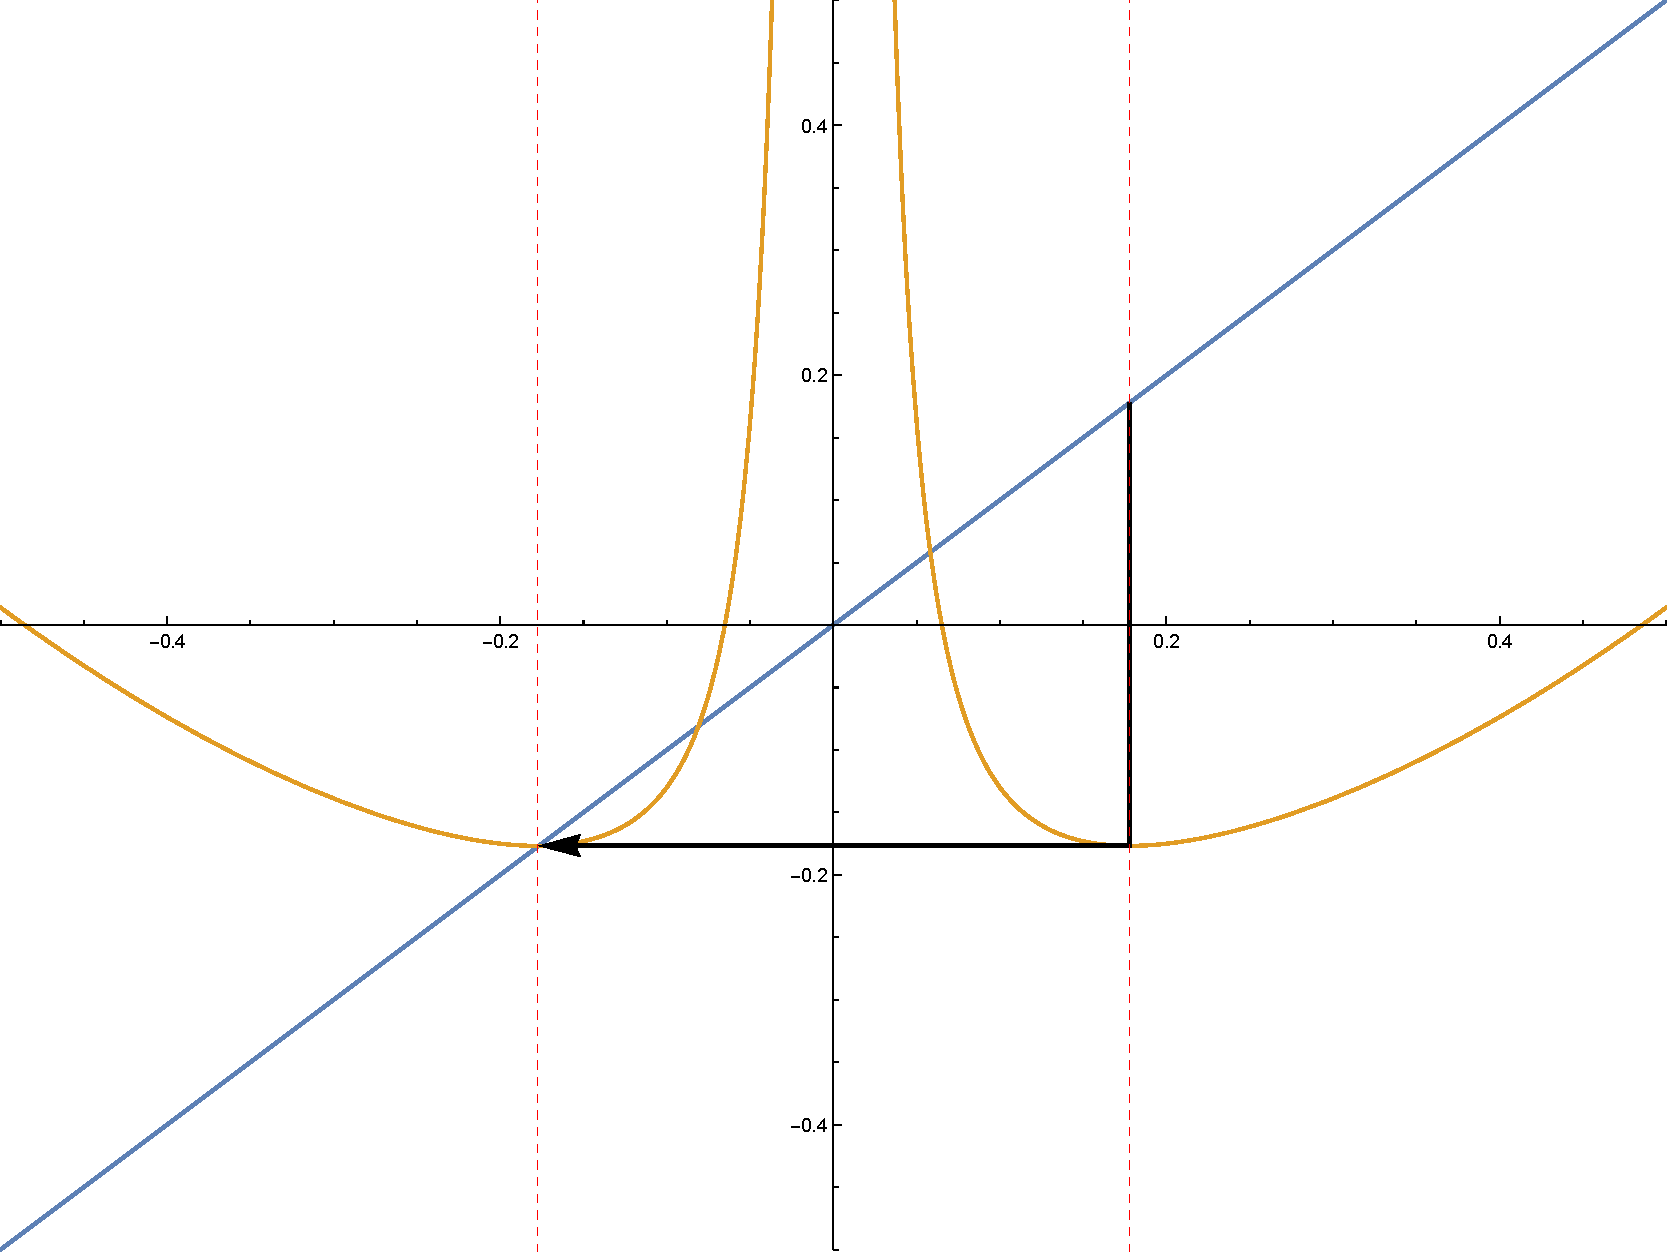
\includegraphics[width=\textwidth]{./img/plot-024}
				\caption{$c \approx -.24 \approx p_1^{-C}$}
		\end{subfigure}
		% \begin{subfigure}[b]{0.3\textwidth}
		% 		\includegraphics[width=\textwidth]{./img/plot-}
		% 		\caption{Seventh iterate of $f_c (C)$ added along with the parameter value of its prezero orbit}
		% 		\label{fig:cplot6S}
		% \end{subfigure}
		% \begin{subfigure}[b]{0.333\textwidth}
		% 		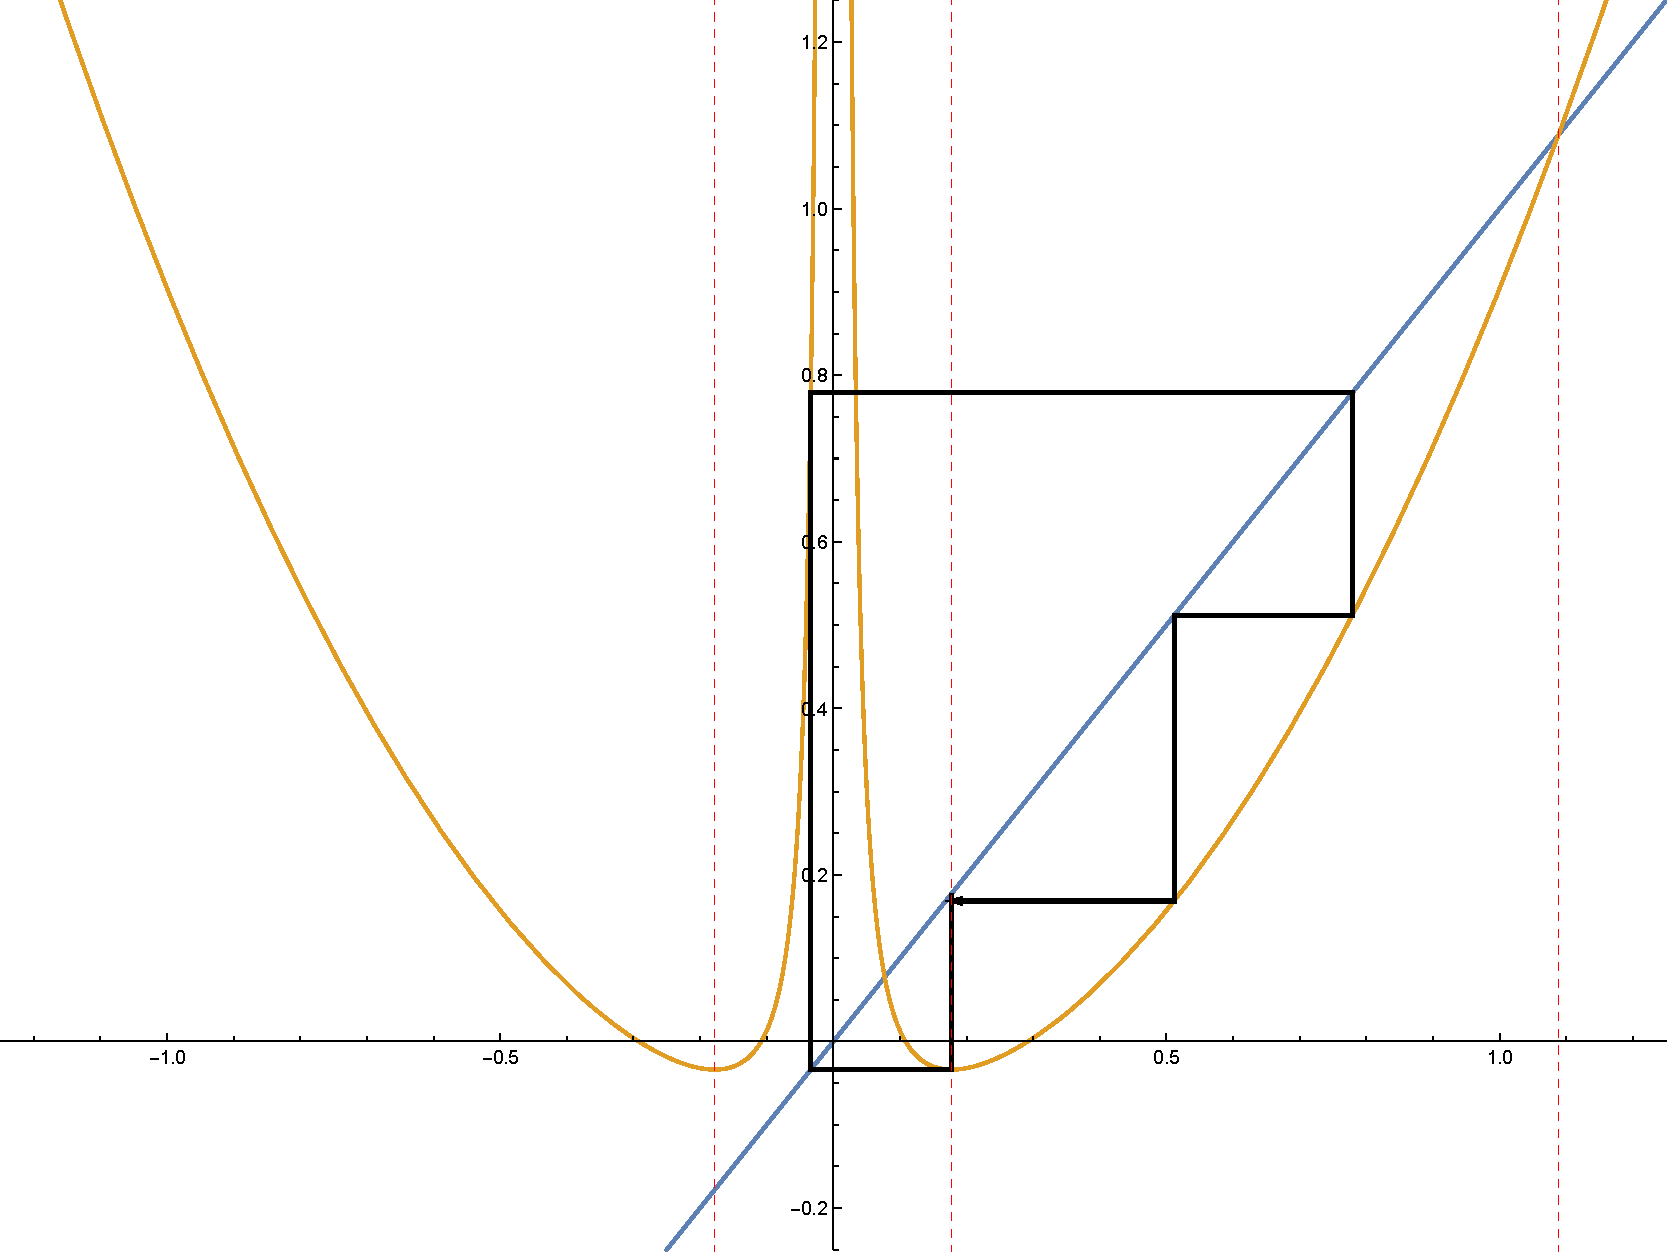
\includegraphics[width=\textwidth]{./img/CrFFC}
		% 		\caption{Seventh iterate of $f_c (C)$ added along with the parameter value of its prezero orbit}
		% 		\label{fig:cplot6S}
		% \end{subfigure}
		 %add desired spacing between images, e. g. ~, \quad, \qquad, \hfill etc.
		  % (or a blank line to force the subfigure onto a new line)
		\caption{Graphical iteration showing the accumulation of periodic, prefixed, and prezero orbits as $c$ approaches $\pl$ (depicted in 3.11 (k)) from the right and the accumulation of periodic, and prezero orbits as $c$ approaches $\pr$ (depicted in 3.10 (e))  from the left (continued)}\label{fig:giters2}
\end{figure}

\begin{figure}[ht]
		\centering
		\begin{subfigure}[b]{0.5\textwidth}
				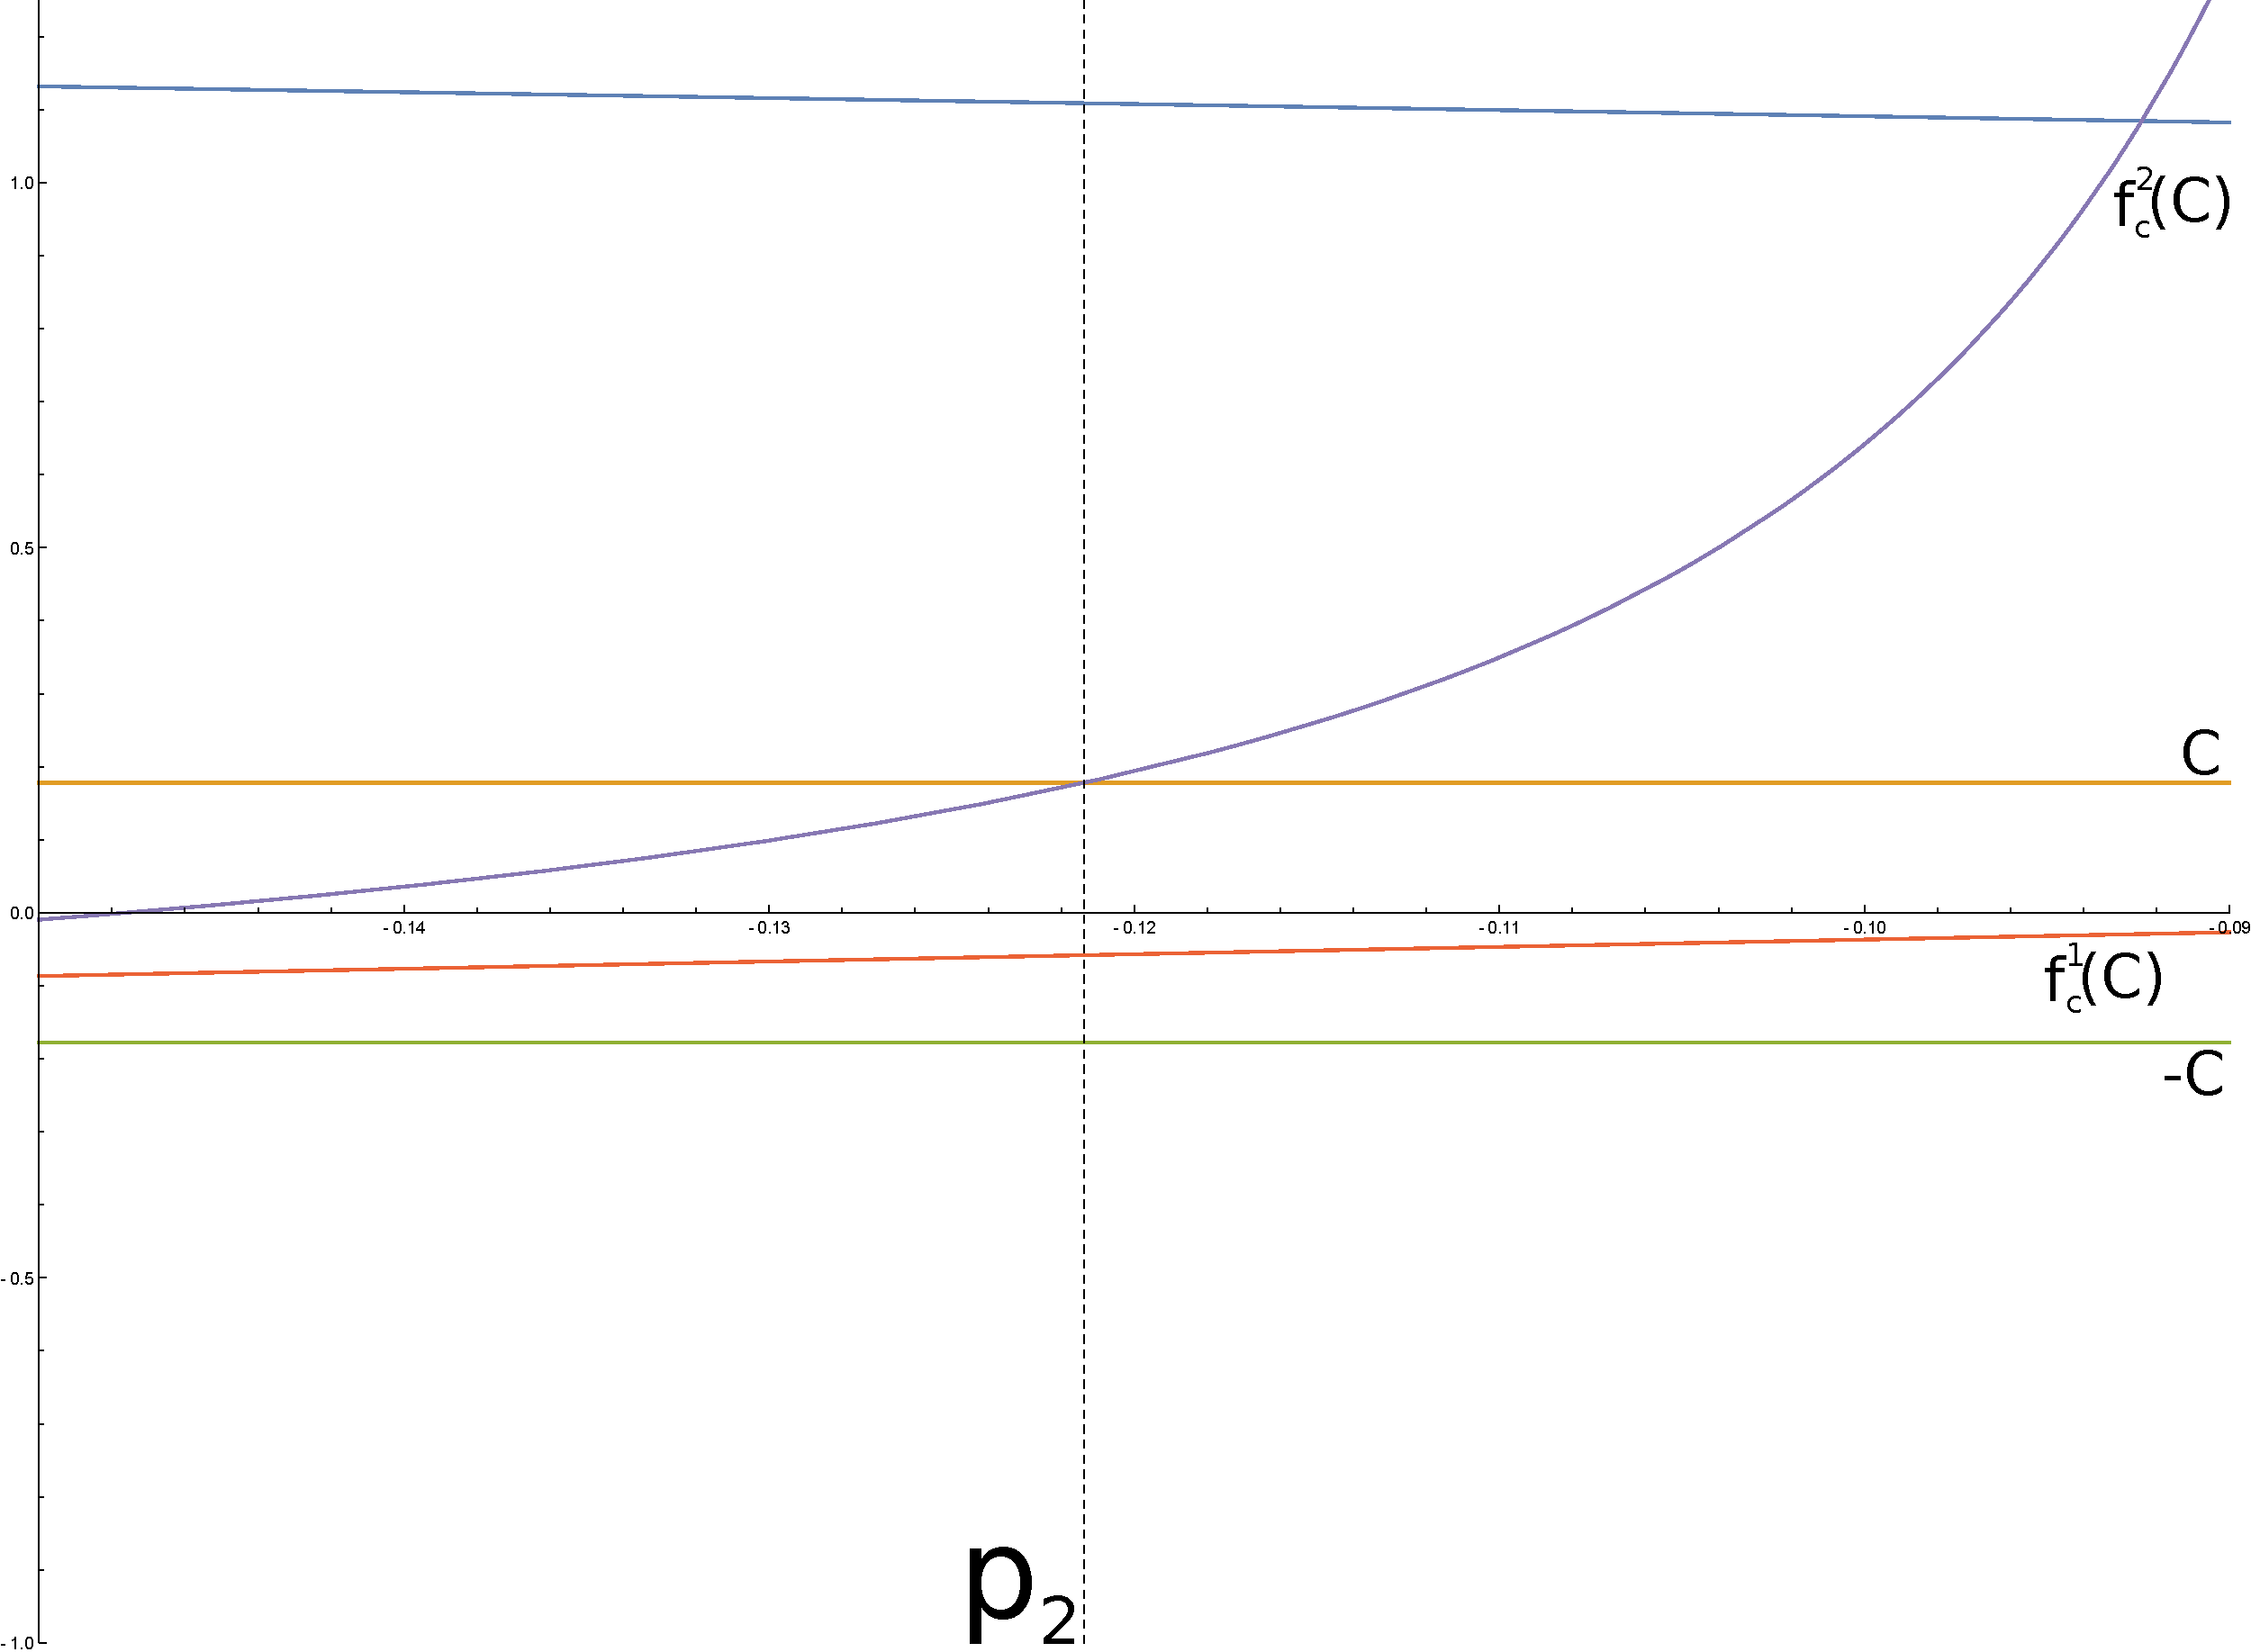
\includegraphics[width=\textwidth]{./img/cplot1H}
				\caption{$n = 2$}
				\label{fig:cplot1H}
		\end{subfigure}%
		~ %add desired spacing between images, e. g. ~, \quad, \qquad, \hfill etc.
		  % (or a blank line to force the subfigure onto a new line)
		\begin{subfigure}[b]{0.5\textwidth}
				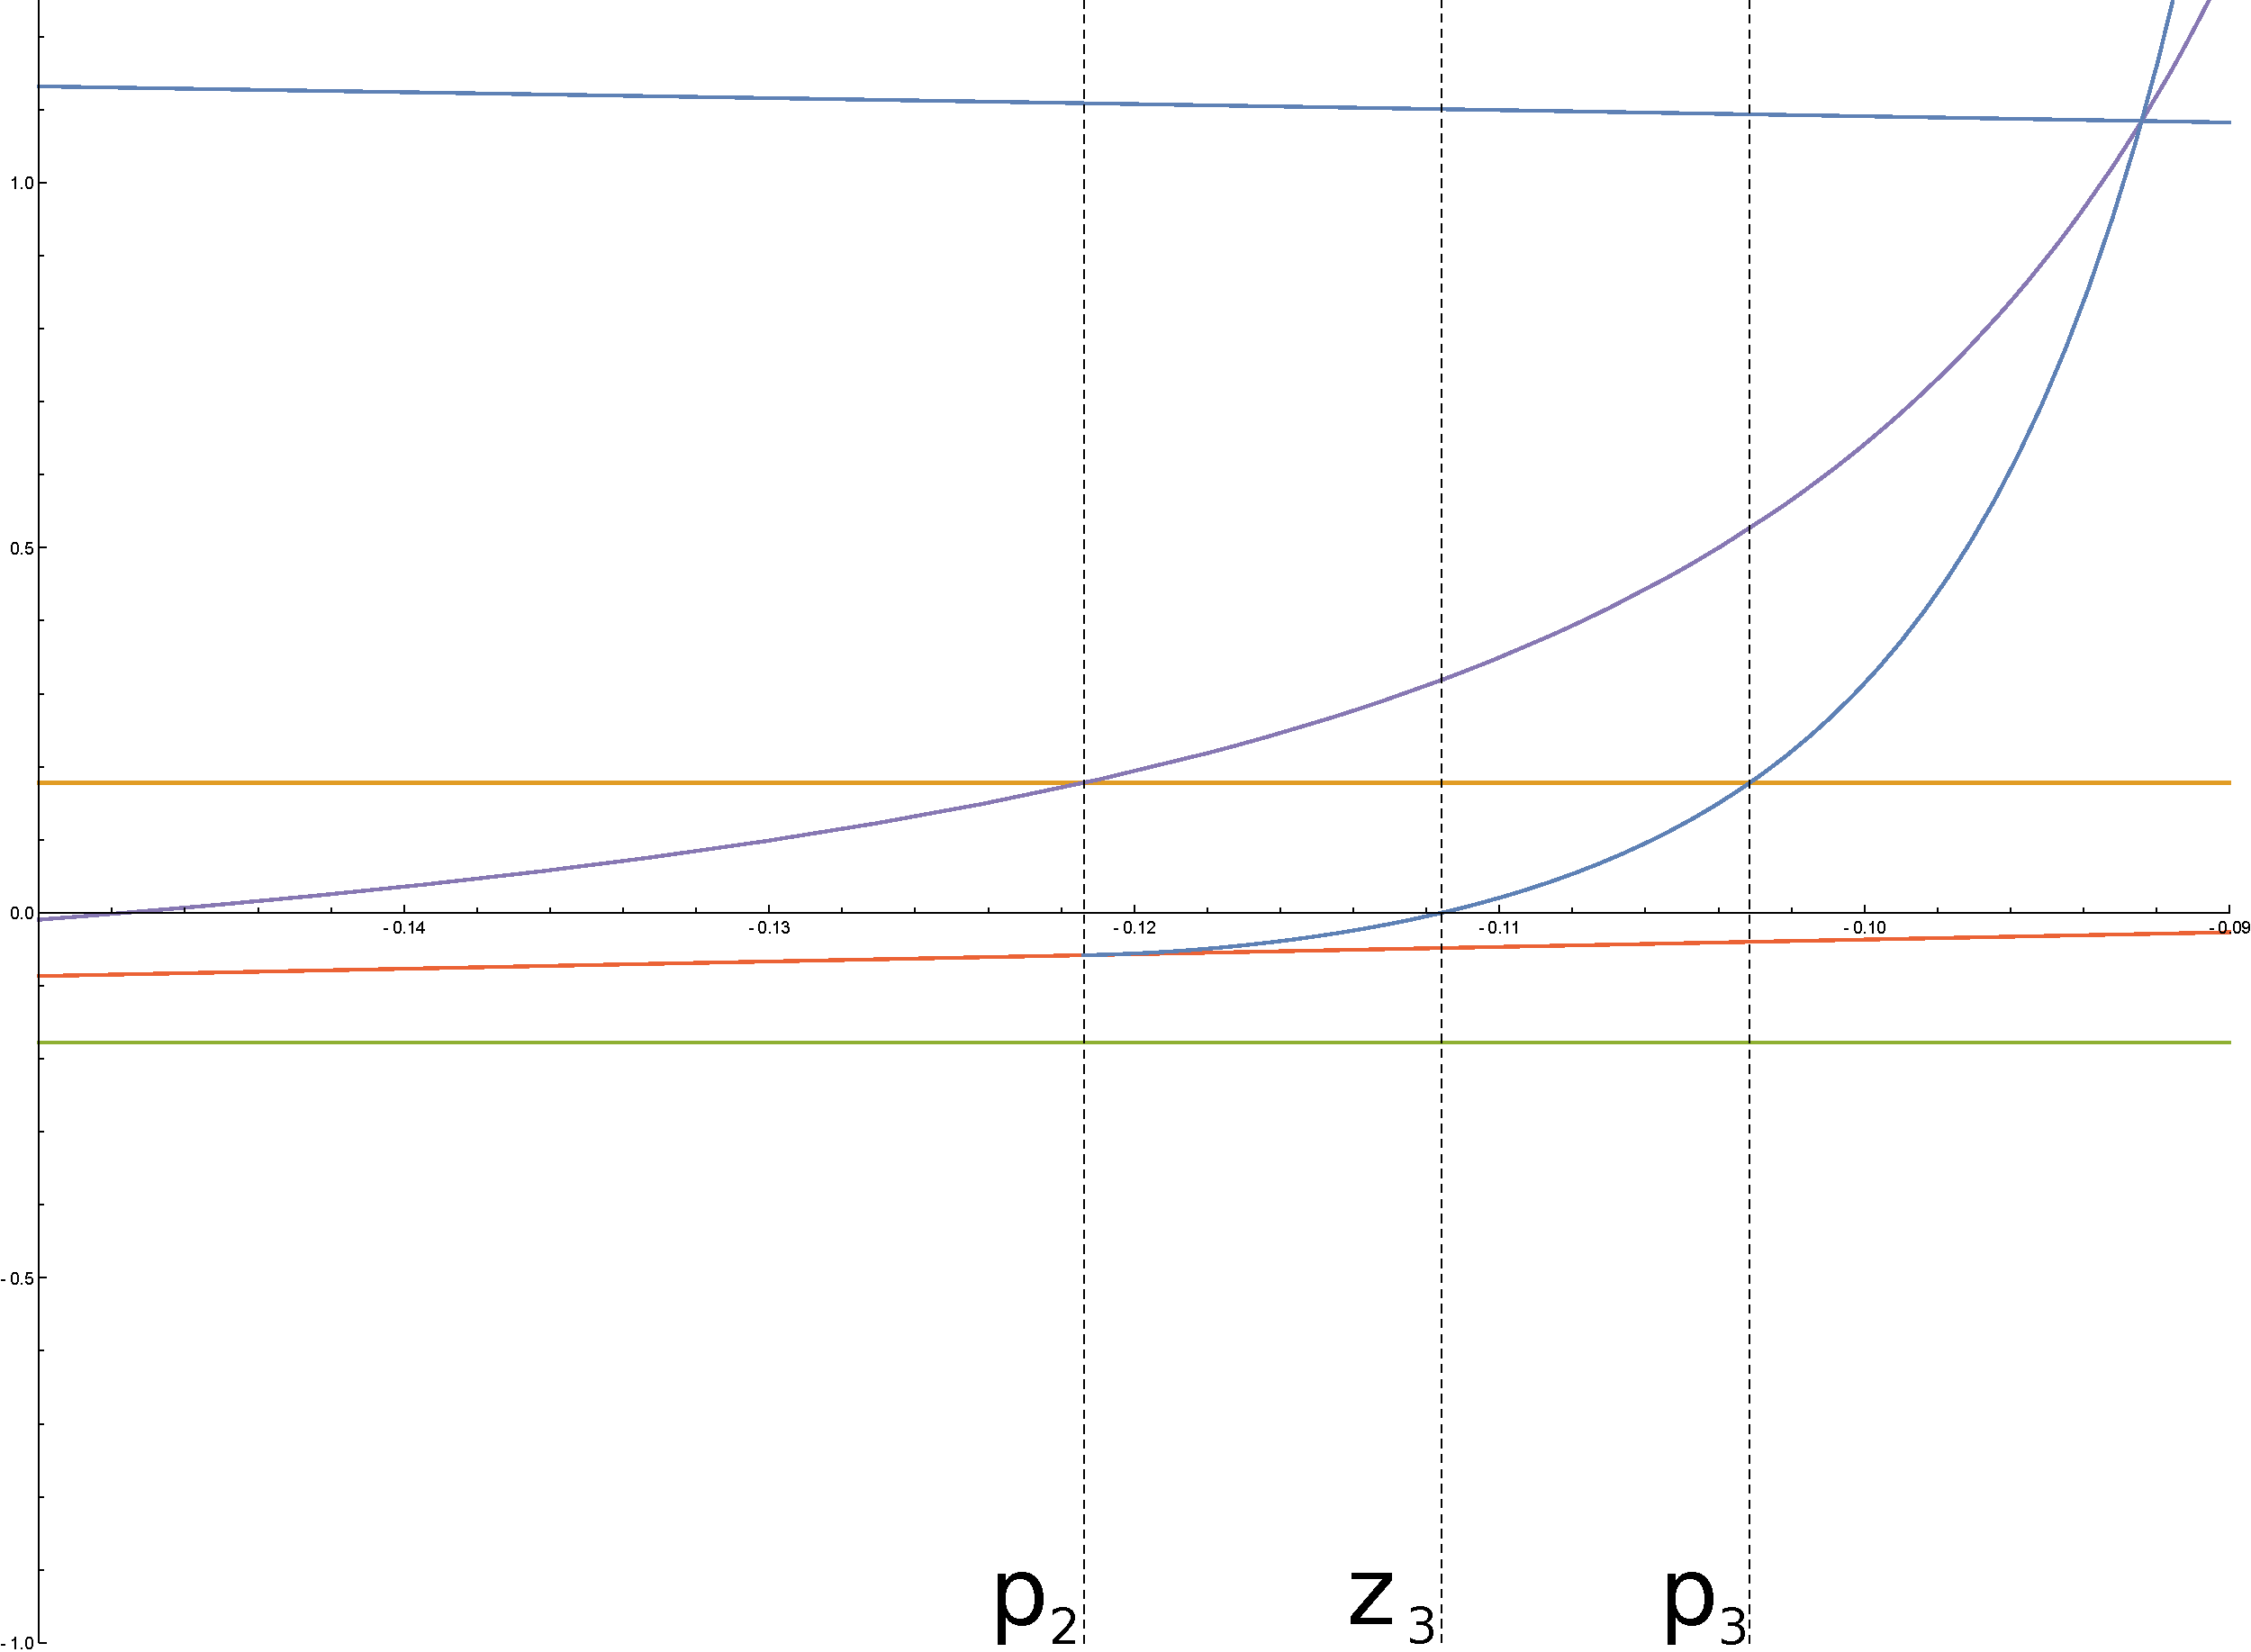
\includegraphics[width=\textwidth]{./img/cplot2H}
				\caption{$n=3$}
				\label{fig:cplot2H}
		\end{subfigure}
		\begin{subfigure}[b]{0.5\textwidth}
				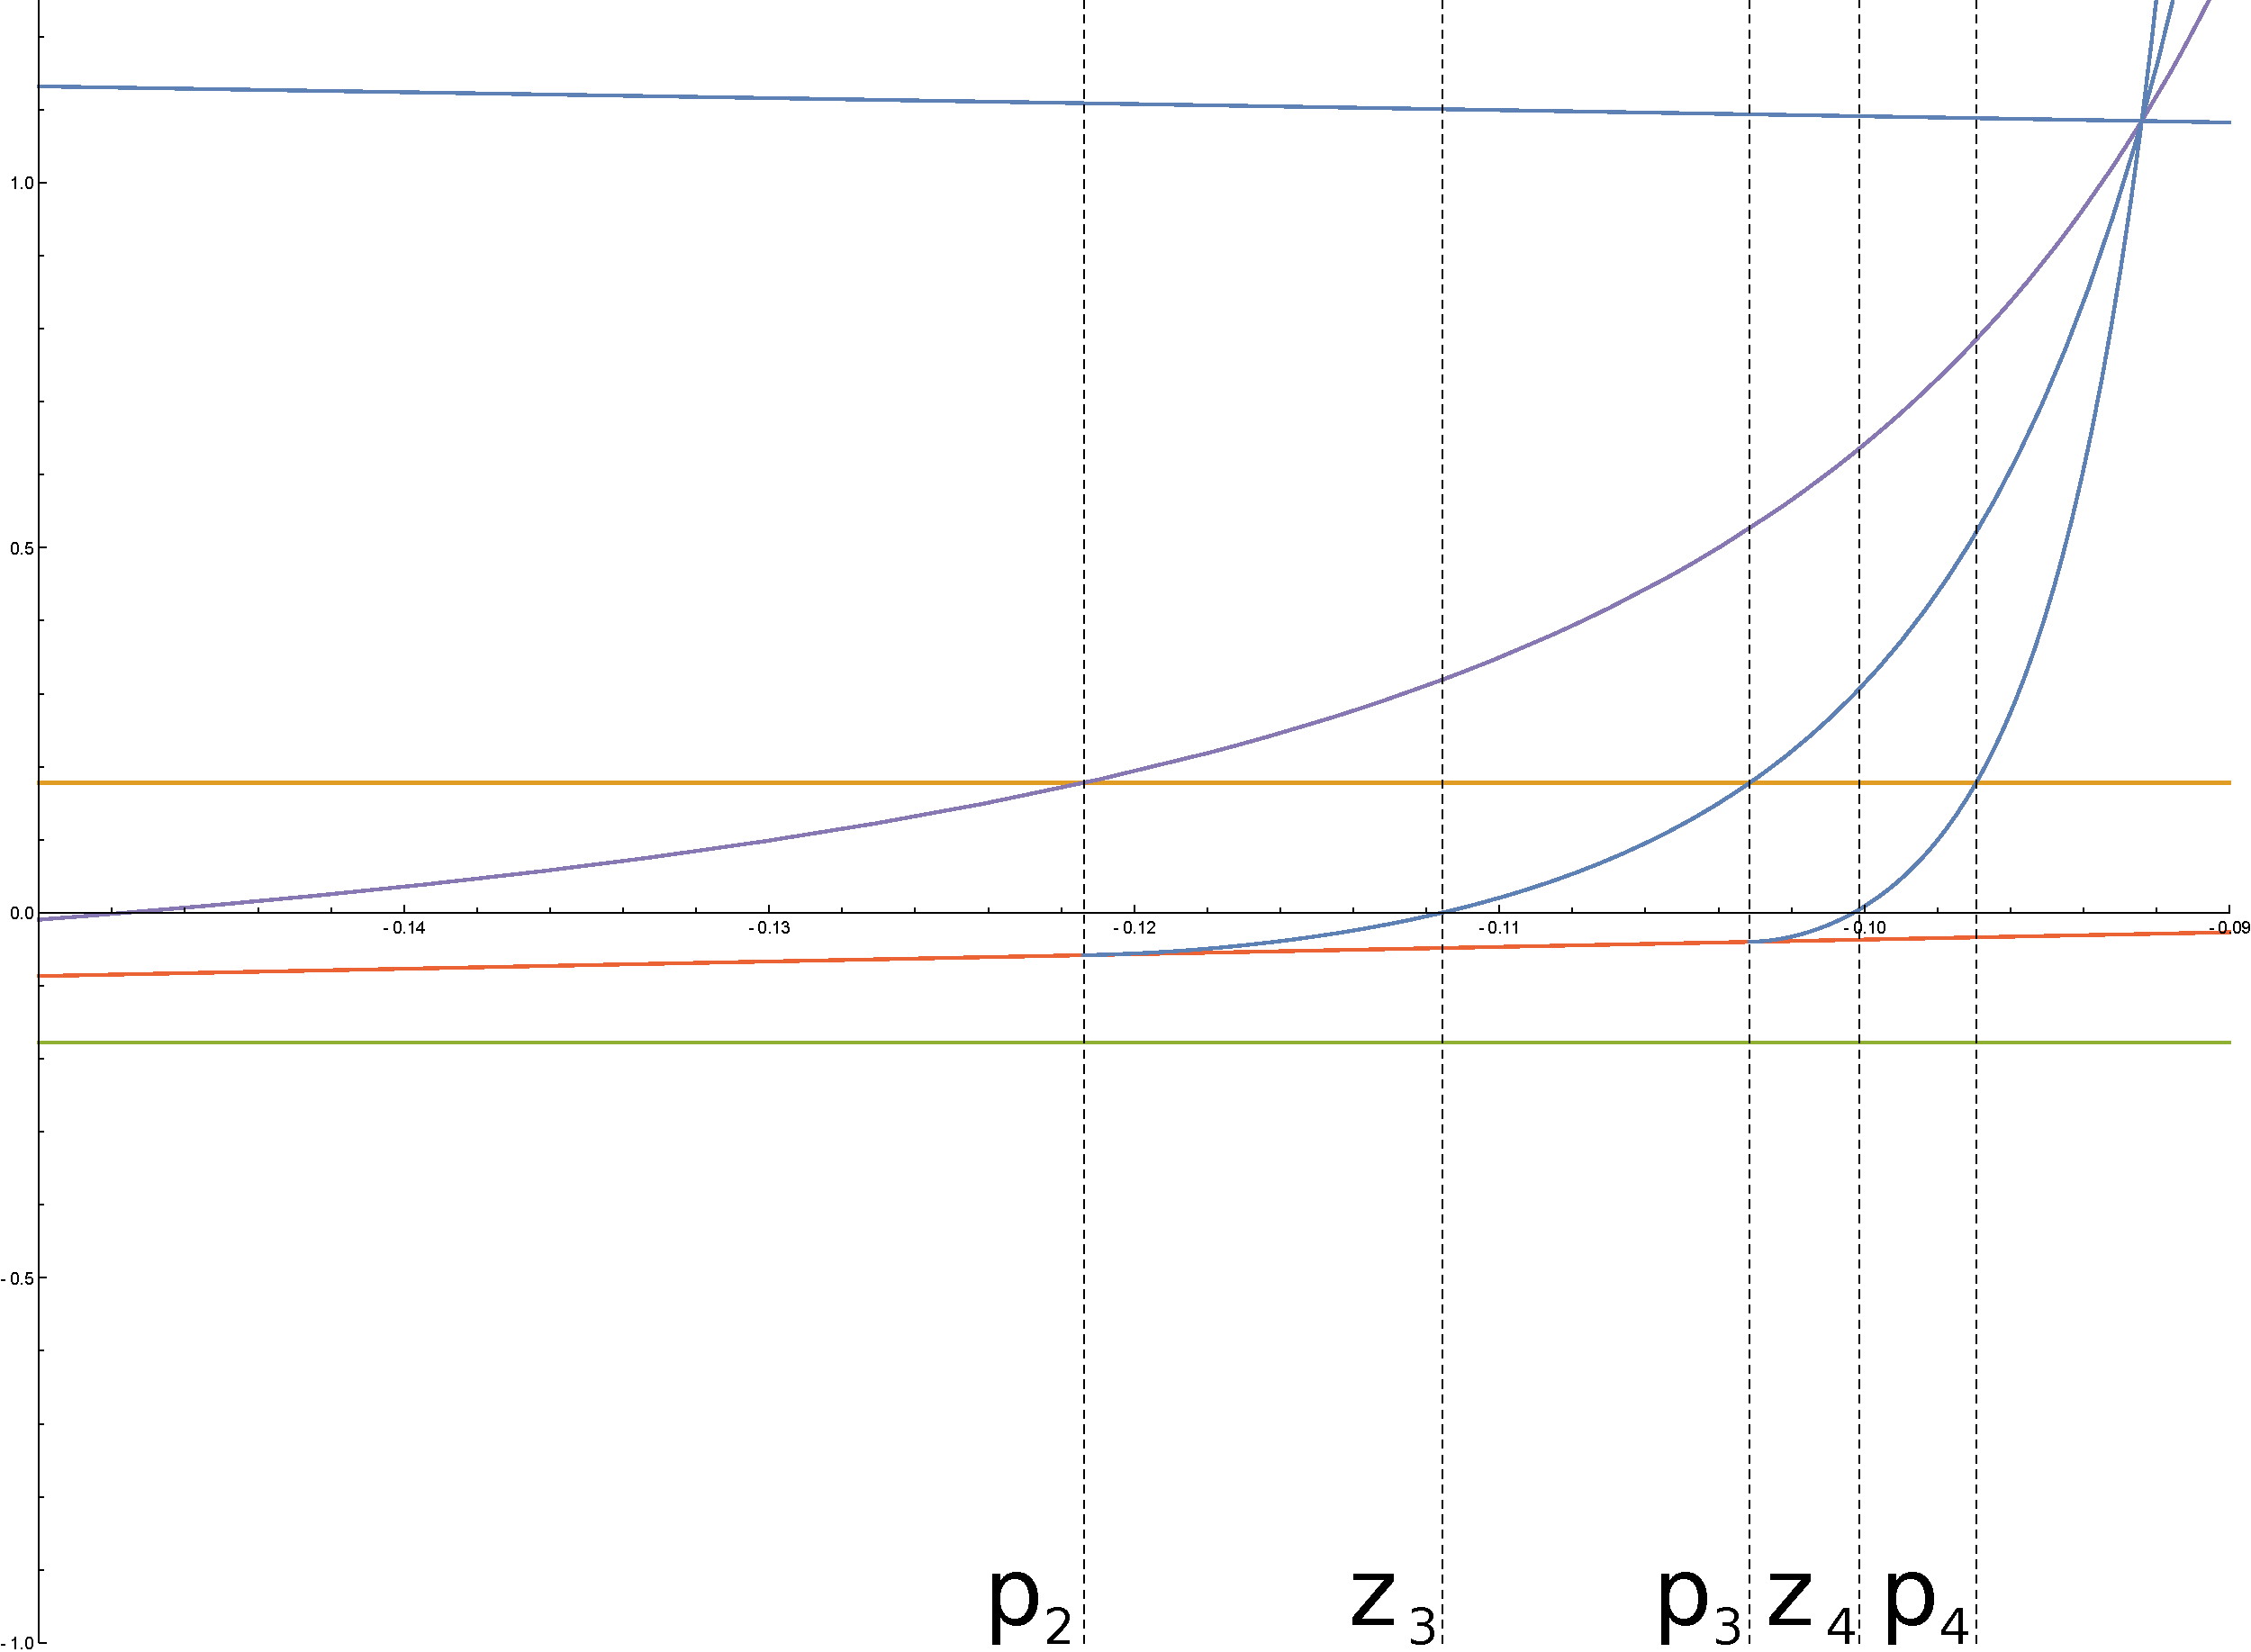
\includegraphics[width=\textwidth]{./img/cplot3H}
				\caption{$n=4$}
				\label{fig:cplot3H}
		\end{subfigure}%
		~ %add desired spacing between images, e. g. ~, \quad, \qquad, \hfill etc.
		  % (or a blank line to force the subfigure onto a new line)
		\begin{subfigure}[b]{0.5\textwidth}
				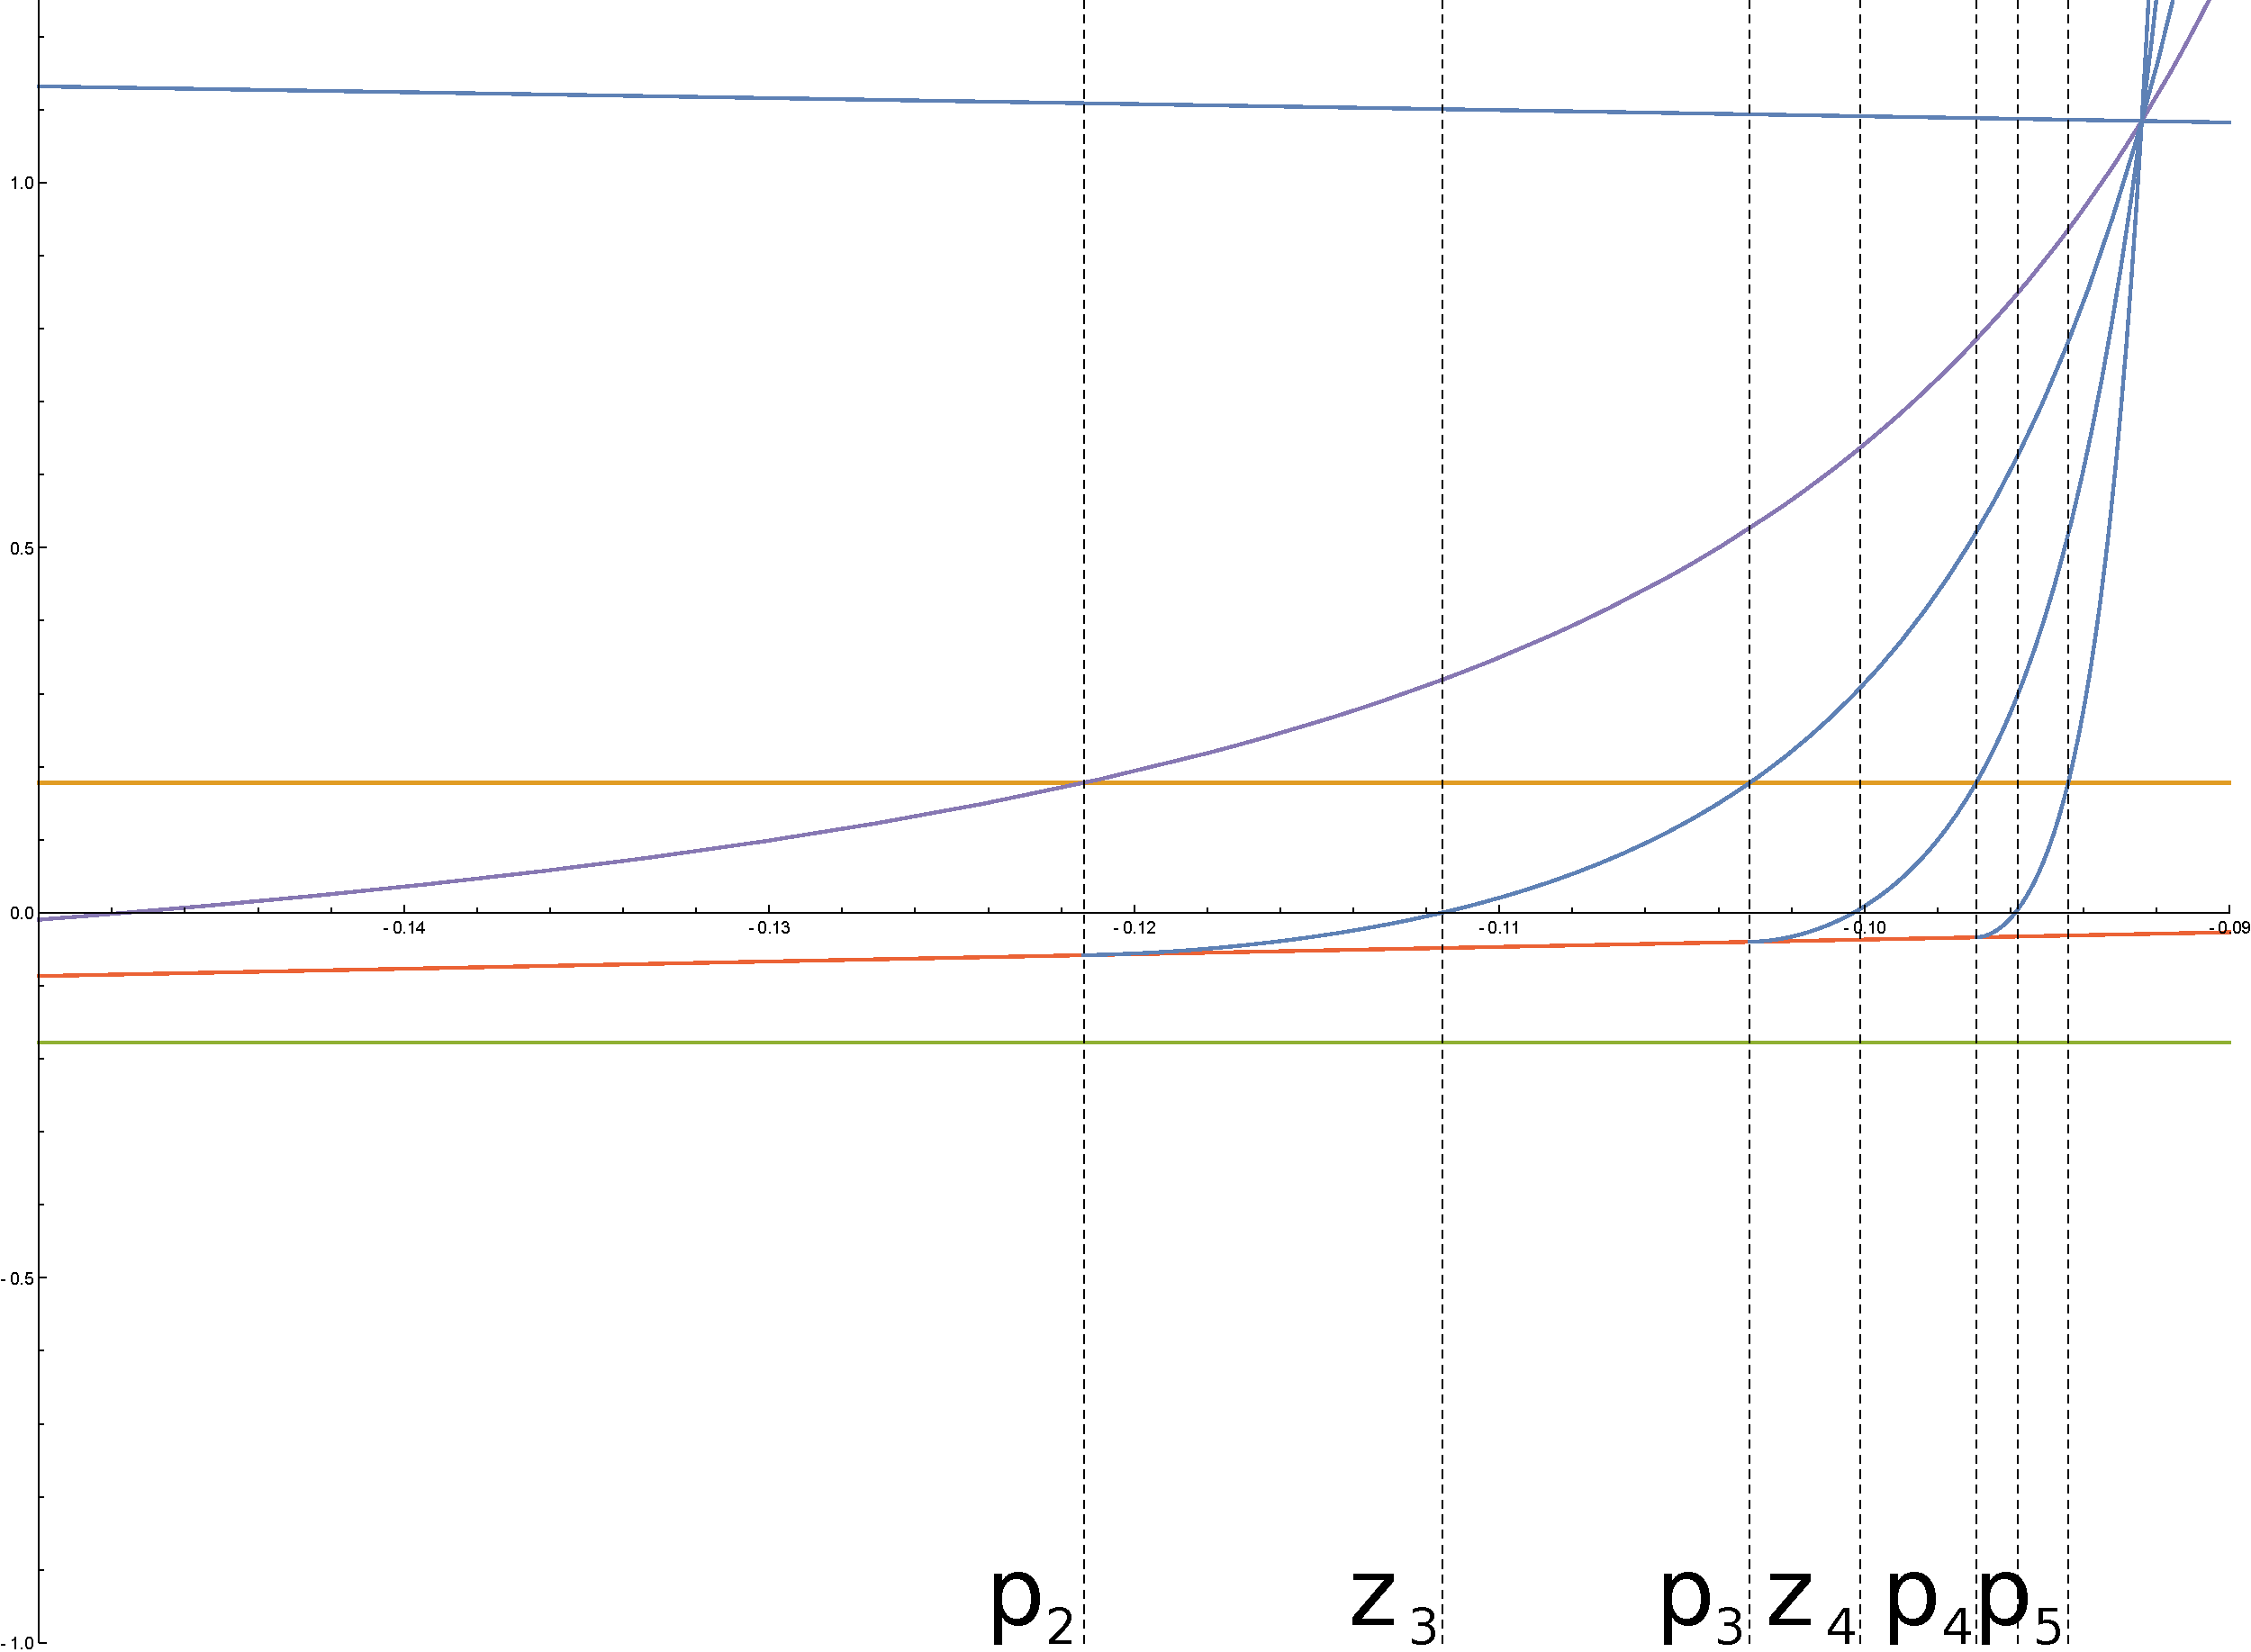
\includegraphics[width=\textwidth]{./img/cplot4H}
				\caption{$n=5$}
				\label{fig:cplot4H}
		\end{subfigure}
		\begin{subfigure}[b]{0.5\textwidth}
				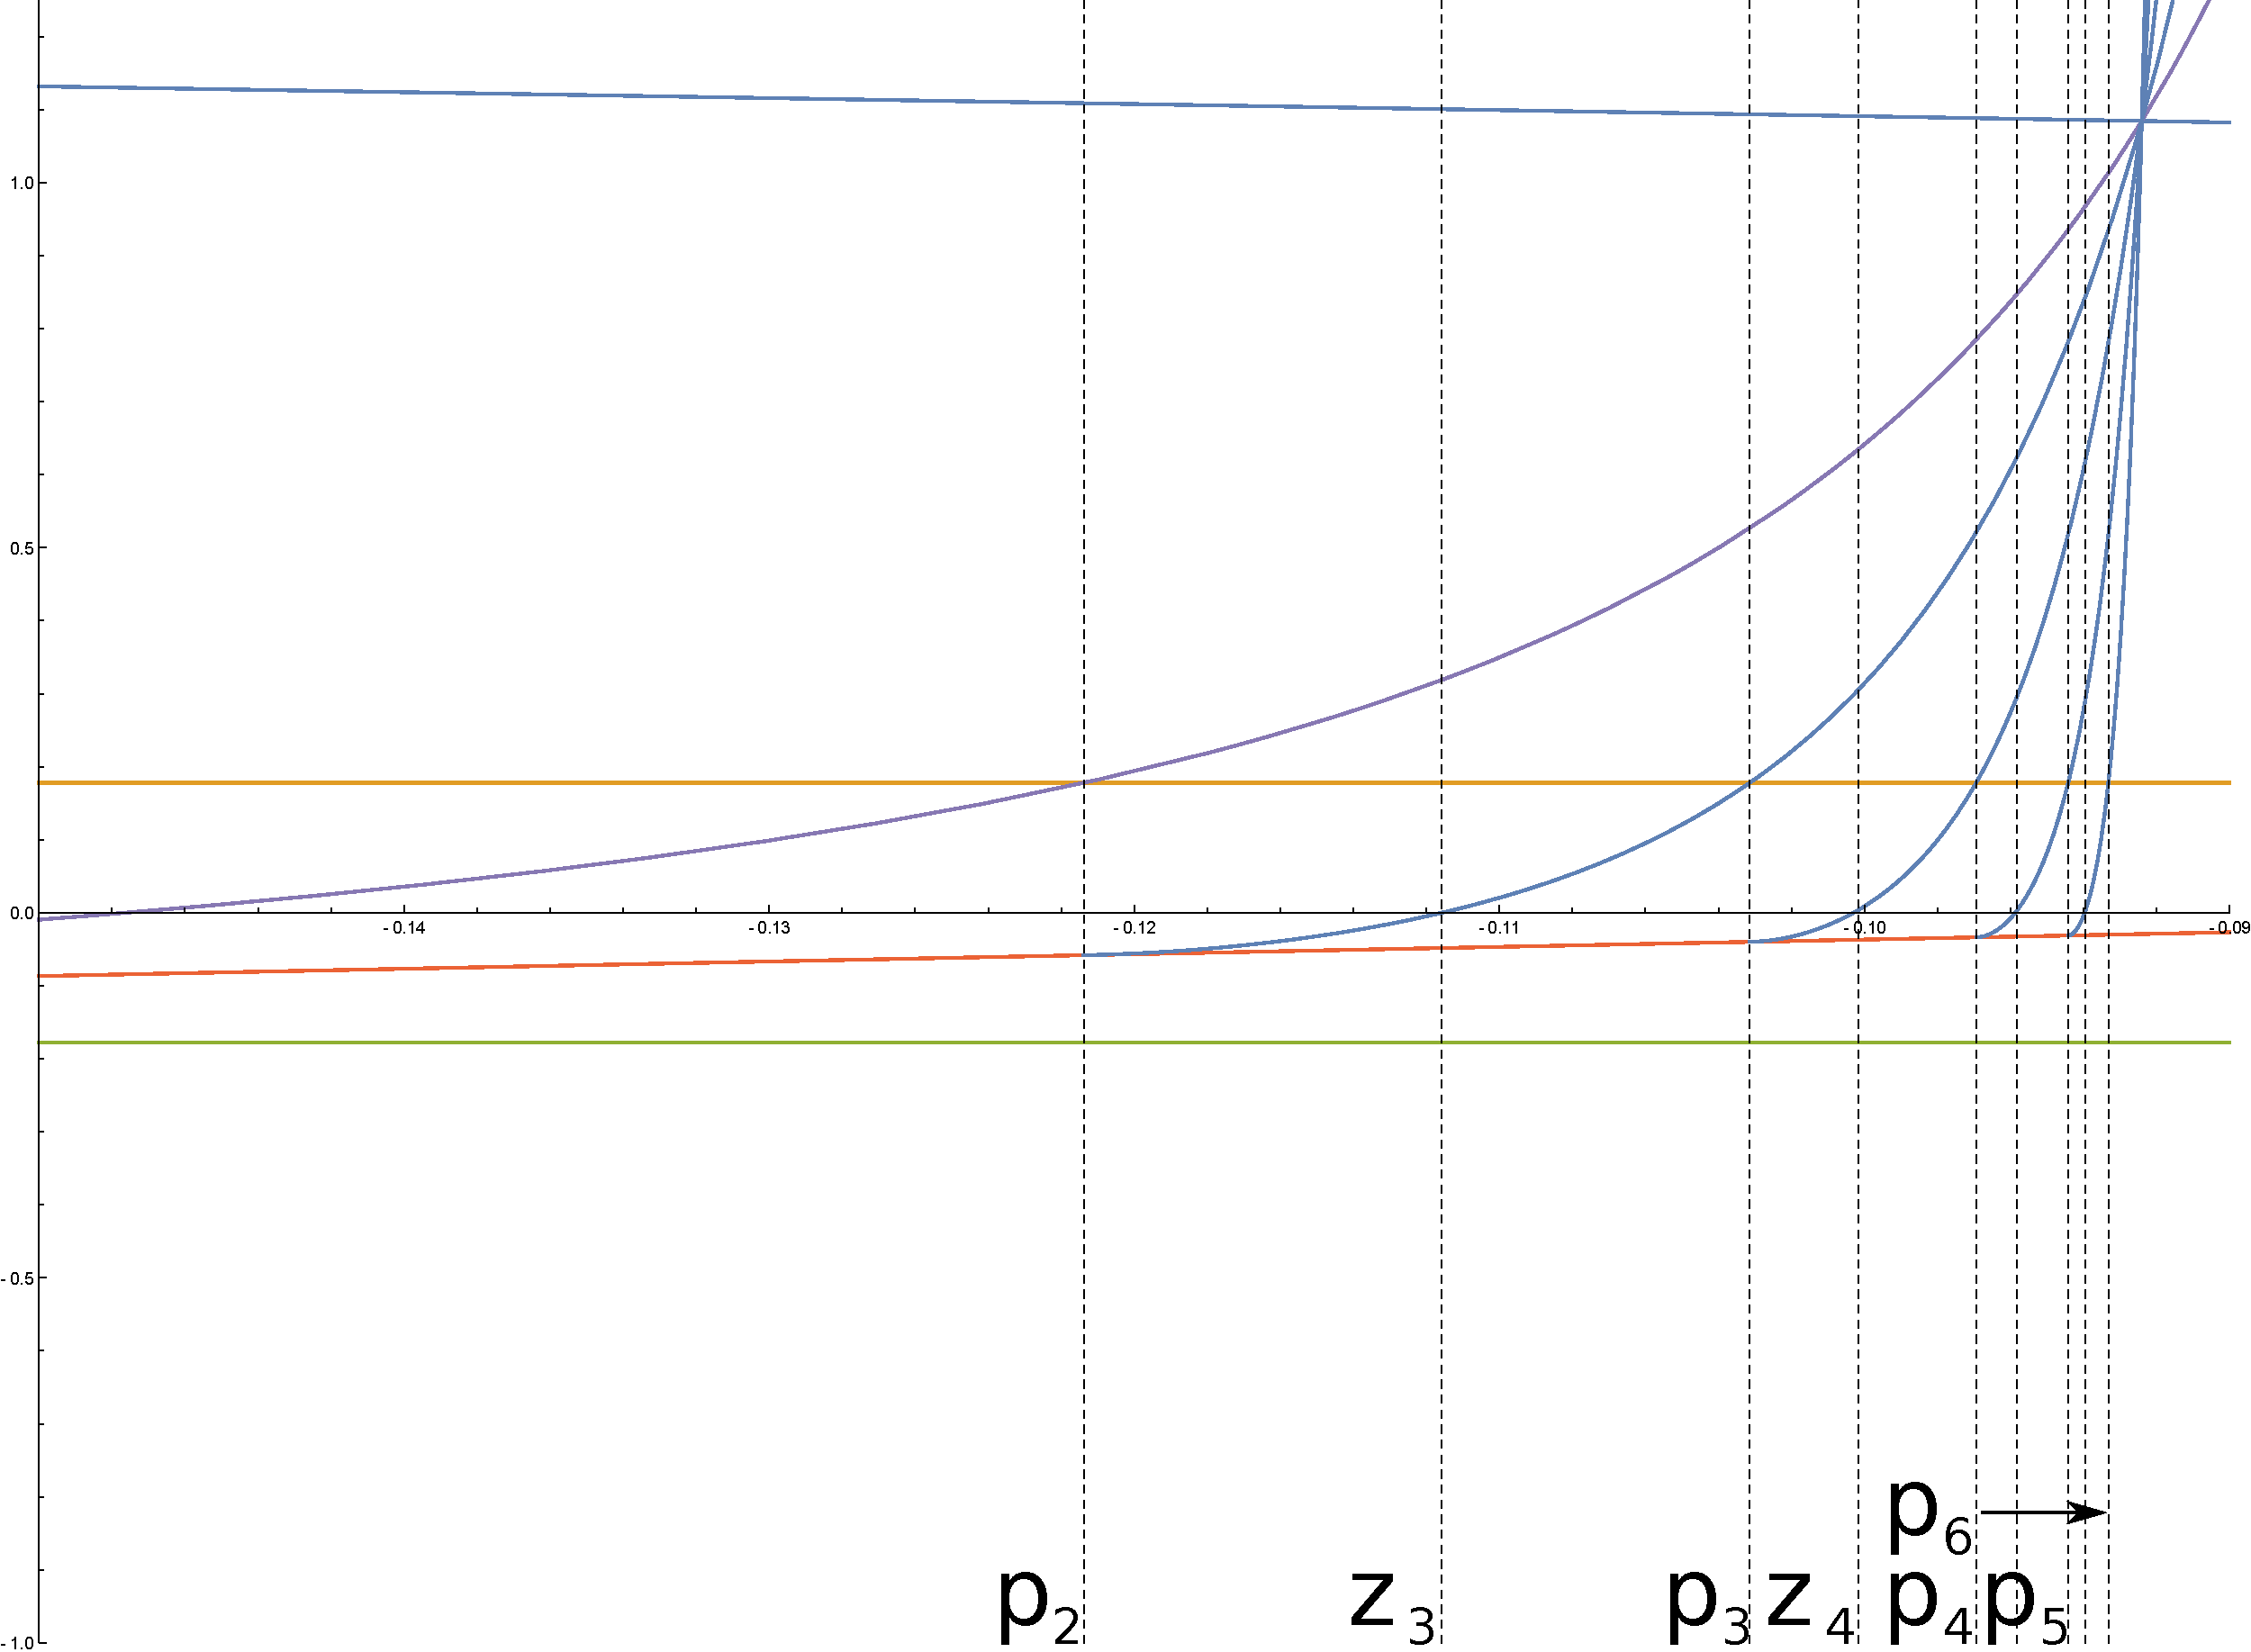
\includegraphics[width=\textwidth]{./img/cplot5H}
				\caption{$n=6$}
				\label{fig:cplot5H}
		\end{subfigure}%
		~ %add desired spacing between images, e. g. ~, \quad, \qquad, \hfill etc.
		  % (or a blank line to force the subfigure onto a new line)
		\begin{subfigure}[b]{0.5\textwidth}
				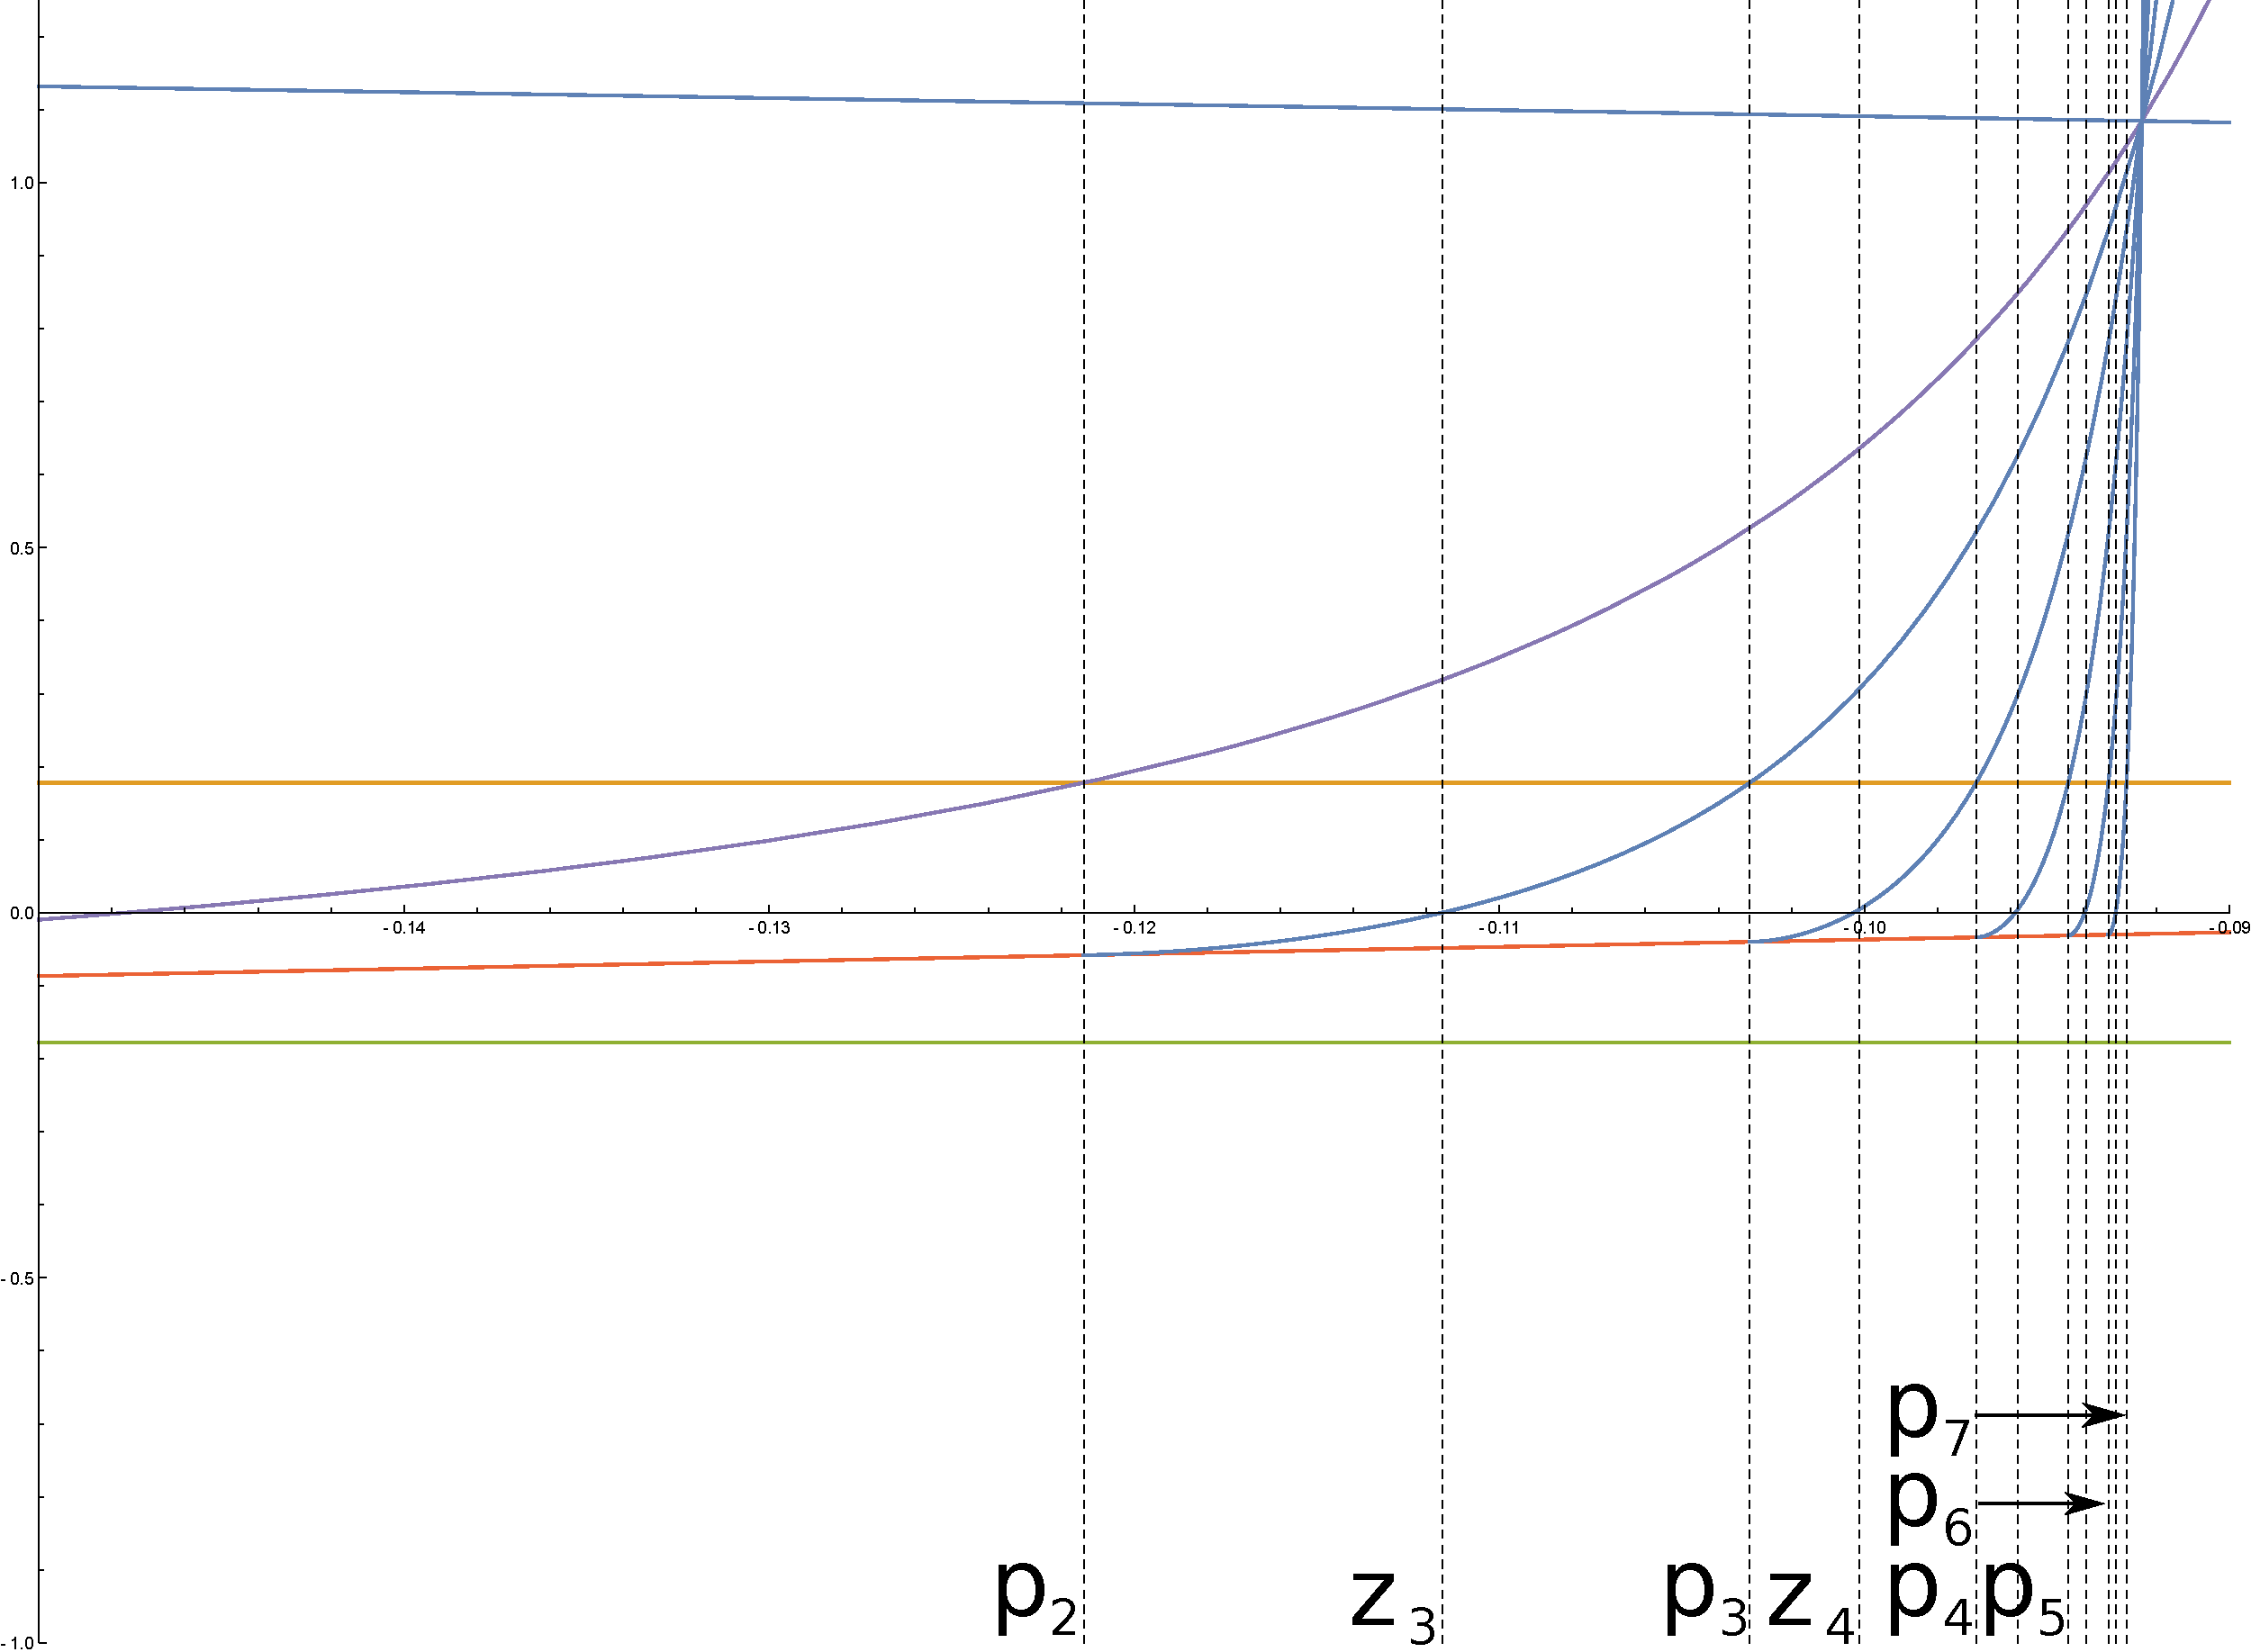
\includegraphics[width=\textwidth]{./img/cplot6H}
				\caption{$n=7$}
				\label{fig:cplot6H}
		\end{subfigure}
		~ %add desired spacing between images, e. g. ~, \quad, \qquad, \hfill etc.
		  % (or a blank line to force the subfigure onto a new line)
		\caption{Plots of various iterates of $f_c (C)$ as a function of $c$ depicting the accumulation of prezero and periodic parameter values as we approach $h_2^{CrP_c}$ from the left. Note that for $n > 4$ the $z_n$ values are marked but not labeled. Also observe that each $f^i_c (C)$ is only plotted on the interval $ (p_{i-1}, h_2^{CrP_c})$ in order to highlight specific behaviors}\label{fig:iterh1}
\end{figure}

% \begin{figure}[ht]
% 		\centering
% 		\begin{subfigure}[b]{0.5\textwidth}
% 				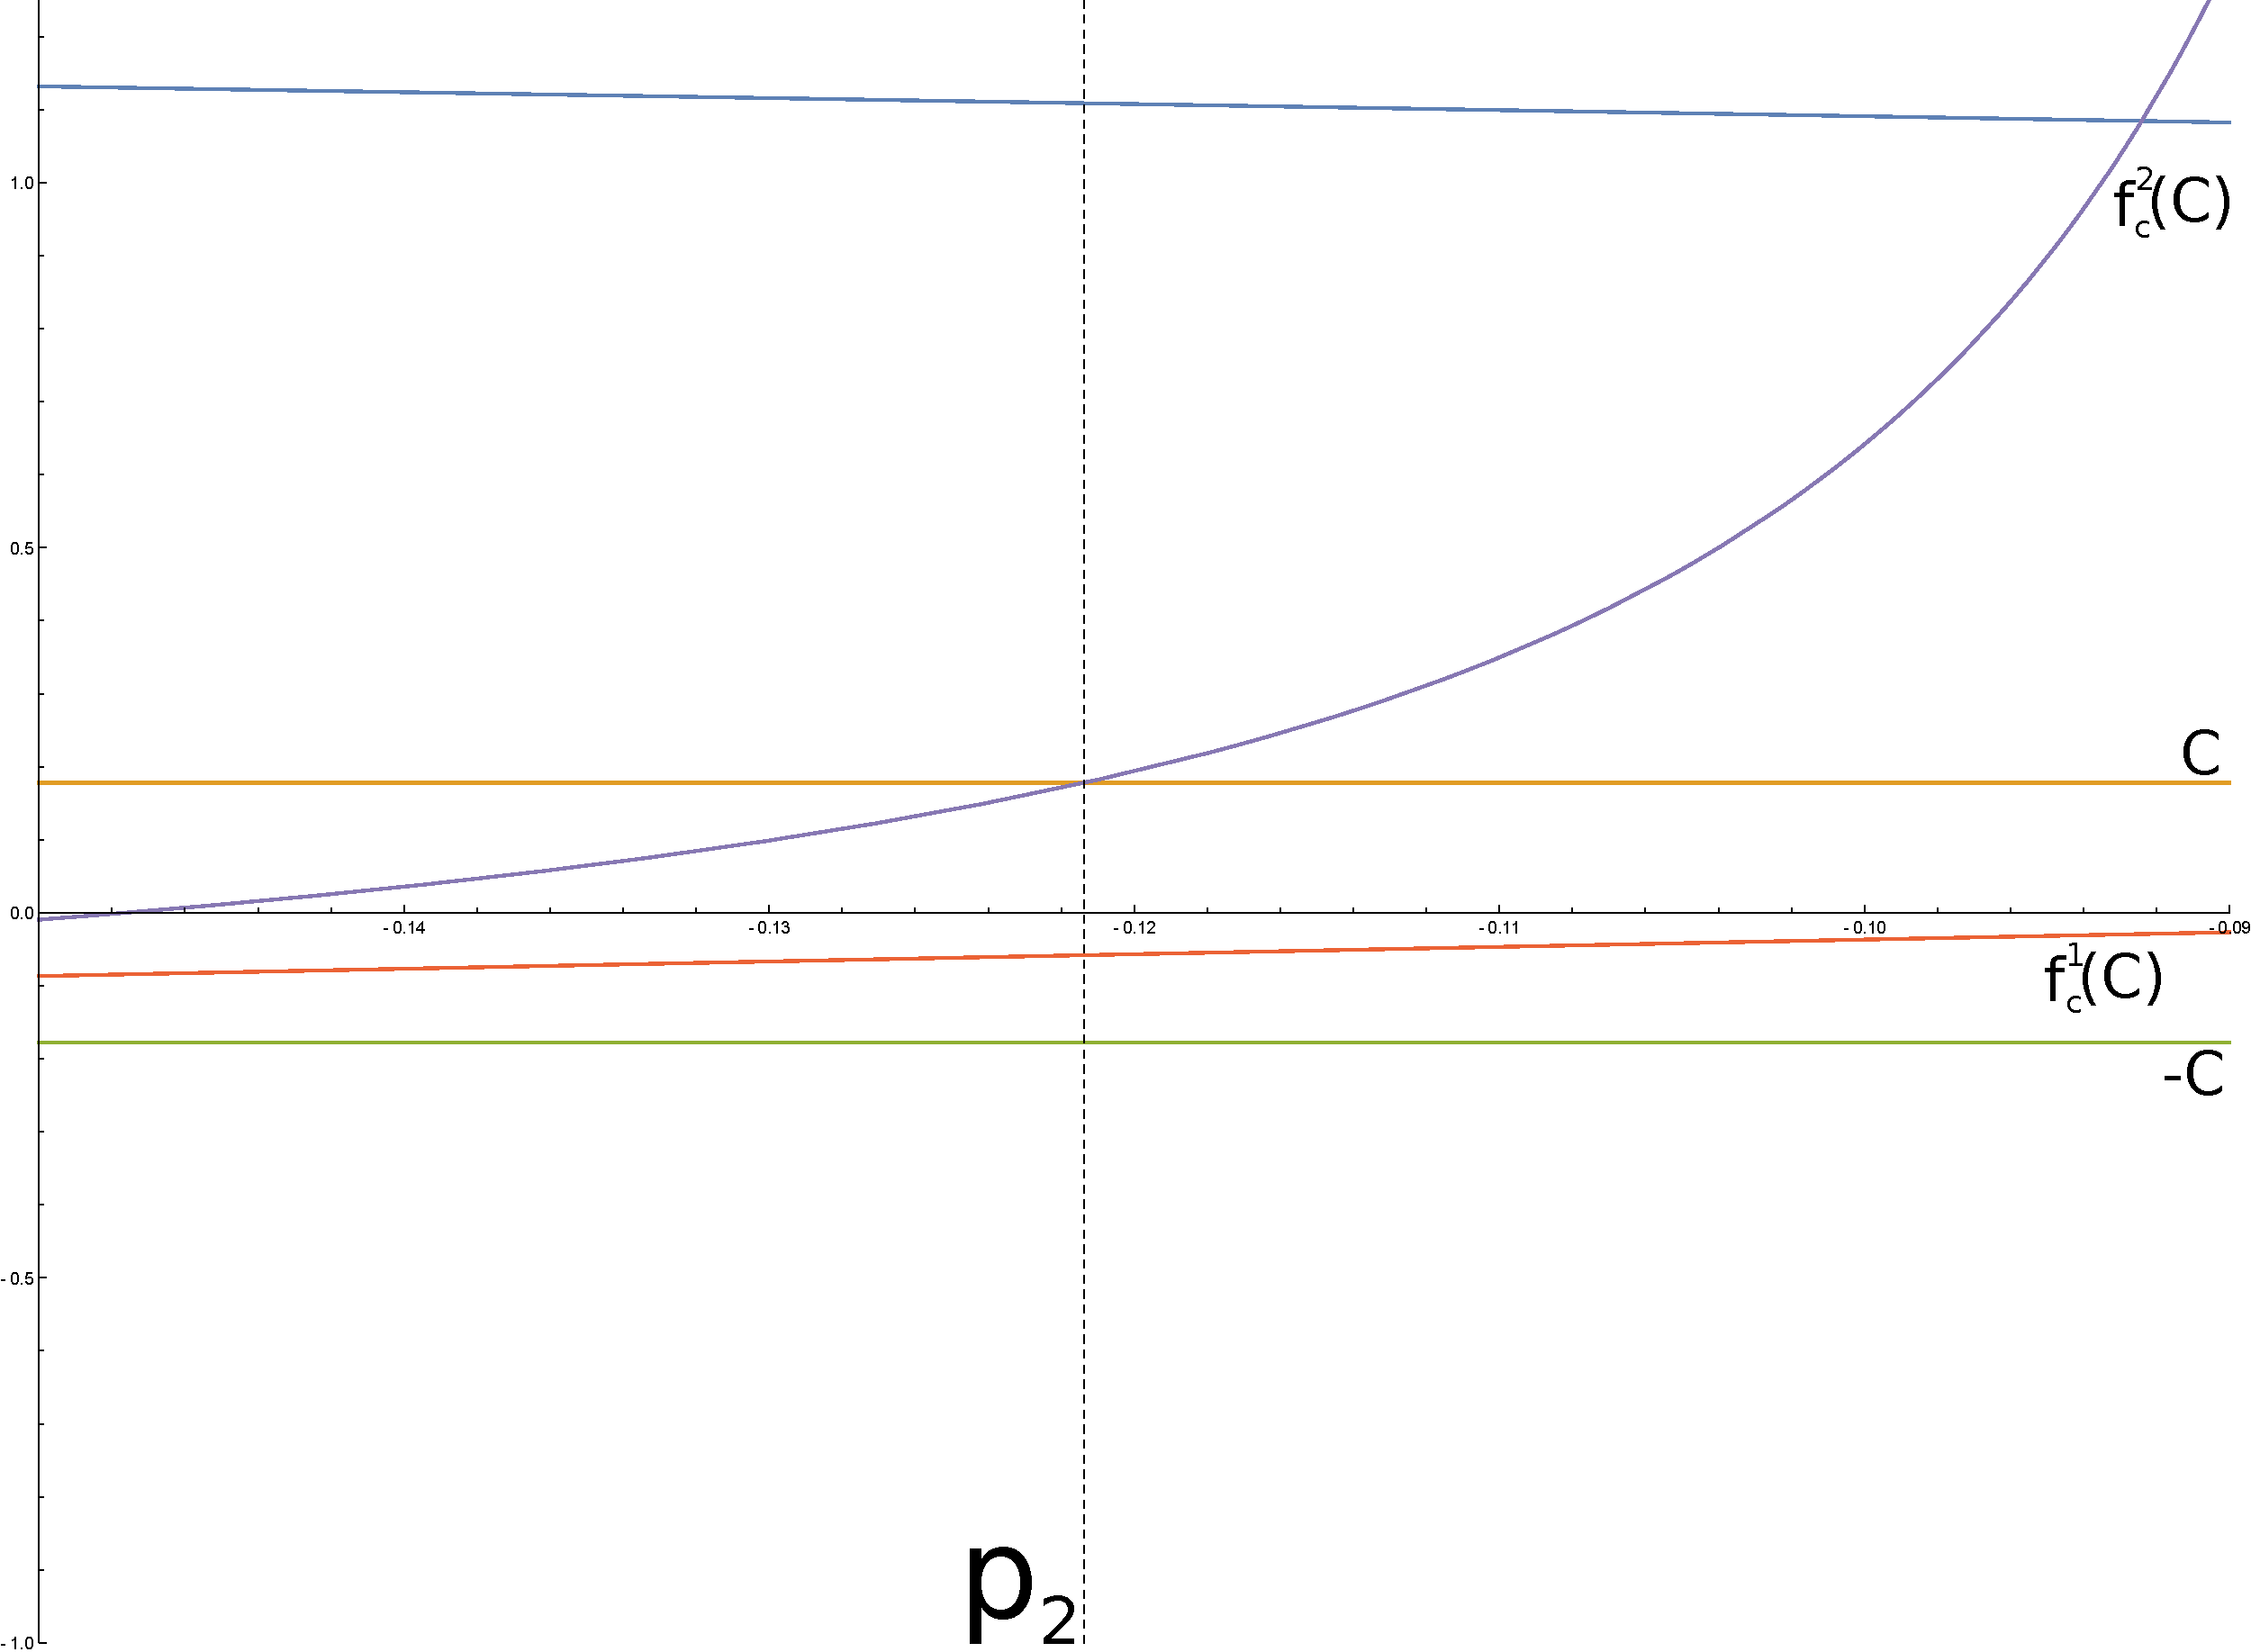
\includegraphics[width=\textwidth]{./img/cplot1H}
% 				\caption{First two iterates of $f_c (C)$ along with the parameter value of its superattracting periodic orbit}
% 				\label{fig:cplot1H}
% 		\end{subfigure}%
% 		~ %add desired spacing between images, e. g. ~, \quad, \qquad, \hfill etc.
% 		  % (or a blank line to force the subfigure onto a new line)
% 		\begin{subfigure}[b]{0.5\textwidth}
% 				\includegraphics[width=\textwidth]{./img/cplot2H}
% 				\caption{Third iterate of $f_c (C)$ added along with the parameter value of its superattracting periodic orbit}
% 				\label{fig:cplot2H}
% 		\end{subfigure}
% 		\begin{subfigure}[b]{0.5\textwidth}
% 				\includegraphics[width=\textwidth]{./img/cplot3H}
% 				\caption{Fourth iterate of $f_c (C)$ added along with the parameter value of its superattracting periodic orbit}
% 				\label{fig:cplot3H}
% 		\end{subfigure}%
% 		~ %add desired spacing between images, e. g. ~, \quad, \qquad, \hfill etc.
% 		  % (or a blank line to force the subfigure onto a new line)
% 		\begin{subfigure}[b]{0.5\textwidth}
% 				\includegraphics[width=\textwidth]{./img/cplot4H}
% 				\caption{Fifth iterate of $f_c (C)$ added along with the parameter value of its superattracting periodic orbit}
% 				\label{fig:cplot4H}
% 		\end{subfigure}
% 		\begin{subfigure}[b]{0.5\textwidth}
% 				\includegraphics[width=\textwidth]{./img/cplot5H}
% 				\caption{Sixth iterate of $f_c (C)$ added along with the parameter value of its superattracting periodic orbit}
% 				\label{fig:cplot5H}
% 		\end{subfigure}%
% 		~ %add desired spacing between images, e. g. ~, \quad, \qquad, \hfill etc.
% 		  % (or a blank line to force the subfigure onto a new line)
% 		\begin{subfigure}[b]{0.5\textwidth}
% 				\includegraphics[width=\textwidth]{./img/cplot6H}
% 				\caption{Seventh iterate of $f_c (C)$ added along with the parameter value of its superattracting periodic orbit}
% 				\label{fig:cplot6H}
% 		\end{subfigure}
% 		~ %add desired spacing between images, e. g. ~, \quad, \qquad, \hfill etc.
% 		  % (or a blank line to force the subfigure onto a new line)
% 		\caption{Plots depicting the accumulation of higher order superattracting periodic orbits near $\pr$}\label{fig:iterh}
% \end{figure}

\begin{figure}[ht]
		\centering
		\begin{subfigure}[b]{0.5\textwidth}
				\includegraphics[width=\textwidth]{./img/cplot1S}
				\caption{First two iterates of $f_c (C)$ along with the parameter value of $f^2_c (C)$'s prezero orbit}
				\label{fig:cplot1S}
		\end{subfigure}%
		~ %add desired spacing between images, e. g. ~, \quad, \qquad, \hfill etc.
		  % (or a blank line to force the subfigure onto a new line)
		\begin{subfigure}[b]{0.5\textwidth}
				\includegraphics[width=\textwidth]{./img/cplot2S}
				\caption{Third iterate of $f_c (C)$ added along with the parameter value of its prezero orbit}
				\label{fig:cplot2S}
		\end{subfigure}
		\begin{subfigure}[b]{0.5\textwidth}
				\includegraphics[width=\textwidth]{./img/cplot3S}
				\caption{Fourth iterate of $f_c (C)$ added along with the parameter value of its prezero orbit}
				\label{fig:cplot3S}
		\end{subfigure}%
		~ %add desired spacing between images, e. g. ~, \quad, \qquad, \hfill etc.
		  % (or a blank line to force the subfigure onto a new line)
		\begin{subfigure}[b]{0.5\textwidth}
				\includegraphics[width=\textwidth]{./img/cplot4S}
				\caption{Fifth iterate of $f_c (C)$ added along with the parameter value of its prezero orbit}
				\label{fig:cplot4S}
		\end{subfigure}
		\begin{subfigure}[b]{0.5\textwidth}
				\includegraphics[width=\textwidth]{./img/cplot5S}
				\caption{Sixth iterate of $f_c (C)$ added along with the parameter value of its prezero orbit}
				\label{fig:cplot5S}
		\end{subfigure}%
		~ %add desired spacing between images, e. g. ~, \quad, \qquad, \hfill etc.
		  % (or a blank line to force the subfigure onto a new line)
		\begin{subfigure}[b]{0.5\textwidth}
				\includegraphics[width=\textwidth]{./img/cplot6S}
				\caption{Seventh iterate of $f_c (C)$ added along with the parameter value of its prezero orbit}
				\label{fig:cplot6S}
		\end{subfigure}
		~ %add desired spacing between images, e. g. ~, \quad, \qquad, \hfill etc.
		  % (or a blank line to force the subfigure onto a new line)
		\caption{Plots of various iterates of $f_c (C)$ as a function of $c$ depicting the accumulation of prezero, periodic, and prefixed parameter values as we approach $s_1^l$ from the right. Note that for $n > 4$ the $z_n$ and $h_n$ values are marked but not labeled. Also observe that each $f^i_c (C)$ is only plotted on the interval $ (p_{1}^{-C}, z_{i-1})$ in order to highlight specific behaviors}\label{fig:iterh2}
\end{figure}
\FloatBarrier

	\section{An Infinite Hierarchy of Prezero Points}

Now that we have visually demonstrated the existence of these two ``primary sequences'' of parameter values, we will introduce some results which add an infinite hierarchy of complexity in between each parameter value in the aforementioned sequences. This result is best summarized by Proposition \ref{mainprop}:

\begin{customthm}{\ref{mainprop}}
	Suppose we have two distinct parameter values $z_{n_1}^{C\alpha0}, z_{n_2}^{C\beta0} \in (\pl, \pr)$ where $\alpha$ and $\beta$ are coding sequences such that $\alpha_i \neq \beta_i$ for at least one $i$. Then there must be at least one other prezero parameter value $z_{n_3}^{C\gamma0}$ on the interval $\inte{z_{n_1}^{C\alpha0}}{z_{n_2}^{C\beta0}}$ such that $\alpha_i \neq \gamma_i$ and $\beta_j \neq \gamma_j$ for at least one $i$ and one $j$.
\end{customthm}

% \begin{figure}[h]
% \centering
% 	\includegraphics[width=.75\textwidth]{./img/cplot.pdf}
% 	\caption{Plot of the first five iterates of $C$ with respect to $c$}
% 	\label{cplot}
% \end{figure}

In this section we will briefly provide some discussion and figures which provide some intuition as to what this proposition means. First consider the plot of the first 3 iterates of the right hand critical point with respect to $c$ as shown in the Figure \ref{hqcplot}. This plot is a useful visual guide because we can quickly see how the behavior of lower iterates affects the behavior of higher iterates. One of the most notable behaviors that can be observed is how some $n^{th}$ iterate mapping to zero forces all higher iterates to be $\infty$, a fact easily proven as Lemma \ref{zero}. Additionally, we note that for all $n > 2$, $f^n_{\pr} (C) = P_c$ and $f^n_{\pl} (C) = -C$ as discussed in the introductory remarks. Thus at either end of this interval, all iterates are clamped to some specific value, regardless of the behavior in between.

To provide an example of what Proposition \ref{mainprop} is saying, we will provide a sample case from the proof of Proposition 4.2. Figure \ref{fig:case1} shows the first case where we have some parameter $z_3^{CrF0}$ to the left and some parameter $z_4^{CrFL0}$ to the right. This proposition forces the existence of some other $z_{n_1}$ between these two parameter values. Two satisfactory parameter values are labeled as $z_5^{CrFLF0}$ and $z_5^{CrFLL0}$. Note that these values were found by looking at $f^4_c (C)$ which has a parameter value $p_4^{CrFL}$ in between $z_3^{CrF0}$ and $z_4^{CrFL0}$. Then we show in Chapter 4 that $f^1_c (C) < 0$ for $c \in (\pl, \pr)$, meaning that when we look at the fifth iterate at this parameter value we get:
\[
	f^5_{p_4^{CrFLC}} (C) = f_{p_4^{CrFLC}}\left (f^4_{p_4^{CrFLC}} (C)\right) = f_{p_4^{CrFLC}} (C) < 0
\]
Thus we have a $c$ value for which $f^5_c (C) < 0$ and two points where the fifth iterate must be $\infty$ (at $z_3^{CrF0}$ and $z_4^{CrFL0}$) so in between there must be two points where the fifth iterate is 0, these being $z_5^{CrFLF0}$ and $z_5^{CrFLL0}$. 
\begin{figure}
	\centering
	\includegraphics[width=.75\textwidth]{./img/pre0case1p}
	\caption{Plot of $f_c (C),f^3_c (C),f^4_c (C)$ and part of $f^5_c (C)$ showing the existance of two prezero parameter values $z_5^{CrFLF0}$ and $z_5^{CrFLL0}$ between the outer two prezero parameter values $z_3^{CrF0}$ and $z_4^{CrFL0}$}
	\label{fig:case1}
\end{figure}

In Chapter 4 we prove this for all $n$. An interesting implication of this theorem is that there are in fact an infinity of $z_n$ values between any other $z_{n_1}, z_{n_2} \in (\pl, \pr)$ which additionally gives an infinity of $h_n$ and $p_n$ values as well. Thus the primary sequences we discussed in the previous section are just the first level of critical point behavior, giving rise to the infinite hierarchy that Proposition \ref{mainprop} fills in.





%Another note about Figure \ref{cplot} is that each curve varies continuous with respect to $c$ and $x$, as shown in Proposition \ref{contin}. This fact opens the door to many Intermediate Value Theorem arguments that we see in the next chapter. 
